\documentclass[twoside,12pt]{book}

\usepackage[utf8]{inputenc}
\usepackage[english]{babel}
\usepackage{geometry}
\usepackage{graphicx}
\usepackage{epsfig}
\usepackage[labelfont=bf,skip=0px]{caption}
\usepackage{subfloat}
\usepackage[labelfont=bf,justification=centering,skip=0px]{subcaption}
\usepackage{booktabs}
\usepackage{float}
\usepackage{makeidx}
% \usepackage[nottoc,notlot,notlof]{tocbibind}
\usepackage{supertabular}
\usepackage{array}
\usepackage{setspace}
\usepackage{layout}
\usepackage{enumerate}
\usepackage{rotating}
\usepackage{bbm}
\usepackage{moreverb}
\usepackage{tikz}
\usepackage{multirow,tabularx,bigdelim}
\usepackage{makecell}
\usepackage{amsmath}
\usepackage{amsthm}
\usepackage{amssymb}
\usepackage{mathtools}
% \usepackage{captcont}
\usepackage{verbatim}
\usepackage{titlesec}
\usepackage{url,paralist}
\usepackage{subfiles}
\usepackage{listings}
\usepackage[inline]{enumitem}
\usepackage{stmaryrd}
\usepackage{lipsum}
\usepackage{lscape}
\usepackage{color}
\usepackage{xr}
\usepackage{float}
\usepackage{longtable}
\usepackage{etoolbox}
\usepackage{wrapfig}
\usepackage{relsize}
\usepackage[noline,ruled]{algorithm2e}
\usepackage{fontspec}
\usepackage{arydshln}
\usepackage{bm}
\usepackage[toc,page]{appendix}
\usepackage[pdfpagemode={UseOutlines},bookmarks=true,bookmarksopen=true, pdfauthor={Indrajit Banerjee},pdfcreator={Indrajit Banerjee}, bookmarksopenlevel=0,bookmarksnumbered=true,hypertexnames=false, colorlinks,linkcolor={black},citecolor={black},urlcolor={red},  pdfstartview={FitV},unicode,breaklinks=true]{hyperref}
\usepackage{cleveref}

\usetikzlibrary{arrows, quotes,shapes,positioning, calc}

\newtheorem{theorem}{Theorem}

\newenvironment{proofsketch}{\renewcommand{\proofname}{Proof Sketch}\proof}{\endproof}

\lstdefinelanguage{All}[]{C}{
  morekeywords={if,then,else,match,with,let,in,fn,type,i32,i8,bool,false,true,List,lnode,Str,clnode,u32,is,assume,assuming,do,sizeof,offsetof,typeof,addrof}
}

\lstnewenvironment{allLangEnvFoot}{\lstset{language=All,basicstyle=\footnotesize\ttfamily,mathescape=true}}{}
\lstnewenvironment{allLangEnvScript}{\lstset{language=All,basicstyle=\scriptsize\ttfamily,mathescape=true}}{}

\lstset{%
    language     = C,
    keywordstyle = \color{myastral},
    stringstyle  = \color{red},
    breaklines = false,
    commentstyle=\color{mygreen},
    keepspaces=true,
    escapeinside = ~~,
    showlines = true,
%    numbers=left,
%    numberstyle=\tiny\color{mygray},
%    numbersep=2pt,
}

\usepackage{stackengine}
\usepackage{backnaur}
\usepackage{xcolor}
\usepackage{mathtools}
\usepackage{accents}

\newcommand{\xmark}{\ding{55}}%
\newcommand{\rulesep}{\unskip\ \vrule\ }

\setlength{\textfloatsep}{6.0pt plus 1.0pt minus 1.0pt}
\setlength{\intextsep}{3.0pt plus 0.5pt minus 0.5pt}

\makeatletter
\newcommand{\oset}[3][0ex]{%
  \mathrel{\mathop{#3}\limits^{
    \vbox to#1{\kern-2\ex@
    \hbox{$\scriptstyle#2$}\vss}}}}
\makeatother

\newcommand{\toolName}{S2C}%
\newcommand{\ite}[3]{\ensuremath{#1?#2:#3}}%
\newcommand{\sumDtor}{\underline{\tt if}-\underline{\tt then}-\underline{\tt else}}%
\newcommand{\sumIs}[2]{\ensuremath{#1\ \mathrm{is}\ \cons{#2}}}%
\newcommand{\fieldPath}[2][\ensuremath{.}]{%
  \def\nextitem{\def\nextitem{#1}}% Separator
  \renewcommand*{\do}[1]{\nextitem{\field{##1}}}% How to process each item
  \docsvlist{#2}% Process list
}
\newcommand{\prodAccess}[2]{\ensuremath{#1.{\fieldPath{#2}}}}%
\newcommand{\sumIf}[1]{\underline{\tt if}\ \ensuremath{#1}}%
\newcommand{\sumThen}[1]{\underline{\tt then}\ \ensuremath{#1}}%
\newcommand{\sumElif}[1]{\underline{\tt elif}\ \ensuremath{#1}}%
\newcommand{\sumElse}[1]{\underline{\tt else}\ \ensuremath{#1}}%
\newcommand{\recursiveRelations}{recursive relations}%
\newcommand{\recursiveRelation}{recursive relation}%
\newcommand{\SpecL}{Spec}%
\newcommand{\indEq}{\ensuremath{\sim}}%
\newcommand{\indEqDepth}[1]{\ensuremath{\sim_{#1}}}%
\newcommand{\indEqUapprox}[1]{\ensuremath{\approx_{#1}}}%
\newcommand{\depthBound}[2]{\ensuremath{\Gamma_{#1}(#2)}}%
% \newcommand{\structPointer}[4]{\ensuremath{{#1} \oset{#2}{\rightarrow}_{\type{#3}} {\field{#4}}}}%
\newcommand{\structPointer}[4]{\ensuremath{{#1} \overset{#2}{\rightarrow}_{\type{#3}} {\field{#4}}}}%
\newcommand{\arrIndex}[4]{\ensuremath{#1[#2]_{#3}^{\type{#4}}}}%
\newcommand{\memRead}[3]{\ensuremath{#1[#2]_{\type{#3}}}}%
\newcommand{\memWrite}[4]{\ensuremath{#1[#2 \leftarrow #3]_{\type{#4}}}}%
\newcommand{\pointsTo}{\ensuremath{\rightsquigarrow}}%
\newcommand{\hoareTriple}[3]{\ensuremath{\{#1\}(#2)\{#3\}}}%
\newcommand{\lift}[3]{\ensuremath{{{\tt C#1}_{#2}^{\tt #3}}}}%
\newcommand{\lifted}[4]{\lift{#1}{#2}{#3}{\ensuremath{(#4)}}}%
\newcommand{\mapping}[2]{\ensuremath{#1 \! \mapsto \! #2}}%
\newcommand{\mem}{\ensuremath{\textnormal{\fontspec{STIX Two Math}\symbol{"1D55E}}}}%
\newcommand{\nonTerm}[1]{\ensuremath{\langle}#1\ensuremath{\rangle}}%
\newcommand{\term}[1]{{\tt #1}}%
\newcommand{\sv}[1]{\ensuremath{{\tt #1}_{S}}}%
\newcommand{\cv}[1]{\ensuremath{{\tt #1}_{C}}}%
\newcommand{\apc}[1]{\ensuremath{{\tt A#1}}}%
\newcommand{\bpc}[1]{\ensuremath{{\tt B#1}}}%
\newcommand{\spc}[1]{\ensuremath{{\tt S#1}}}%
\newcommand{\cpc}[1]{\ensuremath{{\tt C#1}}}%
\newcommand{\dpc}[1]{\ensuremath{{\tt D#1}}}%
\newcommand{\scpc}[2]{\ensuremath{{\tt S#1\!:\!C#2}}}%
\newcommand{\scpcinv}[2]{\ensuremath{{\phi_{\tt S#1:C#2}}}}%
\newcommand{\ddpc}[2]{\ensuremath{{\tt D#1\!:\!D#2}}}%
\newcommand{\comv}[1]{\ensuremath{{\tt #1}}}%
\newcommand{\fstv}[1]{\ensuremath{{\tt #1}^{fst}}}%
\newcommand{\sndv}[1]{\ensuremath{{\tt #1}^{snd}}}%
\newcommand{\sdef}{\ensuremath{{(\sprog{}\ {\tt def})}}}%
\newcommand{\cfits}{\ensuremath{{(\cprog{}\ {\tt fits})}}}%
\newcommand{\spath}[2][\ensuremath{{\rightarrow}}]{%
  \def\nextitem{\def\nextitem{#1}}% Separator
  \renewcommand*{\do}[1]{\nextitem{\spc{##1}}}% How to process each item
  \docsvlist{#2}% Process list
}
\newcommand{\cpath}[2][\ensuremath{{\rightarrow}}]{%
  \def\nextitem{\def\nextitem{#1}}% Separator
  \renewcommand*{\do}[1]{\nextitem{\cpc{##1}}}% How to process each item
  \docsvlist{#2}% Process list
}%
\newcommand{\dpath}[2][\ensuremath{{\rightarrow}}]{%
  \def\nextitem{\def\nextitem{#1}}% Separator
  \renewcommand*{\do}[1]{\nextitem{\dpc{##1}}}% How to process each item
  \docsvlist{#2}% Process list
}%
\newcommand{\pathpar}{\ensuremath{+}}%
\newcommand{\pathset}[2][\ensuremath{{\rightarrow}}]{%
  \def\nextitem{\def\nextitem{#1}}% Separator
  \renewcommand*{\do}[1]{\nextitem{{\tt ##1}}}% How to process each item
  \docsvlist{#2}% Process list
}
\newcommand{\scedge}[4]{\ensuremath{{\small (\scpc{#1}{#2}) \! \rightarrow \! (\scpc{#3}{#4})}}}%
\newcommand{\ddedge}[4]{\ensuremath{{\small (\ddpc{#1}{#2}) \! \rightarrow \! (\ddpc{#3}{#4})}}}%
\newcommand{\type}[1]{{\tt #1}}%
\newcommand{\ctype}[1]{{{\,\tt :\!#1}}}
\newcommand{\cons}[1]{{\tt #1}}%
\newcommand{\field}[1]{{{\tt #1}}}%
\newcommand{\mlr}[1]{{\ensuremath{\tt #1}}}%
\newcommand{\mlrf}[1]{{\ensuremath{\tt #1_1}}}%
\newcommand{\mlrs}[1]{{\ensuremath{\tt #1_{2+}}}}%
\newcommand{\lhs}{{\tt LHS}}%
\newcommand{\rhs}{{\tt RHS}}%
\newcommand{\typeof}[1]{{\tt typeof(#1)}}%
\newcommand{\sizeof}[1]{{\tt sizeof(#1)}}%
\newcommand{\offsetof}[2]{{\tt offsetof(#1,#2)}}%
\newcommand{\addrof}[1]{{\tt addrof(#1)}}%
\newcommand{\heapr}{{\ensuremath{\mathcal{H}}}}%
\newcommand{\sprog}{{\ensuremath{\mathcal{S}}}}%
\newcommand{\cprog}{{\ensuremath{\mathcal{C}}}}%
\newcommand{\dprog}{{\ensuremath{\mathcal{D}}}}%
\newcommand{\fdprog}{{\ensuremath{\mathcal{D}^{fst}}}}%
\newcommand{\sdprog}{{\ensuremath{\mathcal{D}^{snd}}}}%
\newcommand{\pre}{{\ensuremath{Pre}}}%
\newcommand{\post}{{\ensuremath{Post}}}%
\newcommand{\corrtuple}[4]{{\ensuremath{\langle #1, #2, #3, #4 \rangle}}}%
\newcommand{\ttedge}[2]{{\ensuremath{[#1 \! \rightarrow \! {\tt #2}]}}}%
\newcommand{\vtedge}[3]{{\ensuremath{[#1 \! \overset{#3}{\rightarrow} \! {\tt #2}]}}}%
\newcommand{\sumn}{\ensuremath{\circled{+}}}%
\newcommand{\prodn}{\ensuremath{\circled{\times}}}%
\newcommand{\vtse}[1]{{\ensuremath{\omega_{#1}\!}}}%
\newcommand{\oland}{\ensuremath{\underbar{\land}}}%
\newcommand{\xfer}{{\tt tf}}%
\newcommand{\execpath}{{\tt ep}}%
\newcommand{\ftrace}[1]{{\ensuremath{{\tt Ftrace}(#1)}}}%
\newcommand{\comp}[2]{{\ensuremath{{\tt Comp}_{#2}(e)}}}%
\newcommand{\retval}[1]{{\ensuremath{{\tt Retval}(#1)}}}%
\newcommand{\pathcond}[1]{{\ensuremath{{\tt Pathcond}(#1)}}}%
\newcommand{\execpaths}[3]{{\ensuremath{{\tt EP}_{#1}(#2,#3)}}}%

\newcommand{\keyword}[1]{{\ensuremath{\ \textnormal{\textbf{#1}}\ }}}%
\newcommand{\subst}[3]{{\ensuremath{\{ #2 \mapsto #3 \} #1}}}%
\newcommand{\strcat}{\ensuremath{\mathbin\Vert}}%
\newcommand{\strsep}{\ensuremath{\raisebox{0.5pt}{\underline{\phantom{x}}}}}%

\newcommand{\Tstrut}{\rule{0pt}{2.7ex}}         % = `top' strut
\newcommand{\Bstrut}{\rule[-1.2ex]{0pt}{0pt}}   % = `bottom' strut

\newcommand*{\circled}[1]{\tikz[baseline=(char.base)]{
                          \node[shape=circle,draw,inner sep=1pt] (char) {#1};}}
\newcommand*{\curved}[1]{\tikz[baseline=(char.base)]{
                      \node[shape=rounded rectangle,draw,inner sep=3pt] (char) {\footnotesize #1};}}
\newcommand*{\inv}[1]{\tikz[baseline=(char.base)]{
                      \node[shape=rounded rectangle,draw,inner sep=2pt] (char) {\scriptsize {\tt #1}};}}
\newcommand*{\pred}[1]{\fbox{\scriptsize {\tt #1}}}
\newcommand*{\tfbox}[1]{\fbox{\ensuremath{#1}}}
\newcommand*{\compacttfbox}[1]{\setlength{\fboxsep}{1pt}\fbox{\ensuremath{#1}}}

\newcommand{\invgrammar}{\ensuremath{\textnormal{\fontspec{STIX Two Math}\symbol{"1D53E}}}}%
\newcommand{\memregions}{\ensuremath{\textnormal{\fontspec{STIX Two Math}\symbol{"211D}}}}%
\newcommand{\pseudoregs}{\ensuremath{\textnormal{\fontspec{STIX Two Math}\symbol{"1D54A}}}}%
\newcommand{\typegrammar}{\ensuremath{\textnormal{\fontspec{STIX Two Math}\symbol{"1D54B}}}}%

\newcommand{\astcons}[1]{{\textcolor{myastral}{\cons{#1}}}}%
\newcommand{\olifield}[1]{{\textcolor{myolive}{\field{#1}}}}%magenta


\definecolor{myastral}{RGB}{46,116,181}
\definecolor{myolive}{named}{olive}
\definecolor{mygreen}{rgb}{0,0.6,0.2}
\definecolor{mygray}{rgb}{0.5,0.5,0.5}
\definecolor{myred}{rgb}{0.8,0,0.2}

\newcommand{\Guide}{Sorav Bansal}
\newcommand{\Auth}{Indrajit Banerjee}
\newcommand{\Entry}{(2020CSY7569)}
\newcommand{\SynopsisTitle}{Counterexample-Guided Verification of Imperative Programs Against Implementation Agnostic Functional Specification}
\newcommand{\ThesisTitle}{Counterexample-Guided Verification of Imperative Programs Against Functional Specification}

%%%%%%%%%%%%%%%%%%%%%%%%%%%%%%%%%%%%%%%%%%%%%%%%%%%%%%%%%%%%%%%%

\usepackage[english]{babel}
\usepackage{fancyhdr}

\addtolength{\oddsidemargin}{10pt}
\addtolength{\evensidemargin}{-65pt}
\addtolength{\textwidth}{64pt}
\setlength{\belowcaptionskip}{0.5cm}

% \titlespacing\section{0pt}{5pt plus 5pt}{5pt plus 5pt}
% \titlespacing\subsection{0pt}{5pt plus 5pt}{5pt plus 5pt}
% \titlespacing\subsubsection{0pt}{5pt plus 4pt minus 2pt}{5pt plus 2pt minus 2pt}

\pagestyle{fancy}
\renewcommand{\chaptermark}[1]{\markboth{#1}{}}
\fancyhf{}
\fancyhead[LO,RE]{\bfseries \leftmark}
\fancyhead[LE,RO]{\bfseries \thepage}
\fancyhead[RE]{\bfseries\leftmark}
\addtolength{\headheight}{14.6pt}

%%%%%%%%%%%%%%%%%%%%%%%%%%%%%%%%%%%%%%%%%%%%%%%%%%%%%%%%%%%%%%%%

\title{\ThesisTitle{}}
\author{\Auth{}}
\date{}

\begin{document}

%\doublespacing
\pagestyle{empty}
\cleardoublepage
%\newpage \ \newpage
\onehalfspacing 
%\newpage \ \newpage
%------------------------------------------------------------------------- 
\pagenumbering{gobble}
\begin{titlepage}

\begin{center}

%\vspace*{0.8cm}

\LARGE
\MakeUppercase{\textbf{\ThesisTitle{}}}\\

\vspace{4cm}

\LARGE

\textbf{\Auth{}} 

\vspace{2.5cm}
\hspace{0cm}
\hbox{
\includegraphics[width=11pc]{rest/iitd_logo.pdf}}
\vspace{1cm}

\large{DEPARTMENT OF COMPUTER SCIENCE \& ENGINEERING}\\
\large{INDIAN INSTITUTE OF TECHNOLOGY DELHI}\\
\large{JUNE 2023}\\

\end{center}

\end{titlepage}



%===================================================================================
% Activate the copyright page after viva
% \cleardoublepage
% \include{rest/copyright}
%===================================================================================

\cleardoublepage
%\begin{titlepage}

\begin{center}


\LARGE
\MakeUppercase{\textbf{\ThesisTitle{}}}\\
\vspace{0.9cm}

\large

{by}\\
\vspace{0.8cm}
\MakeUppercase{\textbf{\Auth{}}}\\
\vspace{.3cm}
{Department of Computer Science and Engineering}\\
\vspace{0.8cm}
{Submitted}\\
\vspace{0.25cm}
{in fulfillment of the requirements of the degree of \\{\bf  Master of Science (Research)}}\\
\vspace{0.8cm}
{to the }\\
\vspace{0.7cm}

\hspace{0cm}
\hbox{
\includegraphics[width=9pc]{rest/iitd_logo.pdf}}

\vspace{0.3cm}
{\bf
\large{Indian Institute of Technology Delhi}\\
\large{JUNE 2023}\\
}


\end{center}

%\end{titlepage}


\cleardoublepage
\pagenumbering{roman}

\chapter*{Certificate}
% \addcontentsline{toc}{chapter}{Certificate}

This is  to certify that  the thesis titled 
%=============================
% Remember to fix the title Ms. or Mr. and the pronoun "...carried out by him or her"
%=======================
\textbf{\ThesisTitle{}}
being   submitted  by   \textbf{Mr. \Auth{}}  for   the  award   of
\textbf{Master of Science (Research)} in \textbf{Computer Science and Engineering} is
a record of bona fide work carried out by him under my guidance and
supervision at the Department of Computer Science and Engineering, Indian Institute of Technology Delhi.
The work presented in this thesis has not been submitted elsewhere, either in part or full, for the award of
any other degree or diploma.

\vspace {10 pc}


\begin{flushright}
\noindent{\Guide{}} \\
\noindent{Microsoft Chair Professor} \\
\noindent{Department of Computer Science and Engineering}\\
\noindent{Indian Institute of Technology Delhi} \\
\noindent{New Delhi - 110016}

\end{flushright}



\cleardoublepage
\chapter*{Acknowledgements}
% \addcontentsline{toc}{chapter}{Acknowledgements}
\setlength{\parindent}{0pt} 
\setlength{\parskip}{2ex}

\noindent I would like to sincerely thank my thesis supervisor Prof. \Guide{}
for his continuous support during my study and research.
His guidance, patience, motivation and long discussions provided a
strong platform with clear visibility and research direction.

\noindent Besides my advisor, I would like to thank the following members of
my Student Research Committee (SRC) for their insightful comments and encouragement
that helped me to widen my research from various perspectives: \\
Prof. Sanjiva Prasad (Dept. of CSE, IIT Delhi) \\
Prof. Kumar Madhukar (Dept. of CSE, IIT Delhi) \\
Mr. Akash Lal (Microsoft Research Lab, India) \\

\noindent I am grateful to our research group members: Abhishek Rose, Shubhani at IIT Delhi for
their help and motivating discussions on various topics related to my research.

\vspace{1cm}

\begin{flushright}
\noindent {\bfseries \Auth{}}
\end{flushright}


\normalfont

\doublespacing
\pagestyle{plain}
\chapter*{Abstract}
\addcontentsline{toc}{chapter}{Abstract}

We describe an algorithm capable of checking
equivalence of two programs that manipulate recursive
data structures such as linked lists, strings, trees
and matrices. The first program, called specification,
is written in a succinct and safe functional language
with algebraic data types (ADT).
The second program, called implementation,
is written in C using arrays and pointers.
Our algorithm, based on prior work on
counterexample guided equivalence checking,
automatically searches for a sound equivalence proof
between the two programs.

\noindent We formulate an algorithm for discharging
proof obligations containing relations
between recursive data structure values across
the two diverse syntaxes, which forms our first contribution.
Our proof discharge algorithm is capable
of generating falsifying counterexamples in case of
a proof failure.
These counterexamples help guide the search for a sound equivalence proof
and aid in inference of invariants.
As part of our proof discharge algorithm,
we formulate a program representation of values.
This allows us to reformulate proof obligations
due to the top-level equivalence check
into smaller nested equivalence checks.
Based on this algorithm,
we implement an automatic (push-button) equivalence checker tool named \toolName{},
which forms our second contribution.

\noindent \toolName{} is evaluated on
implementations of common string library
functions taken from popular C library implementations,
as well as
implementations of common list, tree and matrix programs.
These implementations differ in data layout
of recursive data structures as well as
algorithmic strategies.
We demonstrate that \toolName{} is able to establish equivalence
between a single specification and its diverse C implementations.

\textbf{Keywords:} \textit{Equivalence checking; Bisimulation; Recursive Data Structures; Algebraic Data Types;}


\cleardoublepage
\pagestyle{fancy}
\begin{spacing}{0.8}
\tableofcontents
\end{spacing}

\cleardoublepage
% \begin{spacing}{0.92}
\listoffigures
\addcontentsline{toc}{chapter}{\listfigurename}
% \end{spacing}

\cleardoublepage
\listoftables
\addcontentsline{toc}{chapter}{\listtablename}

\newpage \ \newpage
\pagestyle{plain}

\pagenumbering{arabic}
\pagestyle{plain}
\pagestyle{fancy}
\singlespacing
\onehalfspacing

\chapter{Introduction}
\label{sec:intro}
The problem of equivalence checking between a functional specification and an
implementation written in a low level imperative language such as C
has been of major research interest.
On one side, the functional programming model closely resembles mathematical functions,
which allows for comparatively easier proof of algorithmic correctness.
On the other hand, a low level imperative language such as C trades the safer abstractions of a functional
language for proximity to the machine language resulting in (usually) significantly faster executables, albeit at the cost of
sacrificing safety and a drastically higher chance of algorithmic errors.
Being able to establish equivalence between the two abstractions would allow the user
to take advantage of both worlds -- (a) easier proof of functional correctness and
(b) more efficient executables.
The applications of such an equivalence checker would include (a) program verification, where
the equivalence checker is used to verify that the C implementation
behaves according to the specification and (b) translation validation, where
the equivalence checker attempts to generate a proof of equivalence across
the transformations (and translations) performed by an optimizing compiler.

The verification of a C implementation against its manually written
functional specification through manually-coded refinement proofs has been
performed extensively in the seL4 microkernel \cite{seL4}.
Frameworks for program equivalence proofs have been developed in interactive
theorem provers like Coq \cite{programEquivalenceInCoq} where correlations and invariants
are manually identified during proof codification.
On the other hand, programming languages like Dafny \cite{dafny} offer automated program
reasoning for imperative languages with abstract data types such as sets and arrays.
Such languages perform automatic compile-time checks for manually-specified
correctness predicates through SMT solvers.
Additionally, there exists significant prior work on translation validation
\cite{tvi,tristan_tv_eqsat11,stepp_eqsat_llvm11,eqsat,pec,zuck03,zuck05,heffter05,covac,c_to_verilog,kanade09,lopes16,tvoc_cav05,ddec,semalign,oopsla20,tv_oskernel,namjoshi13}
across multiple programming languages with similar models of computation.
In most of these applications, soundness in critial,
i.e., if the equivalence checker determines the programs to be equivalent, then the programs are indeed equivalent
and evidently has equivalent observable behaviour. On the other hand, a sound equivalence checker may be incomplete
and fail to prove equivalence of a program pair, even if they were equivalent.

In this work, we present \toolName{}, a {\em sound} algorithm to automatically search
for a proof of equivalence between a functional specification and its
optimized C implementations. We will demonstrate how \toolName{} is capable of
proving equivalence of multiple equivalent C implementations with vastly
different (a) data layouts (e.g. array, linked list representations for a {\em list})
and (b) algorithmic strategies (e.g. alternate algorithms, optimizations) against
a {\em single} functional specification.
This opens the possibility of regression verification \cite{strichman_regressverify,felsing14},
where \toolName{} can be used to automate verification across
software updates that change memory layouts of data structures.

\section{A Motivating Example}
\label{sec:motivatingexample}
We start by restricting our attention to programs that construct, read, and write
to recursive data structures. In languages like C, pointer and array based
implementations of these data-structures are prone to safety and liveness bugs.
Similar recursive data structures are also available in safer functional languages like Haskell \cite{marlow2010haskell},
where algebraic data types (ADTs) \cite{algebraicdatatypes} ensure several safety properties.
We define a minimal functional language, called \SpecL{}, that enables the safe
and succinct specification of programs manipulating and traversing recursive data structures.
\SpecL{} is equipped with ADTs as well as boolean (\type{bool}) and fixed-width bitvector (\type{i<N>}) types.

We motivate our work by considering example \SpecL{} and C programs.
The major hurdles of our approach are listed alongside an informal discussion of our proposed solutions.
We state our primary contributions in \cref{sec:contribs} and finish with the organization of the rest of the thesis in \cref{sec:outline}.

\begin{figure}
\begin{tabular}{@{}c@{}c@{}}
\begin{subfigure}[b]{\textwidth}
\begin{center}
\begin{allLangEnvFoot}
~{\scriptsize \textcolor{mygray}{A0:}}~ type List = LNil | LCons (val:i32, tail:List).
~{\scriptsize \textcolor{mygray}{A1:}}~
~{\scriptsize \textcolor{mygray}{A2:}}~ fn mk_list_impl (n:i32) (i:i32) (l:List) : List =
~{\scriptsize \textcolor{mygray}{A3:}}~    if ${\tt i \geq_u n}$ then l
~{\scriptsize \textcolor{mygray}{A4:}}~             else make_list_impl(n, i+${\tt 1_{i32}}$, LCons(i, l)).
~{\scriptsize \textcolor{mygray}{A5:}}~
~{\scriptsize \textcolor{mygray}{A6:}}~ fn mk_list (n:i32) : List = mk_list_impl(n, ${\tt 0_{i32}}$, LNil).
\end{allLangEnvFoot}
\end{center}
\caption{\label{fig:llAllocSpec}Spec program}
\end{subfigure}%
\\
\begin{subfigure}[b]{\textwidth}
\begin{center}
\begin{allLangEnvFoot}
~{\scriptsize \textcolor{mygray}{B0: }}~ typedef struct lnode {
~{\scriptsize \textcolor{mygray}{B1: }}~   unsigned val; struct lnode* next;
~{\scriptsize \textcolor{mygray}{B2: }}~ } lnode;
~{\scriptsize \textcolor{mygray}{B3: }}~ 
~{\scriptsize \textcolor{mygray}{B4: }}~ lnode* mk_list(unsigned n) {
~{\scriptsize \textcolor{mygray}{B5: }}~   lnode* l = NULL;
~{\scriptsize \textcolor{mygray}{B6: }}~   for (unsigned i = 0; i < n; ++i) {
~{\scriptsize \textcolor{mygray}{B7: }}~     lnode* p = malloc(sizeof lnode);
~{\scriptsize \textcolor{mygray}{B8: }}~     p$\rightarrow$val = i; p$\rightarrow$next = l; l = p;
~{\scriptsize \textcolor{mygray}{B9: }}~   }
~{\scriptsize \textcolor{mygray}{B10:}}~   return l;
~{\scriptsize \textcolor{mygray}{B11:}}~ }
\end{allLangEnvFoot}
\end{center}
\caption{\label{fig:llAllocC}C program with {\tt malloc()}}
\end{subfigure}%
\\
\end{tabular}
\caption{\label{fig:llAllocSpecAndC}Spec and C programs each constructing a Linked List.}
\end{figure}


\Cref{fig:llAllocSpec,fig:llAllocC} show the construction of lists in \SpecL{} and C respectively.
The \type{List} ADT in the \SpecL{} program is defined at line \apc{0} in \cref{fig:llAllocSpec}.
An empty \type{List} is represented by the {\em data constructor} \cons{LNil}, whereas a non-empty list uses
the \cons{LCons} constructor to combine its first value $({\tt val}\ctype{i32})$ and
the remaining list $({\tt tail}\ctype{List})$.
The inputs to a \SpecL{} procedure (aka function) are its well-typed arguments, which may include recursive data structure (i.e. ADT) values.
The inputs to a C procedure are its explicit arguments and the implicit state of program memory at procedure entry.
Similarly, the output of a C procedure consists of its explicit return value and the state of program memory at procedure exit.

The \SpecL{} function {\tt mk\_list} (defined at line \apc{6} in \cref{fig:llAllocSpec}), takes
a bitvector of size {\tt 32} $({\tt n}\ctype{i32})$.
It returns a \type{List} value representing the list ${\tt \bm{[} (n-1),(n-2),\dots,1,0 \bm{]}}$.
On the other hand, the C function {\tt mk\_list} (defined at line \bpc{4} in \Cref{fig:llAllocC})
constructs a {\em pointer based} linked list representing the list identical to the \SpecL{} function.
Unlike \SpecL{}, the construction of the linked list in C requires explicit allocation of memory through calls to {\tt malloc}
in addition to stores to the memory.
We are interested in showing that the \SpecL{} and C {\tt mk\_list} procedures are `equivalent'
i.e., given equal {\tt n} inputs, they both construct lists that are `equal'.

\begin{figure}[H]
\begin{tabular}{cc}
\begin{subfigure}[b]{0.37\textwidth}
\begin{center}
\begin{allLangEnvFoot}
~{\scriptsize \textcolor{mygray}{S0:}}~ List mk_list (i32 n) {
~{\scriptsize \textcolor{mygray}{S1:}}~   List l $\coloneqq$ LNil;
~{\scriptsize \textcolor{mygray}{S2:}}~   i32  i $\coloneqq$ ${\tt 0_{i32}}$;
~{\scriptsize \textcolor{mygray}{S3:}}~   while ${\tt \neg (i \geq_{u} n)}$:
~{\scriptsize \textcolor{mygray}{S4:}}~     l $\coloneqq$ LCons(i, l);
~{\scriptsize \textcolor{mygray}{S5:}}~     i $\coloneqq$ i + ${\tt 1_{i32}}$;
~{\scriptsize \textcolor{mygray}{S6:}}~   return l;
~{\scriptsize \textcolor{mygray}{SE:}}~ }
\end{allLangEnvFoot}
\vspace{35px}
\end{center}
\caption{\label{fig:llAllocSpecIR}(Abstracted) Spec IR}
\end{subfigure}%
&
\begin{subfigure}[b]{0.63\textwidth}
\begin{center}
\begin{allLangEnvFoot}
~{\scriptsize \textcolor{mygray}{C0:}}~ i32 mk_list (i32 n) {
~{\scriptsize \textcolor{mygray}{C1:}}~   i32 l $\coloneqq$ ${\tt 0_{i32}}$;
~{\scriptsize \textcolor{mygray}{C2:}}~   i32 i $\coloneqq$ ${\tt 0_{i32}}$;
~{\scriptsize \textcolor{mygray}{C3:}}~   while ${\tt i <_{u} n}$:
~{\scriptsize \textcolor{mygray}{C4:}}~     i32 p $\coloneqq$ malloc$_{\tt C4}$(sizeof(lnode));
~{\scriptsize \textcolor{mygray}{C5:}}~     $\mem{}$ $\coloneqq$ $\mem{}$[p+offsetof(lnode,val)$\leftarrow$i]$_\type{i32}$;
~{\scriptsize \textcolor{mygray}{C6:}}~     $\mem{}$ $\coloneqq$ $\mem{}$[p+offsetof(lnode,next)$\leftarrow$l]$_\type{i32}$;
~{\scriptsize \textcolor{mygray}{C7:}}~     l $\coloneqq$ p;
~{\scriptsize \textcolor{mygray}{C8:}}~     i $\coloneqq$ i + ${\tt 1_{i32}}$;
~{\scriptsize \textcolor{mygray}{C9:}}~   return l;
~{\scriptsize \textcolor{mygray}{CE:}}~ }
\end{allLangEnvFoot}
\end{center}
\caption{\label{fig:llAllocCIR}(Abstracted) C IR}
\end{subfigure}%
\\
\end{tabular}
\caption{\label{fig:llAllocSpecIRAndCIR}IRs for the \SpecL{} and C Programs in \cref{fig:llAllocSpec,fig:llAllocC} respectively.}
\end{figure}


For comparison, we represent both programs in a common abstract framework.
This involves converting both {\tt mk\_list} functions to a common logical representation
(intermediate representation or IR for short).
\Cref{fig:llAllocSpecIR,fig:llAllocCIR} show the IRs of the \SpecL{} and C {\tt mk\_list}
procedures in \cref{fig:llAllocSpec,fig:llAllocC} respectively.
For the \SpecL{} program, the tail-recursive function {\tt mk\_list\_impl} is converted to a loop
and inlined in the top-level function {\tt mk\_list} in the IR.
In case of the C program in \cref{fig:llAllocC}, the memory state is made explicit (represented by \mem{}),
and the size and memory layout of each type is concretized in the IR.
For example, the \type{unsigned} and pointer types are encoded as the \type{i32} bitvector type.
A comprehensive description of the logical model is given in \cref{sec:ir}. 

To reiterate, we are interested in showing equivalence of the \SpecL{} and C IRs.
Since the argument {\tt n} to both procedures have identical types (i.e. \type{i32}),
their equality is trivially expressible as: $\sv{n} = \cv{n}$
\footnote{We use $S$ and $C$ subscripts to refer to variables in the \SpecL{} and C procedures respectively.}.
However, \SpecL{} uses the \type{List} ADT to represent a list, whereas
the C procedure represents its list using a collection of \type{lnode} objects linked through
their \field{next} fields, and simply returns a value of type \type{i32} (\type{lnode*} in the original C program)
pointing to the first \type{lnode} in the list (or the null value in case of an empty list).
In order to express equality between these two list values (of types \type{List} and \type{i32}), we
would like to `adapt' one of the values so as to match their types.
We choose to lift the C linked list (represented by the \type{i32} value and the C memory state) to a \type{List} value
using an operator called a {\em lifting constructor}.
Let us call this lifting constructor \lift{list}{\mem{}}{lnode}, where the expression
\lifted{list}{\mem{}}{lnode}{p\ctype{i32}} represents a \type{List} value
constructed from a C pointer $p$ (pointing to a \type{lnode} object) in the memory state \mem{}.
We will give a definition of \lift{list}{\mem{}}{lnode} later on in \cref{sec:recrel}.
For now, such an operator allows us to express equality between the outputs of the \SpecL{} and C procedures as
$\sv{ret} = \lifted{list}{\mem{}}{lnode}{\cv{ret}}$, where \sv{ret} and \cv{ret} represents the
values returned by the respective \SpecL{} and C procedures in \cref{fig:llAllocSpecIR,fig:llAllocCIR}.
To further emphasize the fact that we are comparing (a) a \SpecL{} ADT value with (b) an ADT value
lifted from C values using a lifting constructor, we use `\indEq{}' instead of `$=$'
and call it a \recursiveRelation{}:
$\sv{ret} \indEq{} \lifted{list}{\mem{}}{lnode}{\cv{ret}}$.

\begin{figure}
\begin{tabular}{@{}c@{}c@{}}
\begin{subfigure}[b]{0.5\textwidth}
\begin{center}
{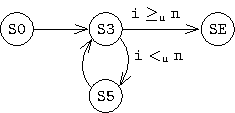
\includegraphics[scale=1.4]{chapters/figures/figMallocSpecCfg.pdf}}
\vspace{15pt}
\end{center}
\caption{\label{fig:llAllocSpecIRCFG}CFG of \SpecL{} program}
\end{subfigure}%
&
\begin{subfigure}[b]{0.5\textwidth}
\begin{center}
{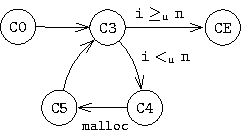
\includegraphics[scale=1.4]{chapters/figures/figMallocCCfg.pdf}}
\end{center}
\caption{\label{fig:llAllocCCFG}CFG of C program}
\end{subfigure}%
\\
\end{tabular}
\caption{\label{fig:mallocSpecCFGAndCCFG}CFG representation of Spec and C IRs shown in \cref{fig:llAllocSpecIR,fig:llAllocCIR} for the {\tt mk\_list} procedures in \cref{fig:llAllocSpec,fig:llAllocC} respectively.}
\end{figure}


Consequently, we are interested in proving that given $\sv{n} = \cv{n}$ at the procedure entries,
$\sv{ret} \indEq{} \lifted{list}{\mem{}}{lnode}{\cv{ret}}$ holds at the exits of both procedures.
Before going into the proof method,
we first introduce an alternate representation of IR, called the Control-Flow Graph (CFG for short).
\Cref{fig:llAllocSpecIRCFG,fig:llAllocCCFG} show the CFG representation of the \SpecL{} and C IRs
in \cref{fig:llAllocSpecIR,fig:llAllocCIR} respectively.
The CFG representation is fundamentally a labeled transition system representation of the corresponding IR,
and is further explored in \cref{sec:ir}.
In essence, each node represents a PC location of its IR, and each edge represents (possibly conditional)
transition between PCs through instruction execution.
For brevity, we often represent a sequence of instructions with a single edge, e.g.,
in \cref{fig:llAllocCCFG}, the edge \cpath{5,3} represents the path \cpath{5,6,7,8,3} in \cref{fig:llAllocCIR}.

\begin{figure}[H]
\begin{tabular}{cc}
\begin{subfigure}[b]{1\textwidth}
\begin{center}
{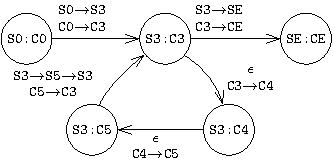
\includegraphics[scale=1.2]{chapters/figures/figMallocProductCfg.pdf}}
\end{center}
\end{subfigure}%
\end{tabular}
\caption{\label{fig:llAllocProductCFG}Product-CFG between \cref{fig:llAllocSpecIRCFG,fig:llAllocCCFG}}
\end{figure}


A common approach for showing equivalence between a pair of procedures involve finding a
bisimulation relation across the said procedure-pair.
Intuitively, a bisimulation relation (a) correlates program transitions across the specification
and implementation procedures, and (b) asserts inductively-provable invariants between
the machine states of the two procedures at the endpoints of each correlated transition \cite{pnueli98}.
Bisimulation itself can be represented as a program, called a {\em product program} \cite{covac}
and its CFG representation is called a {\em product}-CFG.
\Cref{fig:llAllocProductCFG} shows a product-CFG between the \SpecL{} and C {\tt mk\_list} procedures
in \cref{fig:llAllocSpecIRCFG,fig:llAllocCCFG} respectively.

\begin{table}[H]
\begin{center}
\caption{\label{tab:llproductInv}Node Invariants for Product-CFG in \cref{fig:llAllocProductCFG}}
\setlength{\belowcaptionskip}{-30pt}
\begin{footnotesize}
\begin{tabular}{|c|llll|}
\hline
\tt PC-Pair & \multicolumn{4}{c|} {\tt Invariants} \\
\hline
\hline
${\tt (S0:C0)}$ &
\multicolumn{4}{l|} {\Tstrut ${\tt { \circled{P}}\  n_{S}=n_{C}}$} \\
${\tt (S3:C3)}$ &
\Tstrut  ${\tt {\scriptsize \circled{I1}}\  n_{S}=n_{C}}$ & ${\tt {\scriptsize \circled{I2}}\  i_{S}=i_{C}}$ & ${\tt {\scriptsize \circled{I3}}\  i_{S} \leq_{u} n_{S}}$ & ${\tt {\scriptsize \circled{I4}}\  l_{S}\indEq{}Clist^{lnode}_{m}(l_{C})}$ \\
${\tt (S3:C4)\ (S3:C5)}$ &
\Tstrut  ${\tt {\scriptsize \circled{I5}}\  n_{S}=n_{C}}$ & ${\tt {\scriptsize \circled{I6}}\  i_{S}=i_{C}}$ & ${\tt {\scriptsize \circled{I7}}\  i_{S} <_{u} n_{S}}$ & ${\tt {\scriptsize \circled{I8}}\  l_{S}\indEq{}Clist^{lnode}_{m}(l_{C})}$ \\
${\tt (SE:CE)}$ &
\multicolumn{4}{l|} {\Tstrut  ${\tt {\circled{E}}\  ret_{S}\indEq{}Clist^{lnode}_{m}(ret_{C})}$} \\
\hline
\end{tabular}
\end{footnotesize}
\end{center}
\end{table}


At each node of the product-CFG, {\em invariants} relate the states of the \SpecL{} and C procedures respectively.
\Cref{tab:llproductInv} lists invariants for the product-CFG in \cref{fig:llAllocProductCFG}.
At the start node (\scpc{0}{0}) of the product-CFG, the precondition (labeled \circled{\small P})
ensures equality of input arguments \sv{n} and \cv{n} at the procedure entries.
Inductive invariants (labeled \circled{I}) need to be inferred at
each intermediate product-CFG node (e.g., (\scpc{3}{3})) relating both programs' states.
For example, at node (\scpc{3}{5}), \circled{\small I6} $\sv{i} = \cv{i}$ is an inductive invariant.
The inductive invariant \circled{\small I4} $\sv{l} \indEq{} \lifted{list}{\mem{}}{lnode}{\cv{l}}$
is another example of a \recursiveRelation{} and asserts equality between the intermediate \SpecL{} and C lists
at their respective loop heads.
Assuming that the precondition (\circled{\small P}) holds at the entry node (\scpc{0}{0}),
a bisimulation check involves checking that the inductive invariants hold too,
and consequently the postcondition (\circled{\small E}) holds at the exit node (\scpc{E}{E}).
Checking correctness of a bisimulation relation involves checking whether an invariant holds (along with many other things).
These checks result in proof queries which must be discharged by a solver (aka theorem prover).

\section{Our Contributions}
\label{sec:contribs}
As previously summarized in \cref{sec:motivatingexample}, an algorithm to find a bisimulation based proof of equivalence
between a \SpecL{} and C procedure involves three major algorithms:
\curved{A1} An algorithm for construction of a product-CFG by correlating program executions
across the \SpecL{} and C programs respectively.
\curved{A2} An algorithm for identification of inductively-provable invariants at intermediate correlated PCs.
\curved{A3} An algorithm for solving proof obligations generated by \curved{A1} and \curved{A2} algorithms.
Next we list our major contributions.

\begin{itemize}
\item Proof Discharge Algorithm: Solving proof obligations (\curved{A3}) involving \recursiveRelations{}
(generated by \curved{A1} and \curved{A2}) is quite interesting and forms our primary contribution.
We describe a {\em sound} proof discharge algorithm capable of tackling proof obligations involving
\recursiveRelations{} using off-the-shelf SMT solvers. Our proof discharge algorithm is also capable of
reconstruction of counterexamples for the original proof query from models returned by the individual SMT queries.
These counterexamples form the foundation of counterexample-guided heuristics for \curved{A1} and \curved{A2} algorithms
as we will see soon.
As part of our proof discharge algorithm,
we reformulate equality of ADT values (i.e. \recursiveRelations{}) as equivalence of programs
and discharge these proof queries using a nested (albeit much simpler) equivalence check.

\item Spec-to-C Automatic Equivalence Checker Tool: Our second contribution is \toolName{}, a {\em sound} equivalence checker tool
capable of proving equivalence between a \SpecL{} and a C program automatically.
\toolName{} either successfully finds a bisimulation relation implying equivalence or it provides a (sound but incomplete) unknown verdict.
\toolName{} is based on the Counter tool\cite{oopsla20} and uses specialized versions of (a) counterexample-guided correlation algorithm for
incremental construction of a product-CFG (\curved{A1}) and (b) counterexample-guided invariant inference algorithm
for inference of inductive invariants at correlated PCs in the (partially constructed) product-CFG (\curved{A2}).
\toolName{} discharges required verification conditions (i.e. proof obligations) using our Proof Discharge Algorithm.
The counterexamples generated by the proof discharge algorithm help steer the search algorithms \curved{A1} and \curved{A2}.
\end{itemize}

\section{Organization of the Thesis}
\label{sec:outline}
TODO

The rest of this thesis is divided into five chapter.
We begin with a thorough presentation of the topics discussed till now.
This includes our \SpecL{} language, the logical representation along with
bisimulation in the context of equivalence checking.
We finish with a discussion on the generated proof obligations and their language.

The next chapter illustrates our proof discharge algorithm using multiple \SpecL{} and C
sample programs.

Next, we give a detailed description of our automatic \SpecL{}-to-C equivalence checker tool \toolName{}
along with its most crucial components.

We finish with a comprehensive evaluation of \toolName{} and note its limitations.
We conclude our work by reiterating the key ideas presented alongside some related work.
\chapter{Preliminaries}
\label{sec:prelims}

\section{The Specification Language : \SpecL{}}
\label{sec:speclang}
We start with an introduction to our specification language, called \SpecL{}.
\SpecL{} supports recursive algebraic data types (ADT) \cite{algebraicdatatypes} similar to the ones available in functional languages such as Haskell \cite{marlow2010haskell} and SML \cite{standardmlspec}.
\SpecL{} does not support universal types but does allow ADTs which are mutually recursive.
Additionally, \SpecL{} is equipped with the following {\em scalar} types: \type{unit}, \type{bool} (boolean) and \type{i<N>} (fixed-width bitvectors).
ADTs can be thought of as `sum of product' types where each {\em data constructor} represents a variant (of the sum-type)
and the arguments to each data constructor represents its {\em fields} (of the product-type).
For example, the \type{List} type (defined at \apc{0} in \cref{fig:llAllocSpec}) has two variants \cons{LNil} and \cons{LCons}.
\cons{LNil} has no fields while \cons{LCons} has two fields \field{val} and \field{tail} of types \type{i32} and \type{List} respectively.
Additionally, \SpecL{} follows {\em equirecursive} typing rules i.e.
a \type{List} value $l$ and $\cons{LCons}(1_\type{i32}, l)$ have {\em equal} types.
Later in \cref{sec:valuegraph}, we further expand on ADTs in the context of a graphical representation of types and values.
The language also borrows its expression grammar heavily from functional languages.
This includes {\tt let-in}, {\tt if-then-else}, {\tt match} and function application.
Pattern matching (i.e. deconstruction) of ADT values is archieved through {\tt match}.
Unlike functional languages, \SpecL{} only supports first order functions.
Also, \SpecL{} does not support partial function application.
Hence, we constrain our attention to C programs containing only first order functions.
\SpecL{} is equipped with a special {\tt assuming-do} construct for explicitly providing assertions.
\SpecL{} also provides intrinsic scalar operators for expressing computation in C succintly yet explicitly.
Examples of scalar operators include (a) logical operators (e.g., {\tt and}), (b) bitvector arithmatic operators (e.g., {\tt bvadd(+)}),
and (c) relational operators for comparing bitvectors interpreted as unsigned or signed integers (e.g., {\tt $\leq_{\tt u,s}$}).
The equality operator ($=$) is only supported for scalar types.

\begin{figure}[H]
\begin{small}
\begin{tabular}{rcl}
\nonTerm{expr} & $\rightarrow$ & \term{if} \nonTerm{expr} \term{then} \nonTerm{expr} \term{else} \nonTerm{expr} \\
& $|$ & \term{let} \nonTerm{id} \term{=} \nonTerm{expr} \term{in} \nonTerm{expr} \\
& $|$ & \term{match} \nonTerm{expr} \term{with} \nonTerm{match-clause-list} \\
& $|$ & \term{assuming} \nonTerm{expr} \term{do} \nonTerm{expr} \\
& $|$ & \nonTerm{id} \term{(} \nonTerm{expr-list} \term{)} \\
& $|$ & \nonTerm{data-cons} \term{(} \nonTerm{expr-list} \term{)} \\
& $|$ & \nonTerm{expr} \term{is} \nonTerm{data-cons} \\
& $|$ & \nonTerm{expr} \nonTerm{scalar-op} \nonTerm{expr} \\
& $|$ & \nonTerm{literal$_{\mathrm{Unit}}$} $|$ \nonTerm{literal$_{\mathrm{Bool}}$} $|$ \nonTerm{literal$_{\mathrm{i<N>}}$} \\
\\
\nonTerm{match-clause-list} & $\rightarrow$ & \nonTerm{match-clause}$^*$ \\
\nonTerm{match-clause} & $\rightarrow$ & \term{$|$} \nonTerm{data-cons} \term{(} \nonTerm{id-list} \term{)} \term{$\Rightarrow$} \nonTerm{expr} \\
\nonTerm{expr-list} & $\rightarrow$ & \term{$\epsilon$} \term{$|$} \nonTerm{expr} \term{,} \nonTerm{expr-list} \\
\nonTerm{id-list} & $\rightarrow$ & \term{$\epsilon$} \term{$|$} \nonTerm{id} \term{,} \nonTerm{id-list} \\
\\
\nonTerm{literal$_{\mathrm{Unit}}$} & $\rightarrow$ & \term{()} \\
\nonTerm{literal$_{\mathrm{Bool}}$} & $\rightarrow$ & \term{false} $|$ \term{true} \\
\nonTerm{literal$_{\mathrm{i<N>}}$} & $\rightarrow$ & [\term{0$\dots$2$^{\mathrm{N}}$-1}] \\
\end{tabular}
\end{small}
\caption{\label{fig:specgrammar}Simplified expression grammar of \SpecL{} language}
\end{figure}

\Cref{fig:specgrammar} shows the simplified expression grammar for \SpecL{} language.
\nonTerm{data-cons} represents a ADT data constructor.
The `\nonTerm{expr} {\tt is} \nonTerm{data-cons}' construct returns a \type{bool} and is used to test whether the top-level constructor
of the ADT value \nonTerm{expr} is \nonTerm{data-cons}.
\nonTerm{scalar-op} includes the logical, arithmatic and relational operators supported by \SpecL{}.

\begin{figure}
\begin{tabular}{cc}
\begin{subfigure}[b]{0.45\textwidth}
\begin{center}
\begin{allLangEnvFoot}
~{\scriptsize \textcolor{mygray}{   }}~   
~{\scriptsize \textcolor{mygray}{S0:}}~ i32 sum_list (List l) {
~{\scriptsize \textcolor{mygray}{S1:}}~   i32 sum $\coloneqq$ ${\tt 0_{i32}}$;
~{\scriptsize \textcolor{mygray}{S2:}}~   while $\mathrm{\tt\neg (l\ is\ LNil)}$:
~{\scriptsize \textcolor{mygray}{S3:}}~     // (l is LCons);
~{\scriptsize \textcolor{mygray}{S4:}}~     sum $\coloneqq$ sum + ${\tt l.val}$;
~{\scriptsize \textcolor{mygray}{S5:}}~     l   $\coloneqq$ l.next;
~{\scriptsize \textcolor{mygray}{S6:}}~   return sum;
~{\scriptsize \textcolor{mygray}{SE:}}~ }
\end{allLangEnvFoot}
\end{center}
\caption{\label{fig:llTraverseSpec}(Abstracted) Spec IR}
\end{subfigure}%
&
\begin{subfigure}[b]{0.55\textwidth}
\begin{center}
\begin{allLangEnvFoot}
~{\scriptsize \textcolor{mygray}{\ \ \ }}~ unsigned sum_list (lnode* l);
~{\scriptsize \textcolor{mygray}{C0:}}~ i32 sum_list (i32 l) {
~{\scriptsize \textcolor{mygray}{C1:}}~   i32 sum $\coloneqq$ ${\tt 0_{i32}}$;
~{\scriptsize \textcolor{mygray}{C2:}}~   while ${\tt l \neq 0_{i32}}$:
~{\scriptsize \textcolor{mygray}{C3:}}~     sum $\coloneqq$ sum + $\structPointer{\tt l}{m}{\tt lnode}{val}$;
~{\scriptsize \textcolor{mygray}{C4:}}~     l   $\coloneqq$ $\structPointer{\tt l}{m}{\tt lnode}{next}$;
~{\scriptsize \textcolor{mygray}{C5:}}~   return sum;
~{\scriptsize \textcolor{mygray}{CE:}}~ }
\end{allLangEnvFoot}
\end{center}
\caption{\label{fig:llTraverseC}(Abstracted) C IR}
\end{subfigure}%
\\
\begin{subfigure}[b]{0.45\textwidth}
\begin{center}
{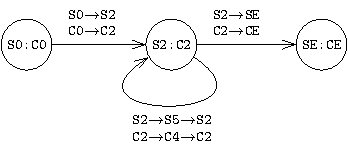
\includegraphics[scale=1.1]{chapters/figures/figSumListProductCfg.pdf}}
\end{center}
\caption{\label{fig:llTraverseProduct}Product-CFG}
\end{subfigure}%
&
\begin{subfigure}[b]{0.55\textwidth}
\begin{center}
\begin{footnotesize}
\begin{tabular}{|c|l|}
\hline
\tt PC-Pair & \multicolumn{1}{c|} {\tt Invariants} \\
\hline
\hline
${\tt (S0:C0)}$ &
\Tstrut ${\tt {\circled{P}}\  l_{S}\indEq{}Clist^{lnode}_{m}(l_{C})}$ \\
\multirow{2}{*}{${\tt (S2:C2)}$} &
\Tstrut \Bstrut ${\tt {\scriptsize \circled{I1}}\  l_{S}\indEq{}Clist^{lnode}_{m}(l_{C})}$ \\ & ${\tt {\scriptsize \circled{I2}}\  sum_{S}=sum_{C}}$ \\
${\tt (SE:CE)}$ &
\Tstrut \Bstrut ${\tt {\circled{E}}\  ret_{S}=ret_{C}}$ \\
\hline
\end{tabular}
\end{footnotesize}
\vspace{13px}
\end{center}
\caption{\label{fig:llTraverseProductInv}Node Invariants of the Product-CFG}
\end{subfigure}%
\\
\end{tabular}
\caption{\label{fig:llTraverseSpecAndC}Spec and C programs for traversing a linked list. \Cref{fig:llTraverseProduct} shows the Product-CFG between the IRs in \cref{fig:llTraverseSpec,fig:llTraverseC}. The inductive invariants of the Product-CFG are given in \cref{fig:llTraverseProductInv}.}
\end{figure}

\begin{figure}
\begin{tabular}{cc}
\begin{subfigure}[b]{0.45\textwidth}
\begin{center}
\begin{allLangEnvFoot}
~{\scriptsize \textcolor{mygray}{S0:}}~ i32 sum_list (List l) {
~{\scriptsize \textcolor{mygray}{S1:}}~   i32 sum $\coloneqq$ ${\tt 0_{i32}}$;
~{\scriptsize \textcolor{mygray}{S2:}}~   while $\neg$(l is LNil):
~{\scriptsize \textcolor{mygray}{S3:}}~     // (l is LCons);
~{\scriptsize \textcolor{mygray}{S4:}}~     sum $\coloneqq$ sum + l.val;
~{\scriptsize \textcolor{mygray}{S5:}}~     l   $\coloneqq$ l.next;
~{\scriptsize \textcolor{mygray}{S6:}}~   return sum;
~{\scriptsize \textcolor{mygray}{SE:}}~ }
\end{allLangEnvFoot}
\end{center}
\caption{\label{fig:llTraverseSpecIR}(Abstracted) Spec IR}
\end{subfigure}%
&
\begin{subfigure}[b]{0.55\textwidth}
\begin{center}
\begin{allLangEnvFoot}
~{\scriptsize \textcolor{mygray}{C0:}}~ i32 sum_list (i32 l) {
~{\scriptsize \textcolor{mygray}{C1:}}~   i32 sum $\coloneqq$ ${\tt 0_{i32}}$;
~{\scriptsize \textcolor{mygray}{C2:}}~   while ${\tt l \neq 0_{i32}}$:
~{\scriptsize \textcolor{mygray}{C3:}}~     sum $\coloneqq$ sum + $\structPointer{\tt l}{\mem{}}{lnode}{val}$;
~{\scriptsize \textcolor{mygray}{C4:}}~     l   $\coloneqq$ $\structPointer{\tt l}{\mem{}}{lnode}{next}$;
~{\scriptsize \textcolor{mygray}{C5:}}~   return sum;
~{\scriptsize \textcolor{mygray}{CE:}}~ }
\end{allLangEnvFoot}
\vspace{7px}
\end{center}
\caption{\label{fig:llTraverseCIR}(Abstracted) C IR}
\end{subfigure}%
\\
\begin{subfigure}[b]{0.45\textwidth}
\begin{center}
{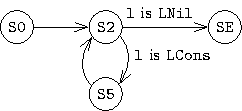
\includegraphics[scale=1.3]{chapters/figures/figSumListSpecCfg.pdf}}
\end{center}
\caption{\label{fig:llTraverseSpecCFG}CFG of \SpecL{} Program}
\end{subfigure}%
&
\begin{subfigure}[b]{0.55\textwidth}
\begin{center}
{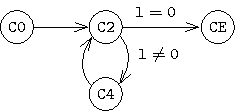
\includegraphics[scale=1.3]{chapters/figures/figSumListCCfg.pdf}}
\end{center}
\caption{\label{fig:llTraverseCCFG}CFG of C Program}
\end{subfigure}%
\\
\end{tabular}
\caption{\label{fig:llTraverseSpecAndCIRAndCFG}IRs and CFGs of the \SpecL{} and C Programs in \cref{fig:llTraverseSpec,fig:llTraverseC} respectively.}
\end{figure}


\section{Abstract Representation of Programs}
\label{sec:ir}
As outlined in \cref{sec:motivatingexample}, we convert both \SpecL{} and C programs to a common
abstract representation called the {\em Control Flow Graph} (CFG for short).
This process involves converting both programs to a linear representation called the IR.
This section presents both IR and CFG representations for the original \SpecL{} and C programs.

\subsection{Conversion of Programs to their Intermediate Representation}
\label{sec:irconv}
IR is a Three-Address-Code (3AC) style intermediate representation.
We often omit intermediate registers in the IR for brevity, and refer to this as the {\em abstracted} IR.
We have already seen the IRs (in \cref{fig:llAllocSpecIR,fig:llAllocCIR}) for the \SpecL{} and C programs
that construct lists in \cref{fig:llAllocSpec,fig:llAllocC}.
\Cref{fig:llTraverseSpec,fig:llTraverseC} show \SpecL{} and C programs that traverse a list of integers
and return the sum of all the values in it.
The corresponding IR programs for the above are shown in \cref{fig:llTraverseSpecIR,fig:llTraverseCIR}.

The following major steps are performed during conversion of a \SpecL{} source to its IR representation:

\begin{enumerate}
\item {\tt match} statements are converted to explicit {\tt if-else} conditionals where each branch is
associated with a {\tt match} branch. The {\em sum-is} operator is used in the condition to query
the top-level data constructor of an expression. The fields of the data constructor are bound to
variables using the {\em product-access} or {\em accessor} operator.
For example, the {\tt match} statement in \apc{3} (in \cref{fig:llTraverseSpec}) is lowered to {\tt if-else}
in \cref{fig:llTraverseSpecIR}, where `\sumIs{\comv{l}}{LCons}' is used to test whether \comv{l} is
of kind \cons{LCons} and `\prodAccess{\comv{l}}{val}' is used to extract the \field{val} field of \cons{LCons} data constructor.
Importantly, the expression `\prodAccess{e}{fi}' is well-formed iff `\sumIs{e}{\mathnormal{V}_{fi}}', where $V_\field{fi}$ represents the
data constructor containing the field \field{fi}.
The construction of the IR guarantees the well-formedness of all expressions.
\item All tail-recursive calls are converted to loops in the IR. However, all non-tail procedure calls are preserved as is.
This transformation enables direct correlation (during equivalence checking) of tail-recursion in \SpecL{} with native loops in C.
For example, the tail recursive function {\tt sum\_list\_impl} in \apc{2} (in \cref{fig:llTraverseSpec}) is converted to a non-recursive function with a loop.
\item All {\em helper} functions\footnote{We use a special marker to designate a function as `helper' in \SpecL{}.
For simplicity, this marker is omitted and instead helper function names are ended with the `{\tt \_impl}' suffix.}
are inlined at their call-site.
We are only interested in proving equivalence of non-helper functions in \SpecL{} with their C counterparts.
For example, the helper function {\tt sum\_list\_impl} (now non-recursive due to previous step), is inlined
at call-site \apc{7} in \cref{fig:llTraverseSpec}.
\end{enumerate}

Similarly, the following transformations are carried out during conversion of a C source to its IR:

\begin{enumerate}
\item Non-determinism in the original C program is determinized in the IR.
This includes concretizing the size and memory layouts of both scalar (e.g. \type{int})
and compound (e.g., \type{struct}) types, along with fixing the order of evaluation in case
it is unspecified.
For example, during conversion of C program in \cref{fig:llAllocC} to IR (in \cref{fig:llAllocCIR}),
the sizes of pointer and \type{unsigned} types are fixed to 32 bits (i.e. \type{i32}).
Similarly, the memory layout (including alignment and offset) of \type{lnode} struct defined in \bpc{0} (in \cref{fig:llAllocC}) is chosen.
The implications of determinizing the C program behaviour are further discussed in \cref{sec:spectocalgo}.
For now, it is sufficient to note that we are interested in equivalence between \SpecL{} and this determinized version of C.
\item The memory state of the C program is made explicit, represented using the byte-addressable array `\mem{}'.
Memory loads and stores are represented using explicit operations on \mem{}, e.g.,
(a) memory load in \cpc{3} in \cpc{4} in \cref{fig:llTraverseCIR}, and
(b) memory stores in \cpc{5} and \cpc{6} in \cref{fig:llAllocCIR}.
The memory load and store operators are defined promptly in \cref{sec:irops}
\item We annotate calls to memory allocation functions (e.g., {\tt malloc}) with their call-site.
For example, {\tt malloc$_\cpc{4}$} is annotated with its call-site \cpc{4} in \cref{fig:llAllocCIR}.
These annotations are used by a points-to analysis done as part of our equivalence checking procedure,
and defined subsequently in \cref{sec:pointsToFormal}.
\end{enumerate}

\subsection{IR Instructions}
\label{sec:irops}
Note that both \SpecL{} and C programs are converted to the common IR.
On the \SpecL{} side, IR supports scalar as well as ADT types defined in the \SpecL{} program under consideration.
The IR also inherits the scalar operators available as part of \SpecL{}.
Each ADT value can be thought of as a key-value dictionary that maps each of its field names
to their respective values.
These key-value pairs are accessed using the previously introduced {\em accessor} operator,
e.g., \prodAccess{l}{val} and \prodAccess{l}{next} represents the first and second fields of the
\cons{LCons} data constructor in \cref{fig:llTraverseSpecIR}.
Recall that, the IR also allows querying the top-level variant of an ADT value using the
{\em sum-is} operator, e.g., \sumIs{l}{LNil} in \cref{fig:llTraverseSpecIR}.
The \field{val} field is associated with the \cons{LCons} data constructor and
evidently, \prodAccess{l}{val} (and \prodAccess{l}{next}) is only {\em well-formed} under \sumIs{l}{LCons}.
As discussed, the well-formedness of all {\em accessor} expressions are preserved during
construction of IR for a \SpecL{} program.
Using {\em accessor} and {\em sum-is} operators, a \type{List} value $l$ can be expanded as:

\begin{equation}
\label{eqn:specDeconstruct}
U_S: l = \sumIf{\sumIs{l}{LNil}} \  \sumThen{\cons{LNil}} \  \sumElse{\cons{LCons}(\prodAccess{l}{val}, \prodAccess{l}{next})}
\end{equation}

In this expanded representation of $l$,
the {\em sum-deconstruction} operator `\sumDtor{}'
conditionally deconstructs the sum type into its variants \cons{LNil} and \cons{LCons}.
The {\em underlined} \sumDtor{} operator is a stricter version of {\tt if-then-else}, and is only used for ADT values.
An \sumDtor{} expression $e$ (for an ADT type $T$) must satisfy the following properties:
(a) $e$ has exactly one branch for each data construction of $T$ (in the order they are defined),
and (b) the branch associated with the data constructor $V$ has the form $V(e_1,e_2,\dots)$ i.e. its top-level operator is $V$.
For example, an \sumDtor{} expression for the \type{List} type must be of the form:
`\sumIf{e_1} \sumThen{\cons{LNil}} \sumElse{\cons{LCons}(e_2,e_3)}' for some expressions $e_1,e_2,e_3$.
\Cref{eqn:specDeconstruct} is called the {\em unrolling procedure} for the \type{List} variable $l$.
We can similarly define the unrolling procedure for any ADT variable (based on the definition of the ADT).

On the C side, the size of a pointer is fixed\footnote{We choose an address width of 4 bytes or 32 bits for our evaluation.}
and the memory state is modeled as a byte-addressable array over bitvectors (represented by \mem{}).
``\memRead{\mem{}}{p}{T}'' represents a memory load operation and is equal to the bytes
at addresses [$p$, $p$+\sizeof{T}) in \mem{}, interpreted as a value of type \type{T}.
Similarly, ``\memWrite{\mem{}}{p}{v}{T}'' represents a memory store operation and is equal to \mem{}
everywhere except at addresses [$p$, $p$+\sizeof{T}) which contains
the value $v$ of type \type{T} (e.g., \cpc{5} in \cref{fig:llAllocCIR}).
We use the following two C-like syntaxes to represent more intricate memory loads succintly:

\begin{enumerate}
\item ``\structPointer{p}{\mem{}}{T}{fi}'' is equivalent to ``\memRead{\mem}{p+\offsetof{T}{fi}}{\typeof{T.fi}}''
i.e., it returns the bytes in the memory array \mem{} starting at address `$p+\offsetof{T}{fi}$'
and interpreted as a value of type \typeof{T.fi}.

\item ``\arrIndex{p}{i}{\mem{}}{T}'' is equivalent to ``\memRead{\mem}{p+i \times \sizeof{T}}{T}''
i.e., it returns the bytes in the memory array \mem{} starting at address `$p+i \times \sizeof{T}$'
and interpreted as a value of type \type{T}.
Interestingly, $\memRead{\mem{}}{p}{T} = \arrIndex{p}{0}{\mem{}}{}$.
\end{enumerate}

Recall that the size and layout of each type in C is concretized in the IR,
and hence the values `\offsetof{T}{f}' and `\sizeof{T}' are constants.
We use the `\addrof{}' operator to extract the address of a memory load expression:
``\addrof{\memRead{\mem{}}{p}{T}}'' is equivalent to $p$.
For example, at PC \cpc{5} in \cref{fig:llAllocCIR}, $\addrof{\structPointer{\mathnormal{p}}{\mem{}}{lnode}{val}} \Leftrightarrow p+\offsetof{lnode}{val}$.
Additionally, given a bitvector expression $e$, ``$e{\tt [ub:lb]}$'' represents a bitvector extract operation that extracts the bits
in the range [lb,ub] from $e$ resulting in a $(ub-lb+1)$-sized bitvector expression.

\subsection{Control-Flow Graph Representation}
\Cref{fig:llTraverseSpecCFG,fig:llTraverseCCFG} show the Control-Flow Graph (CFG) representation
of the \SpecL{} and C IRs in \cref{fig:llTraverseSpecIR,fig:llTraverseCIR} respectively.
The Control-Flow Graph is an alternate graphical representation of an IR program that emphasizes
the control flow structures of the static program.
Each CFG node represents a program point (i.e. IR PC) and is denoted by $n$.
The CFG representation is analogous to a deterministic labeled transition systems and
uses a symbolic state $\Omega_n$ to represent the machine state at node $n$.
An edge from $n$ to $n'$ (denoted by $\omega[n \rightarrow n']$) represents transition
from $n$ to $n'$ through execution of instructions and is associated with:

\begin{enumerate}
\item An {\em edge condition} representing the condition that must be satisfied by $\Omega_n$
to trigger the edge $\omega$.
\item A {\em transfer function} representing the symbolic state at $n'$ ($\Omega_{n'}$) as a function of $\Omega_n$
i.e. how the machine state is mutated along the edge $\omega$.
\item An {\em UB condition} representing the condition that must be satisfied by $\Omega_n$ for
the transition $\omega$ to be well-defined. For a \SpecL{} function, assertions expressed
using the {\tt assuming-do} statement form the UB assumptions.
\end{enumerate}

For brevity, we often represent a sequence of instructions with a single edge, e.g.,
in \cref{fig:llAllocCCFG}, the edge \cpath{5,3} represents the path \cpath{5,6,7,8,3}.
In such a case, the transfer function of the edge is the composition of the sequence of instructions.
A CFG must contain exactly one entry node (representing the entry to the function), but may contain
multiple exit nodes (each representing an exit from the function).
An edge incident on an exit node is called an {\em exit edge} and is associated with an {\em action} representing
the values returned as a function of the symbolic state at the source node.
Actions form the observable behaviour of a CFG while transition through non-exit edges are internal to the program.
Additionally, exit edges are always associated with an edge condition of {\tt true} and an identity transfer function.
Recall that for a C CFG, the action includes both the returned value (if non-void) and the memory state.
We omit these transfer functions in the CFG figures (as they are shown in their corresponding IR)
and only show the edge conditions (unless they are {\em true}).
Henceforth, we refer to the CFGs of \SpecL{} and C functions as \sprog{} and \cprog{} respectively.

\section{Equivalence Definition}
\label{sec:eqdef}
Given (1) a \SpecL{} function specification \sprog{}, (2) a C implementation \cprog{},
(3) a precondition \pre{} that relates the initial inputs \sv{Input} and \cv{Input} to
\sprog{} and \cprog{} respectively, and (4) a postcondition \post{} that relates the final outputs
\sv{Output} and \cv{Output} of \sprog{} and \cprog{} respectively\footnote{\cv{Input} and \cv{Output}
include the initial and final memory state of \cprog{} respectively.}:
\sprog{} and \cprog{} are {\em equivalent} if for all possible inputs \sv{Input} and \cv{Input} such that
$\pre{}(\sv{Input},\cv{Input})$ holds,
\sprog{}'s execution is well-defined on \sv{Input}, {\em and}
\cprog{}'s memory allocation requests during its execution on \cv{Input} are successful,
then both programs \sprog{} and \cprog{} produce outputs such that $\post{}(\sv{Output},\cv{Output})$ holds.
$$
\pre{}(\sv{Input},\cv{Input}) \land \sdef{} \land \cfits{} \Rightarrow \post{}(\sv{Output},\cv{Output})
$$

The \sdef{} antecedent states that we are only interested in proving equivalence for
well-defined executions of \sprog{}, i.e., executions that satisfy all assertions expressed
using the {\tt assuming-do} statement.
The \cfits{} antecedent states that we prove equivalence under the assumption that \cprog{}'s memory
requirements fit within the available system memory i.e., only for those executions of \cprog{}
in which all memory allocation requests (through {\tt malloc} calls) are successful.

Recall that the observables of \sprog{} and \cprog{} are the actions associated with their exit edges (i.e. returned values).
For \sprog{}, observables include the explicit value returned.
For \cprog{}, observables include the returned value alongside the memory state at program exit.
The postcondition \post{} relates these outputs of the two programs.
The pair $(\pre{},\post{})$ represents the input-output behaviour of \cprog{} in terms of the specification \sprog{},
and is called the {\em input-output specification}.
In general, \SpecL{} and C sources may contain multiple top-level procedures, with calls to each other.
In this case, we are interested in finding equivalence between each pair
of \sprog{} and \cprog{} procedures with respect to their input-output specification.

Sometimes, the user may be interested in constraining the nature of inputs to \cprog{}
for the purpose of checking equivalence only for {\em well-defined} inputs.
In those circumstances, we use a combination of \pre{} and \sdef{} to constrain
the execution of \cprog{} to inputs for which we are interested in proving equivalence.
For example, the C library function {\tt strlen(\type{char}* \cv{str})} is well-defined only if \cv{str}
represents a valid null character terminated string.
This includes the assumption that the pointer \cv{str} may not be null.
Since \SpecL{} has no notion of pointers, we expose this conditional well-definedness of C strings
through an explicit constructor e.g. \cons{SInvalid} for the \type{String} ADT defined as:
$$
\type{Str} = \cons{SInvalid}\ |\ \cons{SNil}\ |\ \cons{SCons}(\type{i8}, \type{Str})
$$
\sdef{} asserts $\neg(\sumIs{\sv{str}}{SInvalid})$ (using {\tt assuming-do}) and
the precondition \pre{} contains the relation $(\sumIs{\sv{str}}{SInvalid}) \Leftrightarrow (\cv{str}=0)$.
Hence, \sdef{} and \pre{} ensure that we compute equivalence for those
executions of \sprog{} and \cprog{} where the input strings are well-defined.
A similar strategy is employed for other functions as explored later in \cref{sec:results}.

\begin{figure}
\begin{tabular}{cc}
\begin{subfigure}[b]{0.45\textwidth}
\begin{center}
{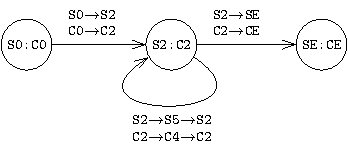
\includegraphics[scale=1.1]{chapters/figures/figSumListProductCfg.pdf}}
\end{center}
\caption{\label{fig:llTraverseProduct}Product-CFG}
\end{subfigure}%
&
\begin{subfigure}[b]{0.55\textwidth}
\begin{center}
\begin{footnotesize}
\begin{tabular}{|c|l|}
\hline
{\bf PC-Pair} & \multicolumn{1}{c|} {\bf Invariants} \\
\hline
\hline
(\scpc{0}{0}) &
\Tstrut $\circled{P}\  \sv{l} \indEq{} \lifted{list}{\mem{}}{lnode}{\cv{l}}$ \\
\multirow{2}{*}{(\scpc{2}{2})} &
\Tstrut $\circled{\scriptsize I1}\  \sv{l} \indEq{} \lifted{list}{\mem{}}{lnode}{\cv{l}}$ \\ &
\Tstrut $\circled{\scriptsize I2}\  \sv{sum} = \cv{sum}$ \\
(\scpc{E}{E}) &
\Tstrut $\circled{\scriptsize E}\  \sv{ret} = \cv{ret}$ \\
\hline
\end{tabular}
\end{footnotesize}
\vspace{13px}
\end{center}
\caption{\label{fig:llTraverseProductInv}Node Invariants of the Product-CFG}
\end{subfigure}%
\\
\end{tabular}
\caption{\label{fig:llTraverseProductCFGInvs} Product-CFG between the IRs in \cref{fig:llTraverseSpec,fig:llTraverseC}. The inductive invariants of the Product-CFG are given in \cref{fig:llTraverseProductInv}.}
\end{figure}


\section{Bisimulation Relation}
\label{sec:bisim}
Recall that,
we construct a {\em bisimulation relation} to identify equivalence between the CFGs of \SpecL{} and C procedures.
A bisimulation relation correlates the transitions of \sprog{} and \cprog{} in lockstep, such that the
lockstep execution ensures identical observable behaviour.
A bisimulation relation between two programs can be represented using a {\em product program}
\cite{covac} and the CFG representation of a product program is called a {\em product}-CFG.
\Cref{fig:llTraverseProduct} shows a product-CFG, that encodes the lockstep execution
(bisimulation relation) between the CFGs in \cref{fig:llTraverseSpecCFG,fig:llTraverseCCFG}.

A node in the product-CFG is formed by pairing nodes of \sprog{} and \cprog{},
e.g., (\scpc{2}{2}) is formed by pairing \spc{2} and \cpc{2}.
If the lockstep execution of both programs is at node (\scpc{2}{2}) in the product-CFG,
then \sprog{}'s execution is at \spc{2} and \cprog{}'s execution is at \cpc{2}.
The start node (\scpc{0}{0}) of the product-CFG correlates the start nodes of CFGs of \sprog{} and \cprog{}.
Similarly, the exit node (\scpc{E}{E}) correlates the exit nodes of both programs.

An edge in the product-CFG is formed by pairing a {\em path} (a sequence of edges) in \sprog{}
with a path in \cprog{}\footnote{TODO: to keep the discussion simple, we consider paths to be sequence of edges. however, a more general approach of pathset
is used based on the Counter tool \cite{oopsla20}. We will explore pathsets in more detail later on.}.
A product-CFG edge encodes the lockstep execution of its correlated paths.
For example, the product-CFG edge \scedge{2}{2}{2}{2} is formed by pairing
\spath{2,5,2} and \cpath{2,4,2} in \cref{fig:llTraverseSpecCFG,fig:llTraverseCCFG} respectively,
and represents that when \sprog{} makes the transition \spath{2,5,2}, \cprog{} makes the transition \cpath{2,4,2}
in lockstep.
In general, a product-CFG edge $e$ may correlate a finite path \sv{\rho} in \sprog{} with a finite path
\cv{\rho} in \cprog{}, written $e=(\sv{\rho},\cv{\rho})$.
The empty path $\epsilon$ in \sprog{} may be correlated with a finite path in \cprog{},
effectively simulating a {\em stuttering bisimulation} relation.
However, a product-CFG is only well-formed (i.e. represents a valid bisimulation relation)
if no loop path in \cprog{} is correlated with $\epsilon$ in \sprog{}.
For example, \cref{fig:llAllocProductCFG} shows the product-CFG between the programs
in \cref{fig:llAllocSpecIRCFG,fig:llAllocCCFG} respectively.
The edges \scedge{3}{3}{3}{4} and \scedge{3}{4}{3}{5} correlate the empty path $\epsilon$
with the non-empty paths \cpath{3,4} and \cpath{4,5} respectively.
However, the only loop path \cpath{3,4,5,3} in \cprog{} is still correlated with the non-empty path \spath{3,5,3}
in \sprog{} and thus, the product-CFG in \cref{fig:llAllocProductCFG} satisfies this well-formedness criterion.
This well-formedness condition is required to preserve {\em divergence}, i.e. either both programs terminate or
both continue indefinitely.

At the start node (\scpc{0}{0}) of the product-CFG in \cref{fig:llTraverseProduct},
the precondition \pre{} (labeled \circled{\small P})
ensures equality of input lists \sv{l} and \cv{l} at procedure entries.
{\em Inductive invariants} (labeled \circled{I}) are inferred
at each intermediate product-CFG node (e.g., (\scpc{2}{2})) that relate
the values of \sprog{} with values and memory state of \cprog{}.
At the exit node (\scpc{E}{E}) of the product-CFG, the postcondition \post{} (labeled \circled{\small P})
represents equality of observable outputs and forms our overall proof obligation.
Assuming that the precondition \pre{} (\circled{\small P}) holds at the entry node (\scpc{0}{0}),
a bisimulation check involves checking that the inductive invariants (\circled{\small I}) hold too,
and consequently the postcondition \post{} (\circled{\small E}) holds at the exit node (\scpc{E}{E}).
The input-output specification (i.e. $(\pre{},\post{})$) is manually provided by the user
while all inductive invariants are identified by an invariant inference algorithm described in \cref{sec:invinferalgo}.

\section{Recursive Relation}
\label{sec:recrel}
In \cref{sec:motivatingexample}, we briefly introduced a lifting constructor (\lift{list}{\mem{}}{lnode})
and \recursiveRelations{}.
In \cref{fig:llTraverseProductInv}, the precondition (\circled{\small P}) is another instance
of a \recursiveRelation{}:
``\sv{l} \indEq{} \lifted{list}{\mem{}}{lnode}{\cv{l}}'' where \sv{l} and \cv{l}
represent the input arguments to the \SpecL{} and C procedures respectively,
\type{lnode} is the C \type{struct} type that contains the \field{val} and \field{next} fields (defined at \bpc{0} in \cref{fig:llTraverseC}),
and \mem{} is the byte-addressable array representing the current memory state of the C program.
$l_1 \indEq{} l_2$ is read {\em $l_1$ is recursively equal to $l_2$} and is semantically equivalent
to $l_1 = l_2$. The `\indEq{}' simply emphasizes that $l_1$ and $l_2$ are (possibly recursive) ADT values.
The lifting constructor \lift{list}{\mem{}}{lnode} `lifts' a C pointer value $p$
(pointing to an object of type \type{struct lnode}) and
memory state \mem{} to a (possibly infinite in case of a circular list) \type{List} value,
and is defined through its {\em unrolling procedure} as follows:

\begin{equation}
\label{eqn:clist}
\begin{split}
U_C:\ &\lifted{list}{\mem{}}{lnode}{p \ctype{i32}} = \sumIf{p=0} \ \sumThen{\cons{LNil}} \\ & \qquad\qquad\ \ \ \sumElse{\cons{LCons}(\structPointer{p}{\mem{}}{lnode}{val}, \lifted{list}{\mem{}}{lnode}{\structPointer{p}{\mem{}}{lnode}{next}})}
\end{split}
\end{equation}

Note the recursive nature of the lifting constructor \lift{list}{\mem{}}{lnode}: if the pointer $p$ is zero
(i.e. $p$ is a null pointer), then it represents the empty list \cons{LNil};
otherwise it represents the list formed by \cons{LCons}-ing the value stored at
\structPointer{p}{\mem{}}{lnode}{val} in memory \mem{} and the list formed by recursively
lifting \structPointer{p}{\mem{}}{lnode}{next} through \lift{list}{\mem{}}{lnode}.
\lifted{list}{\mem{}}{lnode}{p} allows us to adapt a C linked list (formed by chasing pointers
in the memory \mem{}) to a \type{List} value and compare it with a \SpecL{} \type{List}
value for equality.

\section{Proof Obligations}
\label{sec:proofobl}
As previously discussed, algorithms for (a) incremental construction of a Product-CFG
and (b) inference of invariants at intermediate PCs in the (partially constructed) product-CFG, are
based on prior work\cite{oopsla20} and discussed subsequently in \cref{sec:searchalgo,sec:invinferalgo}.
For now, we discuss the proof obligations that arise from a given product-CFG.
Recall that a bisimulation check involves checking that all inductive invariants
(and the postcondition \post{}) hold at their associated product-CFG nodes.

We use relational Hoare triples to express these proof obligations \cite{relationalHoareLogic,hoareTriple}.
If $\phi$ denotes a predicate relating the machine states of \sprog{} and \cprog{}, then
for a product-CFG edge $e=(\sv{\rho},\cv{\rho})$, \hoareTriple{\phi_s}{e}{\phi_d}
denotes the condition:
if any machine states \sv{\sigma} and \cv{\sigma} of programs \sprog{} and \cprog{} are related through
precondition $\phi_s(\sv{\sigma},\cv{\sigma})$ and the finite paths \sv{\rho} and \cv{\rho}
are executed in \sprog{} and \cprog{} respectively,
then execution terminates normally in states $\sv{\sigma}^{'}$ (for \sprog{}) and
$\cv{\sigma}^{'}$ (for \cprog{}) and postcondition $\phi_d(\sv{\sigma}^{'},\cv{\sigma}^{'})$ holds.

For every product-CFG edge $e = (s \rightarrow d) = (\sv{\rho}, \cv{\rho})$,
we are interested in proving: \hoareTriple{\phi_s}{\sv{\rho},\cv{\rho}}{\phi_d},
where $\phi_s$ and $\phi_d$ are the node invariants at the product-CFG nodes $s$ and $d$
respectively.
The weakest-precondition transformer is used to translate a Hoare triple
\hoareTriple{\phi_s}{\sv{\rho},\cv{\rho}}{\phi_d} to the following
first-order logic formula:

\begin{equation}
\label{eqn:firstOrderFormula}
(\phi_s \land {\tt pathcond}_{\sv{\rho}} \land {\tt pathcond}_{\cv{\rho}} \land {\tt ubfree}_{\sv{\rho}}) \Rightarrow {\tt WP}_{{\sv{\rho},\cv{\rho}}}(\phi_d)
\end{equation}

Here, ${\tt pathcond}_{\rho_X}$ represents the condition that path $\rho$ is taken in program $X$
and ${\tt ubfree}_{\sv{\rho}}$ represents the condition that execution of \sprog{} along path $\sv{\rho}$
is free of undefined behaviour.
${\tt WP}_{{\sv{\rho},\cv{\rho}}}(\phi_d)$ represents the weakest-precondition
of the predicate $\phi_d$ across the product-CFG edge $e = (\sv{\rho},\cv{\rho})$.
From now on, we will use `\lhs{}' and `\rhs{}' to refer to the antecedent and consequent of
the implication operator `$\Rightarrow$' in \cref{eqn:firstOrderFormula}.

For example, checking that the loop invariant \circled{\small I2}
$\sv{l} \indEq{} \lifted{list}{\mem{}}{lnode}{\cv{l}}$ holds at (\scpc{2}{2}) in \cref{fig:llTraverseProduct}
requires us to prove the following two proof obligations:
\circled{1} \hoareTriple{\scpcinv{0}{0}}{\spath{0,2},\cpath{0,2}}{\sv{l} \indEq{} \lifted{list}{\mem{}}{lnode}{\cv{l}}} and
\circled{2} \hoareTriple{\scpcinv{2}{2}}{\spath{2,5,2},\cpath{2,4,2}}{\sv{l} \indEq{} \lifted{list}{\mem{}}{lnode}{\cv{l}}}.
Using weakest precondition predicate transformer, the proof obligation \circled{2} reduces to the following first-order logic formula:

\begin{equation}
\label{eqn:firstOrderFormulaExample}
\begin{split}
\sv{l} \indEq{} \lifted{list}{\mem{}}{lnode}{\cv{l}} \land \sv{sum} = \cv{sum}
\land (\sumIs{\sv{l}}{LCons}) \land (\cv{l} \neq 0) \\ \Rightarrow
\prodAccess{\sv{l}}{next} \indEq{} \lifted{list}{\mem{}}{lnode}{\structPointer{\cv{l}}{\mem{}}{lnode}{next}}
\end{split}
\end{equation}

Due to the presence of \recursiveRelations{}, these proof queries
(e.g., \cref{eqn:firstOrderFormulaExample}) cannot be solved directly by
off-the-shelf solvers and require special handling.
The next chapter illustrates our proof discharge algorithm for solving proof queries
involving \recursiveRelations{}.

\section{Algorithm through Linked List Examples}
A {\tt List} ADT in the
\SpecL{} program is defined at line {\tt A0}
in \cref{fig:llAllocSpec}. An empty list is represented
by the
constant {\tt LNil()}\footnote{{\tt LNil()} represents the application
of the nullary constructor {\tt LNil} on the unit value {\tt ()}. For brevity,
we will simply write {\tt LNil} for {\tt LNil()} henceforth.};
a non-empty list uses
the {\tt LCons} constructor to combine its first value ({\tt val:i32})
and the remaining list ({\tt tail:List}).
\SpecL{} supports
{\tt i<N>} (bitvectors of length {\tt N}),
{\tt bool}, and {\tt unit} types, also called {\em scalar types}.
\SpecL{}'s type system prevents
the creation of cycles in ADT values.
If {\tt l} is
an object of type {\tt List}, then to access its
constituent values, we may expand (or unroll) {\tt l} to
\begin{small}
\begin{equation}\label{eqn:specDeconstruct}
U_S: {\tt l\ =\ \underline{if}\ l}\ \ is\ \ {\tt LNil\ \ \underline{then}\ \ LNil\ \ \underline{else}\ \ LCons(l.val,l.tail)}
\end{equation}
\end{small}
In this expanded representation of {\tt l},
the {\em sum-deconstruction} operator\footnote{The sum-deconstruction operator `\sumDtor{}' for a sum type $T$ must contain exactly one branch for each top-level value constructor of $T$.
For example, `\sumDtor{}' for the {\tt List} type must have exactly two branches of the form {\tt LNil} and {\tt LCons}($e_1$,$e_2$) for some expressions $e_1$ and $e_2$.}
`\sumDtor{}'
deconstructs a sum type where the
\underline{if} condition `{\tt l} {\em is} {\tt Constructor}'
checks whether the top level constructor of {\tt l} is `{\tt Constructor}'.
If {\tt l}
is a non-empty list constructed through {\tt LCons},
then {\tt l.val} and {\tt l.tail}
are used to access {\tt l}'s first value and {\tt l}'s tail respectively.
The right-hand side of
\cref{eqn:specDeconstruct} can also be viewed as an executable
program that unrolls the input {\tt List} object {\tt l} once and
outputs a {\tt List} object constructed from {\tt l}'s constituents --- we
call \cref{eqn:specDeconstruct} the {\em unrolling procedure} $U_S$ of the {\tt List} ADT.
%We will later unify this expanded representation of a {\tt List} object with
%its C implementation.

\begin{figure}
\begin{tabular}{@{}c@{}c@{}}
\begin{subfigure}[b]{0.5\textwidth}
\begin{center}
{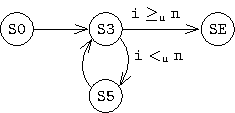
\includegraphics[scale=1.4]{chapters/figures/figMallocSpecCfg.pdf}}
\vspace{15pt}
\end{center}
\caption{\label{fig:llAllocSpecIRCFG}CFG of \SpecL{} program}
\end{subfigure}%
&
\begin{subfigure}[b]{0.5\textwidth}
\begin{center}
{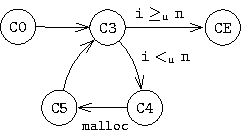
\includegraphics[scale=1.4]{chapters/figures/figMallocCCfg.pdf}}
\end{center}
\caption{\label{fig:llAllocCCFG}CFG of C program}
\end{subfigure}%
\\
\end{tabular}
\caption{\label{fig:mallocSpecCFGAndCCFG}CFG representation of Spec and C IRs shown in \cref{fig:llAllocSpecIR,fig:llAllocCIR} for the {\tt mk\_list} procedures in \cref{fig:llAllocSpec,fig:llAllocC} respectively.}
\end{figure}


\Cref{fig:llAllocSpecIRCFG,fig:llAllocCCFG} show the Control-Flow Graph (CFG) representations
of the \SpecL{} and C programs in \cref{fig:llAllocSpecIR,fig:llAllocCIR} respectively.
The CFG nodes represent PC locations of the program, and edges represent
transitions through instruction execution. For brevity, we sometimes represent
multiple program instructions with a single edge, e.g., in \cref{fig:llAllocCCFG}, the edge {\small \tt C5$\rightarrow$C3}
represents the path {\small \tt C5$\rightarrow$C6$\rightarrow$C7$\rightarrow$C8$\rightarrow$C3}. A control-flow edge is associated
with an {\em edge condition} (the condition under which that edge is taken),
a {\em transfer function} (how the program state is mutated if that edge is taken),
and a {\em UB assumption} (what condition should be true for the program
execution to be
well-defined across this edge). For example, the UB assumption associated with a division
instruction in $S$ will encode that the divisor must be non-zero.

\subsection{Product CFG}
\label{sec:productCFG}
We construct
a {\em bisimulation relation} to identify
equivalence between two programs. 
A bisimulation relation correlates
the transitions of $S$ and $C$ in lockstep, such that this
lockstep execution ensures
identical observable behavior.
An equivalence proof through bisimulation construction
can be represented using a
{\em product program} \cite{covac} and the CFG of a product program is called a {\em product-CFG}.
\Cref{fig:llAllocProductCFG} shows the CFG of the product program, also called
the product-CFG,
that encodes the lockstep execution (bisimulation relation) between the
CFGs in \cref{fig:llAllocSpecIRCFG} and \cref{fig:llAllocCCFG}. 

\begin{figure}[H]
\begin{tabular}{cc}
\begin{subfigure}[b]{1\textwidth}
\begin{center}
{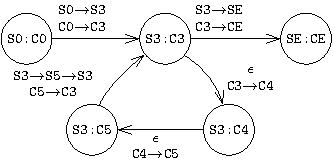
\includegraphics[scale=1.2]{chapters/figures/figMallocProductCfg.pdf}}
\end{center}
\end{subfigure}%
\end{tabular}
\caption{\label{fig:llAllocProductCFG}Product-CFG between \cref{fig:llAllocSpecIRCFG,fig:llAllocCCFG}}
\end{figure}


A node in the product-CFG is formed by pairing nodes
of $S$ and $C$ CFGs, e.g., {\tt (S3:C5)} is formed by
pairing {\tt S3} and {\tt C5}.
If the lockstep
execution is at node {\tt (S3:C5)} in the product-CFG,
then $S$'s execution is at {\tt S3} and $A$'s execution
is at {\tt C5}.
The start node {\tt (S0:C0)} of the product-CFG
correlates the start nodes of the CFGs of both programs.
Similarly, the exit node {\tt (SE:CE)}
correlates the exit nodes of the CFGs of both programs.

An edge in the product-CFG is formed by pairing a path (a sequence of edges) in $S$ with a path in $C$.
A product-CFG edge encodes the lockstep execution of correlated
transitions (or paths).
For example, the product-CFG edge {\tt (S3:C5)}$\rightarrow${\tt (S3:C3)} is formed by pairing the
{\small \tt (S3$\rightarrow$S5$\rightarrow$S3)} and {\small \tt C5$\rightarrow$C3}
in \cref{fig:llAllocSpecIRCFG,fig:llAllocCCFG},
and represents that when $S$ makes a transition {\small \tt (S3$\rightarrow$S5$\rightarrow$S3)},
then $C$ makes the transition {\small \tt C5$\rightarrow$C3}
in lockstep.
The edge {\small \tt (S3:C3)$\rightarrow$(S3:C4)}
correlates the $\epsilon$ path (no transition) in $S$ with {\small \tt C3$\rightarrow$C4} in $C$.
In general, a product-CFG edge $e$ may correlate a finite path $\rho_S$
in $S$ with a finite path $\rho_C$ in $C$,
written $e=(\rho_S,\rho_C)$.

\begin{table}[H]
\begin{center}
\caption{\label{tab:llproductInv}Node Invariants for Product-CFG in \cref{fig:llAllocProductCFG}}
\setlength{\belowcaptionskip}{-30pt}
\begin{footnotesize}
\begin{tabular}{|c|llll|}
\hline
\tt PC-Pair & \multicolumn{4}{c|} {\tt Invariants} \\
\hline
\hline
${\tt (S0:C0)}$ &
\multicolumn{4}{l|} {\Tstrut ${\tt { \circled{P}}\  n_{S}=n_{C}}$} \\
${\tt (S3:C3)}$ &
\Tstrut  ${\tt {\scriptsize \circled{I1}}\  n_{S}=n_{C}}$ & ${\tt {\scriptsize \circled{I2}}\  i_{S}=i_{C}}$ & ${\tt {\scriptsize \circled{I3}}\  i_{S} \leq_{u} n_{S}}$ & ${\tt {\scriptsize \circled{I4}}\  l_{S}\indEq{}Clist^{lnode}_{m}(l_{C})}$ \\
${\tt (S3:C4)\ (S3:C5)}$ &
\Tstrut  ${\tt {\scriptsize \circled{I5}}\  n_{S}=n_{C}}$ & ${\tt {\scriptsize \circled{I6}}\  i_{S}=i_{C}}$ & ${\tt {\scriptsize \circled{I7}}\  i_{S} <_{u} n_{S}}$ & ${\tt {\scriptsize \circled{I8}}\  l_{S}\indEq{}Clist^{lnode}_{m}(l_{C})}$ \\
${\tt (SE:CE)}$ &
\multicolumn{4}{l|} {\Tstrut  ${\tt {\circled{E}}\  ret_{S}\indEq{}Clist^{lnode}_{m}(ret_{C})}$} \\
\hline
\end{tabular}
\end{footnotesize}
\end{center}
\end{table}


At the start node {\tt (S0:C0)} of the product-CFG, the precondition $Pre$
(labeled \circled{\small P})
ensures the equality
of input arguments ${\tt n_{S}}$ and ${\tt n_{C}}$ at programs' entry.
Inductive invariants are inferred at each
product-CFG node that
relate the variables of $S$ with variables
and memory locations of $C$.
The inductive invariants
are identified by running an invariant inference
algorithm on the product-CFG. The inductive invariants
for our example are shown in \cref{tab:llproductInv}.
For example, at node {\tt (S3:C5)} in \cref{fig:llAllocProductCFG},
${\tt i}_S={\tt i}_C$ is an inductive
invariant. If the inferred invariants ensure
that the postcondition $Post$ holds at the
exit node {\tt (SE:CE)} (labeled \circled{\small E}), we have shown
equivalence of both programs.

\subsection{Recursive relations}
In \cref{tab:llproductInv}, the relation between
programs' variables at product-CFG nodes {\tt S3:C3}, {\tt S3:C4} and {\tt S3:C5}
is encoded as a \recursiveRelation{}:
``{\tt l}$_{S}\indEq{}${\tt Clist}$^{{\tt lnode}}_{m}$({\tt l}$_C$)'' where {\tt l}$_{S}$ and {\tt l}$_C$ represent the {\tt l} variables in the \SpecL{} and
C programs respectively, {\tt lnode} represents the C {\tt struct} type that contains
the {\tt value} and {\tt next} fields, and
$m$ represents a byte-addressable array representing
the current memory state of
the C program.
$l_1\indEq{}l_2$ is read {\em $l_1$ is recursively equal to
$l_2$}, i.e., $l_1$ and $l_2$ are isomorphic and
have equal
values\footnote{$l_1\indEq{}l_2$ and
$l_1=l_2$ are equivalent --- the former emphasizes
the recursive nature of the values being compared.}.
The {\em lifting constructor} {\tt Clist}$^{{\tt lnode}}_m({\tt p})$ is a
constructor that {\em lifts}
the C pointer value {\tt p} (pointing to
an object of {\tt struct lnode}) and the C
memory state $m$ to a \SpecL{} {\tt List} value.
{\tt Clist}$^{{\tt lnode}}_m({\tt p})$ is defined through its
unrolling procedure as:
\begin{small}
\begin{equation}\label{eqn:clist}
\begin{split}
U_C: \mathrm{\tt Clist}^{{\tt lnode}}_m&\mathrm{\tt (p:i32)} = \mathrm{\tt \underline{if}\ (p==0)}\ \mathrm{\tt \underline{then}\ }{\tt LNil} \\
                                                         & \mathrm{\tt \underline{else}\ {\tt LCons}(}\structPointer{p}{m}{{\tt lnode}}{val},\ {\tt Clist}_m^{\tt lnode}(\structPointer{p}{m}{{\tt lnode}}{next}))
\end{split}
\end{equation}
\end{small}
By construction, this unrolling procedure $U_C$ is
isomorphic to {\tt List}'s  unrolling procedure $U_S$ in \cref{eqn:specDeconstruct}.
``{\small $\structPointer{p}{m}{s}{f}$}'' represents the
field `{\tt f}' of the `struct {\tt s}' object pointed-to by pointer `{\tt p}'
in memory
state `$m$'.  When represented
in C-like syntax, `{\small $\structPointer{p}{m}{s}{f}$}'
is equivalent to
``{\small {\tt *((typeof s.f)*)(\&m[p+offsetof(s,f)])}}'',
%.\footnote{``{\tt offsetof(s, f)}'' represents the offset in an object of type `{\tt struct s}' where field {\tt f} lives. ``{\tt typeof s.f}'' represents the type of field {\tt f} in `{\tt struct s}'.}}\\
i.e., the expression `{\small $\structPointer{p}{m}{s}{f}$}'
returns the bytes in the memory array `$m$' starting
at address `{\small {\tt p+offsetof(s,f)}}' and interpreted as an object of
type `{\small \tt typeof s.f}'.

Note the recursive nature of the lifting value constructor {\tt Clist}: if the pointer {\tt p} of type {\tt i32}\footnote{The IR lowers integers and pointers in C to bitvectors of type {\tt i<N>}. e.g., {\tt i32} is a 32-bit bitvector type.} is zero, then this represents the empty list ({\tt LNil}); otherwise it represents the list formed by {\tt LCons}-ing
the value stored at {\tt p->value} in memory $m$ and the list formed by recursively lifting {\tt p->next} using
{\tt Clist} in memory $m$.  The recursive lifting
constructor {\tt Clist} allows us to compare C values and \SpecL{} values for equality; a
relation involving a recursive constructor is called a {\em \recursiveRelation{}}.

We later discuss in \cref{sec:searchAlgoFormal}
how a product-CFG can be constructed automatically through a counterexample-guided
search. Before that, we discuss the proof obligations that arise from a given
product-CFG. Consider the
product-CFG in \cref{fig:llAllocProductCFG}. Assuming that the precondition \circled{\small P} holds at the entry node
{\tt S0:C0} of this product-CFG, a bisimulation
check involves checking that the invariants at the other
product-CFG nodes hold too, and consequently the postcondition \circled{\small E}
holds at the exit node {\tt SE:CE}.
Recall that the precondition \circled{\small P} and the postcondition \circled{\small E}
are provided by the user, but all the other invariants are inferred automatically.

\subsection{Proof Obligations}
\label{sec:proofObligations}
We use relational Hoare triples to express these proof obligations \cite{relationalHoareLogic,hoareTriple}.
If $\phi$ denotes a predicate relating the machine states
of programs $S$ and $C$, then for a product-CFG edge $e=(\rho_S,\rho_C)$,
$\{\phi_s\} (e) \{\phi_d\}$ denotes the condition:
if the machine states $\sigma_S$ and $\sigma_C$ of programs $S$
and $C$ are related through precondition $\phi_s(\sigma_S,\sigma_C)$ and
paths $\rho_S$ and $\rho_C$ are executed in $S$
and $C$ respectively (implying the path conditions
hold), then execution terminates normally in states $\sigma_S^{'}$ (for $S$)
and $\sigma_C^{'}$ (for $C$) where
postcondition $\phi_d(\sigma_S^{'}, \sigma_C^{'})$ hold.
$\{\phi_s\} (e) \{\phi_d\}$ can also be written as
$\{\phi_s\} (\rho_S,\rho_C) \{\phi_d\}$.

For every product-CFG edge $e = (s\rightarrow d) = (\rho_S,\rho_C)$
in \cref{fig:llAllocProductCFG}, we thus
need to prove
$\{\phi_s\} (\rho_S,\rho_C) \{\phi_d\}$, where $\phi_s$ and $\phi_d$
are the node invariants
(shown
in \cref{tab:llproductInv})
at nodes $s$ and $d$ of the product-CFG respectively.
%Each set of paths (or pathset) $\xi$ is composed of multiple
%individual paths, say $\rho_1,\rho_2,...\rho_n$.
%The proof obligation, $P = (\{\phi_s\} \xi_S,\xi_C \{\phi_d\})$,
%can therefore be broken down into a sequence of
%smaller proof obligations of the form,
%$P_{ij}=(\{\phi_s\} \rho^i_S,\rho^j_C \{\phi_d\})$, where $\rho^i_S$
%and $\rho^j_C$ represent the $i$th and $j$th paths in
%pathsets $\xi_S$ and $\xi_C$ respsectively. If pathsets
%$\xi_S$ and
%$\xi_C$ contain
%$n_S$ and $n_C$ individual paths respectively, then we
%create $n_S*n_C$ smaller proof obligations $P_{ij}$ (cartesian product)
%during the discharge of $P$.
%$P$ holds iff all $P_{ij}$s hold; a counterexample that
%falsifies any $P_{ij}$ would also falsify $P$. As we will
%see later, this
%breaking down of $P$
The weakest-precondition transformer
is used to translate a Hoare triple $\{\phi_s\} (\rho_S,\rho_C) \{\phi_d\}$
to the following first-order logic formula:
\begin{equation}\label{eqn:firstOrderFormula}
(\phi_s \land pathcond_{\rho_S} \land pathcond_{\rho_C} \land ubfree_{\rho_S}) \Rightarrow {\tt WP}_{{\rho_S,\rho_C}}(\phi_d)
\end{equation}
Here, $pathcond_{\rho_X}$ represents the condition that
path $\rho_X$ is taken in program $X$.
$ubfree_{\rho_S}$ represents the condition that
the execution of program $S$ along path $\rho_S$ is
free of undefined behavior.
${\tt WP}_{{\rho_S,\rho_C}}(\phi_d)$ represents the weakest-precondition
of the predicate $\phi_d$ across the product-CFG edge $e = (\rho_S,\rho_C)$.
We will use ``{\tt LHS}'' and ``{\tt RHS}'' to
refer to the left and right hand sides of the
implication operator ``$\Rightarrow$'' in \cref{eqn:firstOrderFormula}.

\subsection{Proof Discharge Algorithm and Its Soundness}
\label{sec:proofDischarge}
We call an algorithm that evaluates the
truth value of a proof obligation, a {\em proof discharge algorithm}.
A proof discharge algorithm is {\em precise} if for all
proof obligations, the
truth value evaluated by the algorithm is identical to the
proof obligation's
{\em actual} truth value.
A proof discharge algorithm is {\em sound} if:
(a) Whenever it evaluates a proof obligation to true, the
actual truth value of that proof obligation is also true;
(b) Whenever it generates a counterexample, that counterexample
must falsify the proof obligation.
% \begin{itemize}
% \item Whenever it evaluates a proof obligation to true, the
% actual truth value of that proof obligation is also true.
% \item Whenever it generates a counterexample, that counterexample
% must falsify the proof obligation.
% \end{itemize}
However, it is possible for a sound proof discharge
algorithm to return false (without a counterexample)
when the proof obligation was actually true.

For
the proof obligations generated by our equivalence
procedure,
it is always safe for a proof discharge algorithm to
return false (without a counterexample).
If a proof
discharge algorithm conservatively
evaluates a proof obligation to false (when it
was actually true), it may
prevent the overall equivalence proof from completing successfully;
however, importantly, the overall equivalence procedure remains sound.

Resolving the truth value of a proof obligation that contains
a \recursiveRelation{} such as ${\tt l_{S}\indEq{}Clist^{{\tt lnode}}_{m}(l_{C})}$ is unclear.
Fortunately, the shapes of the proof obligations generated
by our equivalence checking algorithm are restricted, which
makes it possible to soundly resolve these proof obligations.

Our equivalence
checking algorithm ensures that, for an invariant
$\phi_s=({\tt \phi^{1}_s \land \phi^{2}_s \land ... \land \phi^{k}_s})$,
at any node $s$
of a product-CFG,
if a \recursiveRelation{} appears in $\phi_s$, it
must be one of $\phi^{1}_s$, $\phi^{2}_s$, ..., or $\phi^{k}_s$. We call
this the {\em conjunctive \recursiveRelation{}} property of an invariant $\phi_s$.

A proof obligation
$\{\phi_s\}(e)\{\phi_d\}$, where $e=(\rho_S,\rho_C)$,
gets lowered using
${\tt WP}_{e}(\phi_d)$ (as shown in \cref{eqn:firstOrderFormula}) to a first-order logic formula of the following form:
\begin{equation}\label{eqn:proofObligationShape}
({\tt \eta^{l}_1 \land \eta^{l}_2 \land ... \land \eta^{l}_m}) \Rightarrow ({\tt \eta^{r}_1 \land \eta^{r}_2 \land ... \land \eta^{r}_n})
\end{equation}
In
this formula,
the {\tt LHS} and {\tt RHS} are
written as conjunctions of $\eta^{l}_i$ and $\eta^{r}_j$ respectively (for $1\leq i\leq m$, $1\leq j\leq n$).
Each $\eta^{r}_j$ relation is obtained from
${\tt WP}_{e}(\phi^{j}_d)$, where $\phi_d=({\tt \phi^{1}_d \land \phi^{2}_d \land ... \land \phi^{n}_d})$.
Thus, due to the conjunctive \recursiveRelation{} property of $\phi_s$ and $\phi_d$, any
\recursiveRelation{} in \cref{eqn:proofObligationShape} must appear as
one of $\eta^{l}_i$ or $\eta^{r}_j$.

To simplify proof obligation discharge,
we break a first-order logic proof obligation $P$ of the form in \cref{eqn:proofObligationShape}
into multiple smaller proof obligations
of the form
$P_j:({\tt LHS}\Rightarrow{\tt \eta^{r}_j})$, for $j=1..n$. Each proof obligation
$P_j$ is then discharged separately.  We call this conversion from
a bigger query to multiple smaller queries, {\em RHS-breaking}.

%We say that two relations $\eta_1$ and $\eta_2$ {\em interfere}, written
%$\eta_1 \interfere{} \eta_2$,
%iff the intersection
%of the sets of free variables mentioned in $\eta_1$ and $\eta_2$
%is non-empty.  For example, $a\indEq{}b$ and $c\indEq{}d$
%do not interfere, but $a\indEq{}b$ and $c\indEq{}{\tt LCons}(0,b)$ interfere.
%
%In a proof obligation of the form in \cref{eqn:proofObligationShape},
%two relations $\eta_1$ and $\eta_2$ {\em transitively interfere} iff
%there exists a relation $\eta_3$ in the proof
%obligation such that $\eta_1\interfere{}\eta_3$ and $\eta_3\interfere{}\eta_2$.
%This notion of transitive interference can be lifted
%to Hoare triples: in a proof obligation $\{\phi_s\}(e)\{\phi_d\}$,
%where $\phi_{s}=\phi^{1}_s\land...\phi^{k}_{s}$ and $\phi_{d}=\phi^{1}_d\land...\phi^{n}_{d}$,
%an {\tt LHS} conjunctive clause $\phi^{i}_s$ transitively
%interferes with an {\tt RHS} conjunctive clause $\phi^{j}_d$ iff
%$\phi^{i}_s$
%transitively interferes with ${\tt WP}_{e}(\phi^{j}_d)$ in
%the lowered first-order logic formula.

%We provide a sound (but imprecise) proof discharge
%algorithm that converts
%a proof obligation generated by our equivalence
%checker into a series of SMT queries.
%Our
%algorithm begins
%by categorizing a proof obligation
%into three categories, and each
%category is discussed separately
%in subsequent sections.  These categories are created
%based on an iterative unrolling and unification
%procedure, which we describe next.
%We use an unroll parameter $k$ for
%our categorization.

\subsection{Iterative Unification and Unrolling}
\label{sec:unifyAndUnroll}

We begin with some definitions.
An expression $e$ whose top-level constructor
is a lifting constructor, e.g., $e={\tt Clist^{{\tt lnode}}_m({\tt l}_C)}$,
is called a {\em lifted expression}.
An expression $e$ of the form {\tt v.a$_1$.a$_2$...a$_n$} i.e. a variable
with {\em zero} or more {\em product deconstruction} operators applied on it, is called a {\em pseudo-variable}.
An expression $e$ in which (1) all product deconstructors (e.g. {\tt `.tail'}) appear as part
of a {\em pseudo-variable} and (2) each {\em sum-is} operator (e.g. {\tt `is LCons'})
operate on a {\em pseudo-variable}, is called a {\em canonical expression}.

Consider the expression tree of a canonical expression $e$ of ADT $T$,
formed using the ADT value constructors and the `\underline{if}-\underline{then}-\underline{else}'
sum-deconstruction operator.
% Consider an expression tree $e$ of ADT $T$\footnote{XXX:can contain value constructors of other ADT types as well}
% formed using the value constructors
% of $T$ and the `\underline{if}-\underline{then}-\underline{else}'
% sum-deconstruction operator.
The leaves of $e$ (also called atoms of $e$) are
the pseudo-variables (of scalar or ADT type),
the scalar expressions (of {\tt unit}, {\tt bool}, or {\tt i<N>} types),
and lifted expressions.

The
{\em expression path} to a node $v$ in $e$'s tree
is the path from the root of $e$
to that node $v$. The {\em expression path condition} represents
the conjunction of all the \underline{if} conditions (if
the \underline{then} branch is taken on the expression path), or their
negation (if the \underline{else} branch is taken on the
expression path) seen on the expression path.  For example,
in expression {\tt \underline{if} (c) \underline{then} a \underline{else} b},
the expression path condition of {\tt c} is {\tt true}, of {\tt a} is {\tt c},
and of {\tt b} is $\neg{\tt c}$.

When we attempt to unify two expressions, we unify the
structures created by the value constructors and the `\underline{if}-\underline{then}-\underline{else}'
operator of their canonical forms.
% When we attempt to unify two expressions, we unify the
% structures created by the value constructors and
% the \underline{if}-\underline{then}-\underline{else}
% operator of a \SpecL{} ADT.
The unification procedure either fails to unify, or it
returns tuples $(p_1,p_2,a_1,e_2)$ where atom $a_1$
at expression path condition $p_1$ in one expression is correlated with
expression $e_2$ at expression path condition $p_2$ in the other expression.

For two non-atomic expressions $e_1$
and $e_2$ to unify successfully, it must be true that
either the top-level
node in both $e_1$ and $e_2$ have the same
value constructor (in which case a unification is attempted
for each of the children of the top-level constructor),
{\em or} the top-level node in one of $e_1$ or $e_2$
is \underline{if}-\underline{then}-\underline{else.} If
the top-level node of $e_1$ is ``\underline{if} (c) \underline{then} $e^{\tt then}_1$ \underline{else} $e^{\tt else}_1$,
we attempt to unify both $e^{\tt then}_1$ and $e^{\tt else}_1$ with $e_2$ and
return success iff any of these attempts succeed (similarly for $e_2$).
Whenever we descend down an \underline{if}-\underline{then}-\underline{else} operator,
we conjunct the corresponding \underline{if} condition (for $e_1^{\tt then}$) or
its negation (for $e_1^{\tt else}$) to the respective
expression path condition. If one of
$e_1$ and $e_2$ (say $e_2$) is atomic, unification always succeeds and
returns $(p_2,p_1,e_2,e_1)$.

With each atom of an ADT type, we associate a corresponding unrolling procedure.
For example, the unrolling procedure for a \SpecL{} variable of {\tt List}
type is $U_S$ (\cref{eqn:specDeconstruct}),
whereas the unrolling procedure for a lifted expression
of type {\tt List} is $U_C$ (\cref{eqn:clist}).

Given two expressions $e_a$ and $e_b$
of an ADT $T$ at expression path conditions $p_a$ and $p_b$
respectively, an {\em iterative
unrolling and unification procedure} $\Theta(e_a,e_b,p_a,p_b)$ is used
to identify a set of correlation tuples between the
atoms in the two expressions.
This
iterative procedure
proceeds by attempting
to unify $e_a$ and $e_b$. If this unification
fails, we return a unification failure
for the original expressions $e_a$ and $e_b$. Else, we obtain
correlation between atoms and
expressions (with their expression path conditions). If the unification
correlates an atom $a_1$ at expression path condition $p_1$
with another atom $a_2$ at expression path condition $p_2$, we add $(p_1,a_1,p_2,a_2)$
to the final output.  If the unification correlates
an atom $a_1$ at expression
path condition $p_1$ to a non-atomic expression $e_2$ at
expression path condition $p_2$,
we unroll $a_1$ once using its unrolling procedure to
obtain expression $e_1$. The unification algorithm
then proceeds by unifying $e_1$ and $e_2$ through
a recursive call to $\Theta(e_1,e_2,p_a\land{}p_1,p_b\land{}p_2)$.

The maximum number of unrollings performed by
$\Theta(e_a,e_b,p_a,p_b)$ (before converging)
is upper bounded by the sum of number of $T$ value
constructors in $e_a$ and $e_b$.

If a proof obligation involves a \recursiveRelation{}
$e_a\sim{}e_b$, we unify $e_a$ and $e_b$
through a call to $\Theta(e_a, e_b, {\tt true}, {\tt true})$.
For example,
the unification of ``{\tt \underline{if} (c$_1$) \underline{then} LNil \underline{else} LCons(0, l$_S$)}'' and
``{\tt \underline{if} (c$_2$) \underline{then} LNil \underline{else} LCons(0, {\tt Clist$^{{\tt lnode}}_m({\tt l}_C)$})}''
yields the correlation
tuples: {\tt (c$_1$,(),c$_2$,())}, {\tt ($\neg$c$_1$,0,$\neg$c$_2$,0)} and {\tt ($\neg$c$_1$,l$_S$,$\neg$c$_2$,$Clist^{{\tt lnode}}_m({\tt l}_C)$)}.

If the set of $n$ tuples obtained
after a successful unification
of $e_a\sim{}e_b$
are $(p^i_1, a^i_1, p^i_2, a^i_2)$ (for $i=1\ldots{}n$), then
$e_a\indEq{}e_b \Leftrightarrow{} \bigwedge\limits_{i=1}^n((p^i_1=p^i_2) \land ((p^i_1\land{}p^i_2)\rightarrow{}(a^i_1=a^i_2)))$\footnote{If $a^i_1$ and $a^i_2$ are recursive data structures, then we replace $a^i_1=a^i_2$ with $a^i_1\indEq{}a^i_2$.}.
We call
$\bigwedge\limits_{i=1}^n((p^i_1=p^i_2) \land ((p^i_1\land{}p^i_2)\rightarrow{}(a^i_1=a^i_2)))$
the {\em decomposition}
of $e_a\indEq{}e_b$.
Each conjunctive clause of one of the forms $(p^i_1=p^i_2)$ and $((p^i_1\land{}p^i_2)\rightarrow{}(a^i_1=a^i_2))$ in
this decomposition is called a {\em decomposition clause}.
A decomposition clause may relate only atomic values, i.e.,
in the decomposed form, all recursive relations
relate only ADT variables and/or lifted expressions.
The decomposition for a failed unification is defined as {\tt false}.
We {\em decompose}
a \recursiveRelation{} by replacing it with its
decomposition.
We {\em decompose} a proof obligation $P$ by
decomposing all recursive relations in $P$.
%Further, we 

\subsection{$k$-unrolling with respect to an unrolling procedure}
We can {\em unroll an expression $e$ with respect to an unrolling
procedure $U$}
by substituting all occurrences
of the constructor ({\tt LHS} in $U$) by its
unrolled version ({\tt RHS} in $U$) and decomposing it.
For example, an unrolling
of ${\tt LHS}\Rightarrow{}{\tt l_S\indEq{}Clist^{{\tt lnode}}_{m}(0)}$
with respect to $U_C$ (\cref{eqn:clist})
yields
$P: {\tt LHS}\Rightarrow{}{\tt l_S\indEq{}LNil}$.
Unrolling $P$ with respect to $U_S$ (\cref{eqn:specDeconstruct})
yields
${\tt LHS}\Rightarrow{}{\tt l_S\ \ is\ \ LNil}$.

A $k$-unrolling of an expression $e$ w.r.t. unrolling procedure $U$
is obtained by unrolling a $(k-1)$ unrolling of $e$ w.r.t. $U$.
We say an expression $e$ is $k$-unrolled (without specifying
the unrolling procedure $U$), we imply that
$e$ is $k$-unrolled with respect to the unrolling procedures of
{\em all} the lifting constructors appearing in $e$.

For a first-order
logic proof obligation
$P: {\tt LHS}\Rightarrow{\tt RHS}$, we identify
a $k$-unrolling of $P$ (for a fixed unrolling parameter $k$).
After unrolling,
we eliminate those decomposition clauses
$(p^i_1\land{}p^i_2)\rightarrow{}(a^i_1=a^i_2)$ whose
path condition $(p^i_1\land{}p^i_2)$ evaluates to false
under the non-recursive conjunctive clauses in the {\tt LHS}. We categorize the proof obligation based
on this $k$-unrolled form of $P$.

\subsection{Category 1: The $k$-unrolled form of $P$
contains no recursive relations}
\label{sec:cat1}
In \cref{fig:llAllocProductCFG}, consider a proof obligation generated
across the product-CFG edge ${\tt (S0:C0) \rightarrow (S3:C3)}$
while checking if the ${\small \circled{I4}}$ invariant, $l_{S}\indEq{}Clist^{{\tt lnode}}_{m}(l_{C})$,
holds at {\tt (S3:C3)}:
$\{\phi_{{\tt S0:C0}}\} ({\tt S0\rightarrow S3}, {\tt C0\rightarrow C3}) \{l_{S}\indEq{}Clist^{{\tt lnode}}_{m}(l_{C})\}$.
The precondition $\phi_{{\tt S0:C0}}=(n_S=n_C)$ does not contain
a \recursiveRelation{}.
When lowered to first-order logic through {\tt WP$_{{\tt S0\rightarrow S3},{\tt C0\rightarrow C3}}$}, this translates to
``$(n_S=n_C)\Rightarrow({\tt LNil}\indEq{}{\tt Clist^{{\tt lnode}}_{m}(0)})$''.
Here, {\tt LNil} is obtained for {\tt l$_{S}$} and {\tt 0} (or NULL) is
obtained for {\tt l$_C$}.
The one-unrolled form of this proof obligation yields
$(n_S=n_C)\Rightarrow{}{\tt LNil}\indEq{}{\tt LNil}$ which trivially resolves to true.

Consider another example of a proof obligation,
$\{\phi_{{\tt S0:C0}}\} ({\tt S0\rightarrow S3\rightarrow S5\rightarrow S3}, \\{\tt C0\rightarrow C3}) \{l_{S}\indEq{}Clist^{{\tt lnode}}_{m}(l_{C})\}$.
Notice, we have changed the path in $S$ to ${\tt S0\rightarrow S3\rightarrow S5\rightarrow S3}$ here.
In this case, the corresponding first-order logic condition evaluates
to: ``$(n_S=n_C)\Rightarrow({\tt LCons(0, LNil)}\indEq{}{\tt Clist^{{\tt lnode}}_{m}(0)})$''.
The one-unrolled form of this proof obligation converts
${\tt Clist^{{\tt lnode}}_{m}(0)}$ to {\tt LNil}, and
decomposes {\tt RHS} into {\tt false} (due to failed unification).
The proof obligation is further discharged using an SMT solver
which provides a counterexample (model) that evaluates the
formula to false. For example, the counterexample {\tt \{ n$_S$ $\mapsto$ 42, n$_C$ $\mapsto$ 42 \} }
evaluates this formula to false.
% because
% this fails to unify (during decomposition), it evaluates to false.
% When a
% proof obligation evaluates to false, the SMT solver
% provides a counterexample (model) that evaluates the condition
% to false.  For example, the counterexample {\tt n$_S$=n$_C$=42}
% evaluates this condition to false.
These counterexamples
assist in faster convergence
of our invariant inference and correlation search procedures (as we will discuss later).

Thus, we unify the structure and
values of the \SpecL{} objects on both sides of
the $\sim$ operator (after $k$ unrollings), and discharge the resulting
proof obligations (that relate bitvector and array values) using an SMT solver.
A more detailed workings of the procedure for discharging SMT proof obligations and handling counter-examples is given
in \cref{sec:smtdischarge}.
Assuming a capable enough SMT solver,
all proof obligations in Category 1 can be discharged precisely, i.e.,
we can always decide whether $P$ evaluates to true or false. If it
evaluates to false, we also obtain a counterexample.

\begin{figure}
\begin{tabular}{cc}
\begin{subfigure}[b]{0.45\textwidth}
\begin{center}
\begin{allLangEnvFoot}
~{\scriptsize \textcolor{mygray}{   }}~   
~{\scriptsize \textcolor{mygray}{S0:}}~ i32 sum_list (List l) {
~{\scriptsize \textcolor{mygray}{S1:}}~   i32 sum $\coloneqq$ ${\tt 0_{i32}}$;
~{\scriptsize \textcolor{mygray}{S2:}}~   while $\mathrm{\tt\neg (l\ is\ LNil)}$:
~{\scriptsize \textcolor{mygray}{S3:}}~     // (l is LCons);
~{\scriptsize \textcolor{mygray}{S4:}}~     sum $\coloneqq$ sum + ${\tt l.val}$;
~{\scriptsize \textcolor{mygray}{S5:}}~     l   $\coloneqq$ l.next;
~{\scriptsize \textcolor{mygray}{S6:}}~   return sum;
~{\scriptsize \textcolor{mygray}{SE:}}~ }
\end{allLangEnvFoot}
\end{center}
\caption{\label{fig:llTraverseSpec}(Abstracted) Spec IR}
\end{subfigure}%
&
\begin{subfigure}[b]{0.55\textwidth}
\begin{center}
\begin{allLangEnvFoot}
~{\scriptsize \textcolor{mygray}{\ \ \ }}~ unsigned sum_list (lnode* l);
~{\scriptsize \textcolor{mygray}{C0:}}~ i32 sum_list (i32 l) {
~{\scriptsize \textcolor{mygray}{C1:}}~   i32 sum $\coloneqq$ ${\tt 0_{i32}}$;
~{\scriptsize \textcolor{mygray}{C2:}}~   while ${\tt l \neq 0_{i32}}$:
~{\scriptsize \textcolor{mygray}{C3:}}~     sum $\coloneqq$ sum + $\structPointer{\tt l}{m}{\tt lnode}{val}$;
~{\scriptsize \textcolor{mygray}{C4:}}~     l   $\coloneqq$ $\structPointer{\tt l}{m}{\tt lnode}{next}$;
~{\scriptsize \textcolor{mygray}{C5:}}~   return sum;
~{\scriptsize \textcolor{mygray}{CE:}}~ }
\end{allLangEnvFoot}
\end{center}
\caption{\label{fig:llTraverseC}(Abstracted) C IR}
\end{subfigure}%
\\
\begin{subfigure}[b]{0.45\textwidth}
\begin{center}
{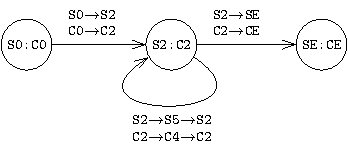
\includegraphics[scale=1.1]{chapters/figures/figSumListProductCfg.pdf}}
\end{center}
\caption{\label{fig:llTraverseProduct}Product-CFG}
\end{subfigure}%
&
\begin{subfigure}[b]{0.55\textwidth}
\begin{center}
\begin{footnotesize}
\begin{tabular}{|c|l|}
\hline
\tt PC-Pair & \multicolumn{1}{c|} {\tt Invariants} \\
\hline
\hline
${\tt (S0:C0)}$ &
\Tstrut ${\tt {\circled{P}}\  l_{S}\indEq{}Clist^{lnode}_{m}(l_{C})}$ \\
\multirow{2}{*}{${\tt (S2:C2)}$} &
\Tstrut \Bstrut ${\tt {\scriptsize \circled{I1}}\  l_{S}\indEq{}Clist^{lnode}_{m}(l_{C})}$ \\ & ${\tt {\scriptsize \circled{I2}}\  sum_{S}=sum_{C}}$ \\
${\tt (SE:CE)}$ &
\Tstrut \Bstrut ${\tt {\circled{E}}\  ret_{S}=ret_{C}}$ \\
\hline
\end{tabular}
\end{footnotesize}
\vspace{13px}
\end{center}
\caption{\label{fig:llTraverseProductInv}Node Invariants of the Product-CFG}
\end{subfigure}%
\\
\end{tabular}
\caption{\label{fig:llTraverseSpecAndC}Spec and C programs for traversing a linked list. \Cref{fig:llTraverseProduct} shows the Product-CFG between the IRs in \cref{fig:llTraverseSpec,fig:llTraverseC}. The inductive invariants of the Product-CFG are given in \cref{fig:llTraverseProductInv}.}
\end{figure}


\subsection{Category 2: The $k$-unrolled form of $P$
contains a \recursiveRelation{} in the LHS but not in the RHS}
\label{sec:cat2}

Consider the pair of programs in \cref{fig:llTraverseSpec,fig:llTraverseC}
that traverse a list to compute the sum of all elements.
The corresponding product-CFG and its node
invariants that ensure observable
equivalence are shown in \cref{fig:llTraverseProduct,fig:llTraverseProductInv}.

Consider
the proof obligation $\{\phi_{{\tt S2:C2}}\} ({\tt S2\rightarrow S4\rightarrow S2}, {\tt C2\rightarrow C4\rightarrow C2}) \{sum_{S} = sum_{C}\}$, where
the node invariant $\phi_{{\tt S2:C2}}$ contains
the \recursiveRelation{} $l_{S}\indEq{}Clist^{{\tt lnode}}_{m}(l_{C})$.
The corresponding (simplified) first-order logic condition for this
proof obligation is:
($l_{S}\indEq{}Clist^{{\tt lnode}}_{m}(l_{C}) \land {\tt sum}_S={\tt sum}_C \land \neg({\tt l_S}\ is\ {\tt Nil})) \Rightarrow (({\tt sum}_S + l_S.val) = (sum_C + \structPointer{l}{m}{{\tt lnode}}{val}))$.
The problem here is that we do not know of an efficient
SMT encoding for the \recursiveRelation{} ($l_{S}\indEq{}Clist^{{\tt lnode}}_{m}(l_{C})$)
and we fail to construct a non-recursive proof obligation even
after $k$ unrollings of this \recursiveRelation{}.
Ignoring this \recursiveRelation{} will incorrectly (although soundly) evaluate
the proof obligation to false; however, for a successful equivalence
proof, we need
the proof discharge algorithm to evaluate it to true. Let's call this
requirement \circled{\small R1}.

Now, consider the proof obligation formed by correlating two iterations
of the loop in program $S$ with one iteration of the loop in program $C$,
$\{\phi_{{\tt S2:C2}}\} ({\tt S2\rightarrow S4\rightarrow S2\rightarrow S4\rightarrow S2}, {\tt C2\rightarrow C4\rightarrow C2}) \{sum_{S} = sum_{C}\}$.
The equivalent
first-order logic condition is:
($l_{S}\indEq{}Clist^{{\tt lnode}}_{m}(l_{C}) \land {\tt sum}_S={\tt sum}_C \land \neg({\tt l_S}\ is\ {\tt Nil}) \land \neg({\tt l_S.tail}\ is\ {\tt Nil})) \Rightarrow (({\tt sum}_S + l_S.val + l_S.tail.val) = (sum_C + \structPointer{l}{m}{{\tt lnode}}{val}))$.  After one unrolling
of $l_{S}\indEq{}Clist^{{\tt lnode}}_{m}(l_{C})$,
this proof obligation evaluates to false.
Whenever a proof
obligation evaluates to false, we
expect an ideal proof discharge algorithm to generate a
counterexample that falsifies the proof condition.
Let's call this
requirement \circled{\small R2}.
Recall that such counterexamples help in faster
convergence of our invariant inference and correlation algorithms.

To tackle requirements \circled{\small R1} and \circled{\small R2},
our proof discharge algorithm converts the
original proof obligation
$P: \{\phi_s\} (e) \{\phi_d\}$
into two approximated proof obligations:
$(P_{{\tt pre-o}}: \{\phi^{o_{d_1}}_s\} (e) \{\phi_d\})$
and
$(P_{{\tt pre-u}}: \{\phi^{u_{d_2}}_s\} (e) \{\phi_d\})$. Here
$\phi^{o_{d_1}}_s$ and
$\phi^{u_{d_2}}_s$ represent the over- and under-approximated
versions of precondition $\phi_s$ respectively, and $d_1$ and $d_2$ represent
{\em depth} parameters that indicate the degree of over- and
under-approximation.
To explain
our over- and under-approximation scheme, we
first need to
introduce the notion of the {\em depth of an ADT value}.

\subsubsection{Depth of an ADT value}
To define the depth of an ADT value,
we view the ADT as a context-free grammar:
\begin{itemize}
\item The set of terminals
consist of (a) scalar values, e.g., {\tt 42} for the {\tt i32} type, and
(b) the ADT value constructors (e.g., {\tt LNil}, {\tt LCons}).
\item The set of non-terminals are all the scalar type identifiers ({\tt i32}, {\tt bool}, {\tt unit})
and all the ADT type identifiers (e.g., {\tt List}, {\tt Tree}, {\tt Matrix2D}).
\item Productions of this context-free grammar specify the values that may be constructed for each type identifier: (a) For each basic type (e.g. {\tt i32}), we add productions from its type identifier to all values of that type, e.g., {\tt i32 $\rightarrow$ 0|1|2|...|($2^{32}-1$)};
(b) For an ADT, each constructor represents a separate production rule,
e.g., ADT {\tt List} has two productions: {\tt List} $\rightarrow$ {\tt LNil} | {\tt LCons} {\tt i32} {\tt List}.
% \begin{itemize}
% \item For each basic type (e.g. {\tt i32}), we add productions from its type identifier to all values of that type, e.g., {\tt i32 $\rightarrow$ 0|1|2|...|($2^{32}-1$)},
% \item For an ADT, each constructor represents a separate production rule,
% e.g. ADT {\tt List} has two productions: {\tt List} $\rightarrow$ {\tt LNil} | {\tt LCons} {\tt i32} {\tt List}.
% \end{itemize}
\item The start non-terminal is the top-level ADT identifier (e.g., {\tt List}).
\end{itemize}
In this context-free grammar interpretation of an ADT, a value of this ADT type
can be viewed as a {\em parse tree} (also called a derivation tree) of the
grammar.
The {\em depth} of a node in this parse tree is the number
of ADT identifiers (but not scalar type identifiers) in the
path from the root node to the node representing that terminal value (both inclusive).
\Cref{fig:parseTrees} shows examples of values of the {\tt List}, {\tt Tree},
and {\tt Matrix2D} ADTs, and the depth values of the parse tree nodes.
The {\em maximum depth of an ADT value} is the maximum depth of any node
in the parse tree of that value.

\begin{figure}[t]
\begin{tabular}{ccc}
\begin{subfigure}[b]{0.32\textwidth}
\begin{center}
{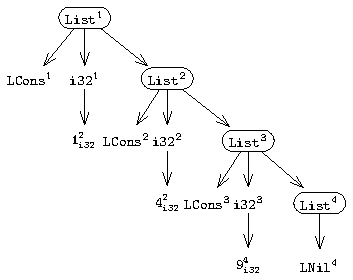
\includegraphics[scale=0.8]{chapters/figures/figParseTreeList3.pdf}}
\end{center}
\caption{\label{fig:listParseTree}{\small\tt List = LNil | \newline LCons(i32, List)}}
\end{subfigure}%
&
\begin{subfigure}[b]{0.22\textwidth}
\begin{center}
{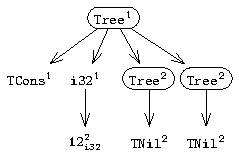
\includegraphics[scale=0.78]{chapters/figures/figParseTreeTree2.pdf}}
\vspace{10px}
\end{center}
\caption{\label{fig:treeParseTree}{\footnotesize\tt Tree = TNil | \newline TCons(i32, Tree, Tree)}}
\end{subfigure}%
&
\begin{subfigure}[b]{0.4\textwidth}
\begin{center}
{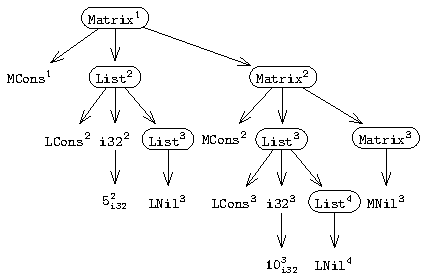
\includegraphics[scale=0.78]{chapters/figures/figParseTreeMatrix2.pdf}}
\end{center}
\caption{\label{fig:matrixParseTree}{\tt Matrix = MNil | \newline MCons(List, Matrix)}}
\end{subfigure}%
\\
\end{tabular}
\vspace{-12px}
\caption{\label{fig:parseTrees}Parse Trees with Depths (shown as superscript) for {\tt List}, {\tt Tree}, and {\tt Matrix}}
\end{figure}

\vspace{-6px}
\subsubsection{Overapproximation and Underapproximation}
To overapproximate (underapproximate)
a precondition $\phi$, each
conjunctive \recursiveRelation{} in $\phi$ is overapproximated (underapproximated)
individually.

The $d$-depth overapproximated
version of a \recursiveRelation{}
$l_1\indEq{}l_2$ is written as $l_1\indEqDepth{d} l_2$, where
$\indEqDepth{d}$ represents the condition that the two ADT values
$l_1$ and $l_2$ are {\em recursively equal up to depth $d$}. i.e., all
{\em terminals} at depth $\leq d$ in the parse trees of both values
are identical; however, terminals at depths $>d$ can have
different values.
$l_1\indEqDepth{d}l_2$ (for finite $d$) is a weaker
condition than $l_1\indEq{}l_2$ (overapproximation);
$l_1\indEq{}l_2$
is equivalent to
$l_1\indEqDepth{\infty}l_2$.

The $d$-depth underapproximated
version of a \recursiveRelation{}
$l_1\indEq{}l_2$ is written
as $l_1\indEqUapprox{d}l_2$, where $\indEqUapprox{d}$ represents
the condition that the two ADT values $l_1$ and $l_2$ are
{\em recursively equal and bounded to depth $d$}, i.e.,
$l_1$, $l_2$ have a maximum
depth $\leq d$ {\em and} they are recursively equal up to depth $d$.
Thus, $l_1\indEqUapprox{d}l_2$ is equivalent
to
$((l_1\indEqDepth{d} l_2)\land\depthBound{d}{l_1}\land\depthBound{d}{l_2})$,
where $\depthBound{d}{l}$ represents the condition that the maximum
depth of $l$ is $d$.
$l_1\indEqUapprox{d}l_2$ (for finite $d$)
is a stronger condition than $l_1\indEq{}l_2$ (underapproximation)
as it ensures both equality and max-depth of both values.
$l_1\indEq{}l_2$
is equivalent to
$l_1\indEqUapprox{\infty}l_2$.

\subsubsection{SMT encoding of overapproximate and underapproximate proof obligations}
\label{sec:ouapprox}
Unlike the original \recursiveRelation{} $l_1\indEq{}l_2$,
$l_1\indEqDepth{d}l_2$ and
$l_1\indEqUapprox{d}l_2$ can be encoded using SMT through {\em unrolling
till depth $d$}:
\begin{itemize}
\item $l_1\indEqDepth{d}l_2$ is equivalent to the condition
that the parse tree structures
of the two values $l_1$ and $l_2$ (after $d$-unrolling)
are isomorphic till depth $d$ {\em and} the
corresponding values in both ($d$-depth)
isomorphic structures
are also equal.
$l_1\indEqDepth{d}l_2$ can be identified through d-unrolling followed by removal of all conjunctive clauses containing \recursiveRelations{}.

For example, for {\tt List} values $l_1$
and $l_2$, the
condition $l_1\indEqDepth{1}{\tt Clist}^{{\tt lnode}}_{m}({\tt p})$
can be one-unrolled to:
\begin{small}
\begin{center}
\underline{if} $l_1$ {\em is} {\tt LNil} \underline{then} {\tt LNil} \underline{else} {\tt LCons($l_1$.val,$l_1$.tail)}\\
$\indEqDepth{1}$\\
$\mathrm{\tt \underline{if}\ (p==0)\ \underline{then}\ }{\tt LNil}\mathrm{\tt \ \underline{else}\ {\tt LCons}(}\structPointer{p}{m}{{\tt lnode}}{val},\ {\tt Clist}^{{\tt lnode}}_m(\structPointer{p}{m}{{\tt lnode}}{next}))$.
\end{center}
\end{small}
The decomposition of the
condition shown above
reduces to the SMT-encodable condition:
\begin{small}
$$
((l_1\ \ is\ \ {\tt LNil}) \Leftrightarrow {\tt (p == 0)}) \land (\neg(l_1\ \ is\ \ {\tt LNil})\Rightarrow(l_1{\tt.val}=\structPointer{p}{m}{{\tt lnode}}{val}))
$$
\end{small}

%This condition relates the structure (by equating the \underline{if}-\underline{then}-\underline{else} path
%conditions) and values (by equating the terminals if their respective path conditions evaluate to true) up to
%depth one. It is silent on the structure and values of the parse tree nodes at depth $>1$.

%Unrolling can be performed by recursively substituting any ADT values
%with their \underline{if}-\underline{then}-\underline{else} decomposition.
%For example, to obtain a two-unrolled version of the condition
%$l_1\indEqDepth{1}{\tt Clist}^{{\tt lnode}}_{m}({\tt l}_C)$,
%we take all the ADT values in the one-unrolled version,
%namely {\tt $l_1$.tail} and ${\tt Clist}^{{\tt lnode}}_m\mathrm{(p}\xrightarrow[]{m}_{{\tt lnode}}\mathrm{\tt next})$,
%and substitute them with their respective
%\underline{if}-\underline{then}-\underline{else} decompositions.

\item $\depthBound{d}{l}$ is equivalent to the condition
that the parse-tree nodes at depths
$>d$ are unreachable. This is achieved by unrolling a \recursiveRelation{}
till depth $d$ and then asserting the unreachability
of
\underline{if}-\underline{then}-\underline{else}
paths that reach nodes with depth $>d$ (by checking the
satisfiability of their expression path conditions).
For example, for a {\tt List} value $l$,
the condition
$\depthBound{2}{l}$ is equivalent to
$(l\ \ is\ \ {\tt LNil}) \vee (\neg(l\ \ is\ \ {\tt LNil})\land(l{\tt .tail}\ \ is\ \ {\tt LNil}))$.
Similarly,
$\depthBound{2}{{\tt Clist}^{{\tt lnode}}_{m}({\tt p})}$
is equivalent to
$({\tt p}=0) \vee (\neg({\tt p}\neq 0)\land({\tt p}\xrightarrow[]{m}_{{\tt lnode}}\mathrm{\tt next}=0))$.
\end{itemize}

\subsubsection{Proof discharge algorithm for Category 2 proof obligations}
\label{sec:cat2algo}
Thus, for a {\em Category 2} proof obligation
$P: \{\phi_s\} (e) \{\phi_d\}$, we first
submit the proof obligation
$(P_{{\tt pre-o}}: \{\phi^{o_{d_1}}_s\} (e) \{\phi_d\})$
to the SMT solver. Recall that the precondition $\phi^{o_{d_1}}_s$
is the overapproximated version
of $\phi_s$.
If the SMT solver evaluates
$P_{{\tt pre-o}}$ to true, then we return true for
the original proof obligation $P$ --- if the
Hoare triple with an overapproximate precondition
holds, then the original Hoare triple
also holds.

If the
SMT solver evaluates
$P_{{\tt pre-o}}$ to false, then we submit
the proof obligation
$(P_{{\tt pre-u}}: \{\phi^{u_{d_2}}_s\} (e) \{\phi_d\})$
to the SMT solver. Recall that the precondition $\phi^{u_{d_2}}_s$
is the underapproximated version of $\phi_s$.
If the SMT solver evaluates
$P_{{\tt pre-u}}$ to false, then we return false for
the original proof obligation $P$ --- if the
Hoare triple with an underapproximate precondition
does not hold, then the original Hoare triple
also does not hold. Further, a counterexample that
falsifies $P_{{\tt pre-u}}$ would also falsify $P$,
and is thus usable in invariant inference and correlation procedures.
% and is thus a valid counterexample for use in invariant
% inference and correlation procedures.

Finally, if the SMT solver evaluates
$P_{{\tt pre-u}}$ to true, then we have neither
proven nor disproven $P$. In this case, we
imprecisely (but soundly) return false for the
original proof obligation $P$ (without a counterexample).
Revisiting our examples,
the proof obligation $\{\phi_{{\tt S2:C2}}\} ({\tt S2\rightarrow S4\rightarrow S2}, {\tt C2\rightarrow C4\rightarrow C2}) \\ \{sum_{S} = sum_{C}\}$ is provable using a depth-1 overapproximation of the
precondition $\phi_{{\tt S2:C2}}$ --- the depth-1 overapproximation retains the
information that the first value in lists ${\tt l}_S$
and ${\tt l}_C$ are equal, and that is sufficient to prove that
the new values of $sum_{S}$ and $sum_{C}$ are also equal (given that the
old values are equal, as encoded in $\phi_{{\tt S2:C2}}$).

Similarly, the proof obligation
$\{\phi_{{\tt S2:C2}}\} ({\tt S2\rightarrow S4\rightarrow S2\rightarrow S4\rightarrow S2}, {\tt C2\rightarrow C4\rightarrow C2}) \{sum_{S} = sum_{C}\}$ evaluates to false (with a counterexample) using
a depth-2 underapproximation of the precondition $\phi_{{\tt S2:C2}}$.
In the depth-2 underapproximate version, we try to prove that
if the equal lists $l_S$ and ${\tt Clist}^{{\tt lnode}}_{m}(l_C)$
have exactly two
nodes\footnote{The underapproximation
restricts both lists to have at most
two nodes; the path condition for ${\tt S2\rightarrow S4\rightarrow S2\rightarrow S4\rightarrow S2}$ additionally
restricts $l_S$ to have at least two nodes; together, this is equivalent to the list having
exactly two nodes}, then
the sum of the values in the two nodes of $l_S$ is equal to the
value stored in the first node in {\tt l}$_C$.
This proof obligation will return a counterexample that
maps program variables to their concrete values. We show a
possible counterexample to this proof obligation below.
%
\begin{center}
\begin{footnotesize}
\begin{tabular}{cc|c}
{\tt sum$_S$ $\mapsto$ 3} & {\tt sum$_C$ $\mapsto$ 3} & \multirow{3}{*}{
$m$ $\mapsto$ $\Bigg($
\begin{tabular}{l}
{\tt 0x123} $\mapsto_{\tt lnode}$ (.value $\mapsto$ 42, .next $\mapsto$ {\tt 0x456}), \\
{\tt 0x456} $\mapsto_{\tt lnode}$ (.value $\mapsto$ 43, .next $\mapsto$ {\tt 0x000}), \\
() $\mapsto$ {\tt 77} \\
\end{tabular}
$\Bigg)$
} \\
\multicolumn{2}{l|}{{\tt l$_S$} $\mapsto$ {\tt LCons(42,LCons(43,LNil))}} \\
\multicolumn{2}{l|}{{\tt l$_C$} $\mapsto$ {\tt 0x123}} \\
\end{tabular}
\end{footnotesize}
\end{center}
% \begin{center}
% \begin{footnotesize}
% \begin{tabular}{l@{ $\mapsto$ }l|l}
% {\tt sum$_S$} & {\tt 3} &
% \multirow{4}{*}{
% $m$ $\mapsto$ $\Bigg($
% \begin{tabular}{l}
% {\tt 0x123} $\mapsto_{\tt lnode}$ (.value $\mapsto$ 42, .next $\mapsto$ {\tt 0x456}), \\
% {\tt 0x456} $\mapsto_{\tt lnode}$ (.value $\mapsto$ 43, .next $\mapsto$ {\tt 0x000}), \\
% () $\mapsto$ {\tt 77} \\
% \end{tabular}
% $\Bigg)$
% }
% \\
% {\tt sum$_C$} & {\tt 3} \\
% ${\tt l}_S$   & {\tt LCons(42,LCons(43,LNil))} \\
% ${\tt l}_C$   & {\tt 0x123} \\
% \end{tabular}
% \end{footnotesize}
% \end{center}

% \begin{center}
% \begin{tabular}{ll@{ $\mapsto$ }l}
% \{ & {\tt sum$_S$} & {\tt 3},\\
%    & {\tt sum$_C$} & {\tt 3},\\
%    & ${\tt l}_S$ & {\tt LCons(42,LCons(43,LNil))},\\
%    & ${\tt l}_C$ & {\tt 0x123},\\
%    & $m$ & $\bigg($
%            \begin{tabular}{ll}
%              & {\tt 0x123} $\mapsto_{\tt lnode}$ (.value $\mapsto$ 42, .next $\mapsto$ {\tt 0x456}),\\
%               & {\tt 0x456} $\mapsto_{\tt lnode}$ (.value $\mapsto$ 43, .next $\mapsto$ 0),\\
%               & () $\mapsto$ {\tt 77}\\
%            \end{tabular}$\bigg)$ \\
% \}\\
% \end{tabular}
% \end{center}

This counterexample maps variables to values (e.g., {\tt sum}$_C$ maps to an {\tt i32} value {\tt 3}
and {\tt l}$_S$ maps to a {\tt List} value {\tt LCons(42,LCons(43,LNil))}).
It also maps the C program's memory state $m$ to an array that
maps the regions starting at addresses {\tt 0x123} and {\tt 0x456} (regions of size
`{\tt sizeof lnode}') to memory objects of type {\tt lnode} (with the
{\tt value} and {\tt next} fields shown for each object). For all other addresses (except
the ones for which an explicit mapping is available), $m$ maps them
to the default byte-value {\tt 77} (shown
as {\tt () $\mapsto$ 77}) in this counterexample.

This counterexample satisfies the preconditions $l_S\indEqUapprox{2}{\tt Clist}^{{\tt lnode}}_{m}({\tt l}_C)$
and $sum_S=sum_C$. Further, when the
paths $({\tt S2\rightarrow S4\rightarrow S2\rightarrow S4\rightarrow S2}, {\tt C2\rightarrow C4\rightarrow C2})$
are executed starting at the machine state represented by this counterexample, the resulting
values of $sum_S$ and $sum_C$ are {\tt 3+42+43=88} and {\tt 3+42=45} respectively. Evidently, the
counterexample falsifies the proof condition because these values are not equal (as required by the postcondition).
\vspace{-6px}
\subsection{Category 3: The $k$-unrolled form of $P$ contains a \recursiveRelation{} in RHS and optionally LHS as well}
\label{sec:cat3}
In \cref{fig:llAllocProductCFG}, consider a proof obligation generated
across the product-CFG edge ${\tt (S3:C5) \rightarrow (S3:C3)}$
while checking if the {\small $\circled{I4}$} invariant, $l_{S}\indEq{}Clist^{lnode}_{m}(l_{C})$,
holds at {\tt (S3:C3)}:
$\{\phi_{{\tt S3:C5}}\} ({\tt S3\rightarrow S5\rightarrow S3}, \\ {\tt C5\rightarrow C3}) \{l_{S}\indEq{}Clist^{lnode}_{m}(l_{C})\}$.
Here, a \recursiveRelation{} is present both in the precondition $\phi_{{\tt S3:C5}}$ ({\small \circled{I8}})
and in the postcondition ({\small \circled{I4}}) and we could
not remove them even after $k$ unrollings and unification.
When lowered to first-order logic
through {\tt WP$_{{\tt S3\rightarrow S5\rightarrow S3},{\tt C5\rightarrow C3}}$}, this translates to (showing only relevant
relations):
\vspace{-5px}
\begin{small}
\begin{equation}\label{eqn:ex1cat3}
({\tt i}_S={\tt i}_C \land {\tt p}_C={\tt malloc()} \land {\tt l}_S \indEq{} {\tt Clist}_m^{{\tt lnode}}({\tt l}_C)) \Rightarrow ({\tt LCons}({\tt i}_S, {\tt l}_S) \indEq{} {\tt Clist}_{m'}^{{\tt lnode}}({\tt p}_C))
\end{equation}
\end{small}
On the {\tt RHS} of this first-order logic formula, {\tt LCons(i, l$_S$)} is compared for
equality with {\tt Clist$_{m'}^{{\tt lnode}}$(p$_C$)}; here {\tt p$_C$}
represents the address of the newly allocated {\tt lnode} object (through {\tt malloc}) and $m'$
represents the C memory state after executing the writes at lines
{\tt C5} and {\tt C6} on the path {\tt C5$\rightarrow$C3},
i.e.,
\vspace{-5px}
\begin{small}
\begin{equation}\label{eqn:memstore}
m' \equiv m[{\tt \&(p}_C\xrightarrow[]{m}_{\mathrm{\tt lnode}}{\tt value}) \leftarrow {\tt i}_C]_{\tt i32}[{\tt \&(p}_C\xrightarrow[]{m}_{\mathrm{\tt lnode}}{\tt next}) \leftarrow {\tt l}_C]_{\tt i32}
\end{equation}
\end{small}
Here, $m[{\tt a}\leftarrow{\tt v}]$ reprsents an array that is
formed by writing value {\tt v} to address {\tt a} in array $m$.
We also refer to
these memory writes that distinguish $m$ from $m'$, the {\em distinguishing writes}.

\subsubsection{Replacing \SpecL{} recursive values in the RHS with lifted C values}
\toolName{} utilizes
the $\indEq{}$ relationships in the {\tt LHS} (antecedant) of ``$\Rightarrow$''
to rewrite \cref{eqn:ex1cat3}
so that the recursive {\tt List} values in its {\tt RHS} (conclusion)
are replaced with the lifted $C$ values (lifted using
the {\tt Clist} constructor). Thus, we
rewrite \cref{eqn:ex1cat3} to:
%\begin{equation}\label{eqn:clistsEqualUnder}
%({\tt l}_S \indEq{} {\tt Clist}_m^{{\tt lnode}}({\tt l}_C)) \Rightarrow
%({\tt Clist}_m^{{\tt lnode}}({\tt l}_C) \indEq{} {\tt Clist}_{m'}^{{\tt lnode}}({\tt l}_C))
%\end{equation}
\vspace{-5px}
\begin{small}
\begin{equation}\label{eqn:ex2cat3}
({\tt i}_S={\tt i}_C \land {\tt p}_C={\tt malloc()} \land {\tt l}_S \indEq{} {\tt Clist}_m^{{\tt lnode}}({\tt l}_C)) \Rightarrow ({\tt LCons}({\tt i}_S, {\tt Clist}_m^{{\tt lnode}}({\tt l}_C)) \indEq{} {\tt Clist}_{m'}^{{\tt lnode}}({\tt p}_C))
\end{equation}
\end{small}
After decomposition and RHS-breaking, \cref{eqn:ex1cat3}
reduces to the following smaller proof obligations (showing only the
{\tt RHS}, the {\tt LHS} is the same as in \cref{eqn:ex1cat3}):
(1) $\neg({\tt p}_C=0)$,
(2) {\tt $\neg({\tt p}_C=0)$ $\rightarrow$ i$_S$\ =\ (p$_C\xrightarrow[]{m'}_{\mathrm{\tt lnode}}$value)}, and
(3) {\tt $\neg({\tt p}_C=0)$ $\rightarrow$ Clist$_{m}^{{\tt lnode}}$(l$_C$)$\indEq{}$Clist$_{m'}^{{\tt lnode}}$(p$_C\xrightarrow[]{m'}_{\mathrm{\tt lnode}}$next)}.
The first two proof obligations fall in {\em Category 2} and
are discharged through over- and under-approximation (as discussed
in \cref{sec:cat2}):
\begin{enumerate}
\item The first proof obligation with
postcondition $\neg({\tt p}_C=0)$
evaluates to true because the {\tt LHS} ensures that {\tt p$_C$} is the
return value of an allocation function ({\tt malloc}) which must be
non-null due to the $(C\ \  \mathrm{\tt fits})$ assumption.
%Henceforth, we omit $\neg({\tt p}_C=0)$ from the antecedant of postconditions (2) and (3)
%since in either case they evaluate to true because of $(C\ \  \mathrm{\tt fits})$ assumption.
\item The second proof obligation with
postcondition {\tt (i$_S$=(p$_C\xrightarrow[]{m'}_{\mathrm{\tt lnode}}$value))}
also evaluates to true because {\tt i$_C$} is written to address {\tt \&(p$_C\xrightarrow[]{m'}_{\mathrm{\tt lnode}}$value)}
in $m'$ (\cref{eqn:memstore}) and the {\tt LHS} ensures that {\tt i$_S$=i$_C$}.
\end{enumerate}

For ease of exposition, we simplify the postcondition of the third proof obligation
from \\
{\small \tt $\neg({\tt p}_C=0)$ $\rightarrow$ (Clist$_{m}^{{\tt lnode}}$(l$_C$)$\indEq{}$Clist$_{m'}^{{\tt lnode}}$(p$_C\xrightarrow[]{m'}_{\mathrm{\tt lnode}}$next))}
to
{\tt (Clist$_{m}^{{\tt lnode}}$(l$_C$)$\indEq{}$Clist$_{m'}^{{\tt lnode}}$(l$_C$))}.
This simplification is valid because {\tt l$_C$}
is written
to address {\tt \&(p$_C\xrightarrow[]{m'}_{\mathrm{\tt lnode}}$next)}
in $m'$ (\cref{eqn:memstore}).
Also, we have already
shown that $\neg({\tt p}_C=0)$ holds.
Thus, the third proof obligation can be rewritten as
a \recursiveRelation{} between two lifted expressions\footnote{This
simplification-based rewriting is only
shown for ease of exposition,
and has no effect on the operation
of the algorithm.
Even if the proof obligation is not simplified,
the unification-based proof discharge algorithm will generate
proof conditions of the form $\neg({\tt p}_C=0)\Rightarrow{}$((p$_C\xrightarrow[]{m'}_{\mathrm{\tt lnode}}$next)=l$_C$)
which will be successfully discharged by the SMT solver.}:
\begin{small}
\begin{equation}\label{eqn:clistPreserved}
{\tt Clist}_m^{\tt lnode}({\tt l}_C) \indEq{} {\tt Clist}_{m'}^{\tt lnode}({{\tt l}_C})
\end{equation}
\end{small}

Thus, we are interested in proving a \recursiveRelation{}
between two {\tt List} values in $C$ under different memory states $m$ and $m'$.
%Note that in general this \recursiveRelation{} may be under an precondition.
We next show
how such a \recursiveRelation{} can be converted to a bisimulation proof.

% Thus,
% under an antecedant that ${\tt Clist}_m^{{\tt lnode}}({\tt l}_C)$
% is recursively equal to a {\tt List} value {\tt l}$_S$ in \SpecL{},
% we are interested in proving
% ${\tt Clist}_m^{{\tt lnode}}({\tt l}_C) \indEq{}
% {\tt Clist}_{m'}^{{\tt lnode}}({\tt l}_C)$.  We next show how this
% \recursiveRelation{} can be converted to a bisimulation proof.

%Informally, this proof obligation in \cref{eqn:clistPreserved} checks
%that the structure
%and values of the linked list pointed-to by {\tt l}$_C$
%in $m$ remain preserved even after the
%memory writes to the newly allocated node (in $m'$).
%At a minimum, such reasoning requires an alias analysis
%that confirms that the newly allocated node is isolated from
%the existing linked list nodes.  We discuss this in more
%detail in the following section.

\subsubsection{Converting recursive equality between lifted expressions to
a bisimulation}
\label{sec:recursiveEqToBisim}
Consider a
program that recursively applies
the unrolling procedure in \cref{eqn:clist}
to deconstruct
${\tt Clist}_m^{{\tt lnode}}({\tt l}_C)$.
For example,
${\tt Clist}_m^{{\tt lnode}}({\tt l}_C)$
may yield a recursive call
to the unrolling procedure
${\tt Clist}_m^{{\tt lnode}}(\structPointer{{\tt l}_C}{m}{\tt lnode}{next})$
and so on, until the ${\tt l}_C$ argument to
the unrolling procedure becomes null.
This program essentially deconstructs ${\tt Clist}_m^{{\tt lnode}}({\tt l}_C)$
into its {\em scalar} values and reconstructs
a {\tt List} value equal to the value
represented by ${\tt Clist}_m^{{\tt lnode}}({\tt l}_C)$.
We call this program a {\em reconstruction program} based
on the unrolling procedure of
${\tt Clist}_m^{{\tt lnode}}({\tt l}_C)$.
% We call this program that deconstructs
% ${\tt Clist}_m^{{\tt lnode}}({\tt l}_C)$
% into its components and reconstructs an output
% {\tt List} value,
% a {\em reconstruction program} based on the unrolling procedure of
% ${\tt Clist}_m^{{\tt lnode}}({\tt l}_C)$.
%(using the unrolling procedure in \cref{eqn:clist}) until
%a null pointer is reached
%yields a sequence of
%${\tt Clist}_m^{{\tt lnode}}({\tt l}^0_C)$,
%${\tt Clist}_m^{{\tt lnode}}({\tt l}^1_C)$,
%${\tt Clist}_m^{{\tt lnode}}({\tt l}^2_C)$, ...
%values, where each
%{\tt l}$^i_C$ (for $i$=0,1,2,...)
%represents a C pointer in $m$ that is lifted
%to a {\tt List} value (using ${\tt Clist}_m^{{\tt lnode}}$)
%during this deconstruction. If this sequence is finite,
%its last value
%is {\tt LNil}.
%We call this series of C pointers
%${\tt l}^0_C$,
%${\tt l}^1_C$,
%${\tt l}^2_C$, ..., the {\tt Clist}$_m^{{\tt lnode}}$-reachable
%pointers of {\tt l}$^0_C$, or \Reachable{{\tt Clist}_m^{{\tt lnode}}}{${\tt l}^0_C$}.

%\begin{definition}
%A lifted ${\tt Clist}_m^{{\tt lnode}}({\tt l}_C))$ value
%is {\em well-formed} iff there exists a {\tt List} value ${\tt l}_S$
%in the \SpecL{} program $S$ such that
%$({\tt l}_S \indEq{} {\tt Clist}_m^{{\tt lnode}}({\tt l}_C))$.
%\end{definition}
%
%\begin{lemma}\label{lemma:finitenessOfWellFormed}
%For a well-formed lifted
%value ${\tt Clist}_m^{{\tt lnode}}({\tt l}_C))$,
%\Reachable{{\tt Clist}_m^{{\tt lnode}}}{${\tt l}^0_C$} is finite.
%\end{lemma}
%\begin{proof}
%\Cref{lemma:finitenessOfWellFormed} follows from the definition of well-formedness and the finiteness
%of any ADT value in the \SpecL{} language.
%\end{proof}
%
%\begin{theorem}\label{theorem:clistsEqual}
%For a well-formed lifted value ${\tt Clist}_m^{{\tt lnode}}({\tt l}_C))$:
%\begin{gather*}
%{\tt Clist}_m^{{\tt lnode}}({\tt l}_C)
%\indEq{}
%{\tt Clist}_{m'}^{{\tt lnode}}({\tt l}_C)\\
%\Leftrightarrow\\
%(\ReachableMath{{\tt Clist}_m^{{\tt lnode}}}{{\tt l}_C} = \ReachableMath{{\tt Clist}_{m'}^{{\tt lnode}}}{{\tt l}_C}\ \ \land\\
%\forall_{{{\tt l}^i_C\in\ReachableMath{{\tt Clist}_m^{{\tt lnode}}}{{\tt l}_C}}}({\structPointer{l^i_C}{m}{s}{value}}={\structPointer{l^i_C}{m'}{s}{value}} \land\ {\structPointer{l^i_C}{m}{s}{next}}={\structPointer{l^i_C}{m'}{s}{next}}))
%\end{gather*}
%\end{theorem}
%\begin{proof}
%The proof proceeds by induction on the structure of the
%well-formed value ${\tt Clist}_m^{{\tt lnode}}({\tt l}_C))$.
%The `{\tt l}$_C=0$' condition represents the base case.
%The induction step involves unifying the expansions of
%${\tt Clist}_m^{{\tt lnode}}$
%and
%${\tt Clist}_{m'}^{{\tt lnode}}$ obtained using \cref{eqn:clist}, and using the induction hypothesis.
%\end{proof}

\begin{theorem}\label{theorem:clistsEqual}
Under the antecedant
$({\tt l}_S \indEq{} {\tt Clist}_m^{{\tt lnode}}({\tt l}_C))$:

$({\tt Clist}_m^{{\tt lnode}}({\tt l}_C)
\indEq{}
{\tt Clist}_{m'}^{{\tt lnode}}({\tt l}_C))$
holds iff a bisimulation relation
exists between the two programs that
deconstruct
${\tt Clist}_m^{{\tt lnode}}({\tt l}_C)$
and
${\tt Clist}_{m'}^{{\tt lnode}}({\tt l}_C)$.
The bisimulation relation must ensure that the
observables ({\tt List} values) generated by both procedures are
identical.
\end{theorem}
\begin{proof}\let\qed\relax
The ``if'' case of this ``iff'' relation follows
from noting that the observable values of
a reconstruction program are the
generated {\tt List} values. Thus, a
successful bisimulation
check ensures equal
{\tt List}
values upon termination. Termination
follows from the antecedant because the
\SpecL{} value $l_S$ must be finite.

The ``only if'' case
follows from the unification of the
unrolling procedure (in \cref{eqn:clist}) for
${\tt Clist}_m^{{\tt lnode}}({\tt l}_C)$
and
${\tt Clist}_{m'}^{{\tt lnode}}({\tt l}_C)$.

%The proof proceeds by induction on the structure of the
%${\tt Clist}_m^{{\tt lnode}}({\tt l}_C))$.
%The base case is
%represented by the `{\tt l}$_C=0$' condition ---
%both deconstruction procedures terminate in this case (irrespective
%of the contents of $m$ and $m'$).
%The induction step involves unifying the expansions of
%${\tt Clist}_m^{{\tt lnode}}$
%and
%${\tt Clist}_{m'}^{{\tt lnode}}$ obtained using \cref{eqn:clist}, and using the induction hypothesis.
%At the induction step, we need to show that the first procedure takes the \underline{if} branch
%iff the second procedure takes the \underline{if} branch.  Further, we need
%to show that whenever the {\tt value}
%and {\tt next} fields are read
%in the {\tt lnode} objects pointed-to by {\tt l$_C$} in $m$ and $m'$
%respectively, they have identical contents.
\end{proof}

Thus, to check if ${\tt Clist}_m^{{\tt lnode}}({\tt l}_C)
\indEq{} {\tt Clist}_{m'}^{{\tt lnode}}({\tt l}_C)$, we
check if a bisimulation exists
between the two respective reconstruction programs (potentially
under an antecedant).  \Cref{theorem:clistsEqual} generalizes
to an arbitrary ADT and to an arbitrary proof obligation that
relates two lifted values constructed from potentially different
$C$ values and memory states.

\subsubsection{Checking bisimulation between the reconstructions of two ADT values}
\label{sec:bisim}
To check bisimulation, we attempt to show that both reconstructions
proceed in lockstep, and the invariants at
each step of this lockstep execution ensure equal observables.
We use a product-CFG to encode this lockstep execution --- to distinguish this
product-CFG from the top-level product-CFG that relates $S$ and $C$, we call
this product-CFG that relates two reconstruction programs, a {\em reconstruction product-CFG}
or {\em recons-PCFG} for short.
% i.e., (1) the first deconstruction procedure evaluates
%an \underline{if} condition (e.g., {\tt l$_C$=0}) to true iff the second
%deconstruction procedure also evaluates the
%corresponding \underline{if} condition to true; and (2)
%the values observed by the first deconstruction procedure (e.g., {\tt lnode.value}
%which is used for constructing the observable {\tt List}) are identical to the
%ones observed by the second deconstruction procedure.
%As we have seen earlier, this lockstep execution can be encoded
%as a product-CFG: the invariants at the nodes of this product-CFG
%represent the conditions that must hold at the correlated
%PCs of this
%lockstep execution; for
%a successful bisimulation check, these invariants must ensure equal observables.


\begin{figure}
\begin{tabular}{cc}
\begin{subfigure}[b]{0.50\textwidth}
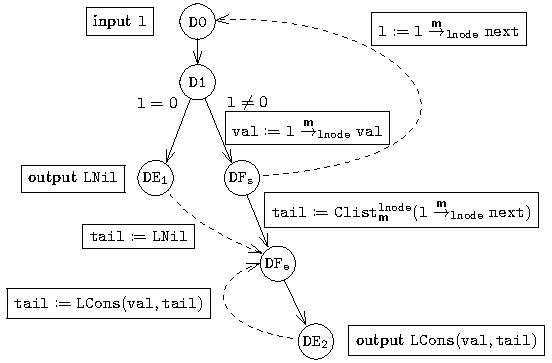
\includegraphics[scale=0.75]{chapters/figures/figClistCfg.pdf}
\caption{\label{fig:reconsProg}Reconstruction Program}
\end{subfigure}%
&
\begin{subfigure}[b]{0.50\textwidth}
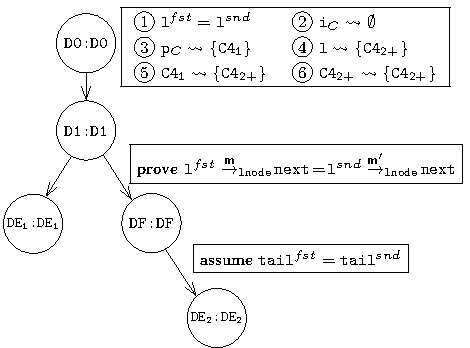
\includegraphics[scale=0.75]{chapters/figures/figClistProductCfg.pdf}
\caption{\label{fig:reconsPCFG}Recons-PCFG}
\end{subfigure}%
%&
%\begin{subfigure}[b]{0.17\textwidth}
%\includegraphics[scale=0.8]{figMallocPointsToGraph.pdf}
%\caption{\label{xxx}XXX}
%\end{subfigure}%
\\
\end{tabular}
\vspace{-8px}
\caption{\label{fig:recons}The reconstruction program and the recons-PCFG for {\tt Clist$^{lnode}_m({\tt l_{C}})$}. In \cref{fig:deconsProg}, {\tt D0} represents the unrolling procedure entry node, and the square boxes show the transfer functions of the unrolling procedure (\cref{eqn:clist}). The dashed edges represent a recursive function call. In \cref{fig:reconsPCFG}, the square box to the right of node {\tt D0:D0} contains the inferred invariants for this recons-PCFG.}
\vspace{-8px}
\end{figure}


The reconstruction
program and the recons-PCFG for our {\tt Clist} example
are shown in \cref{fig:decons}.
To check bisimulation
between the programs that deconstruct
${\tt Clist}_m^{{\tt lnode}}({\tt l}_C)$
and ${\tt Clist}_{m'}^{{\tt lnode}}({\tt l}_C)$, the recons-PCFG
correlates one unrolling of the first
program
with one
unrolling of the second program.
An unrolling of each reconstruction
program is based on the unrolling procedure in \cref{eqn:clist}.
Thus, the PC-transition correlations of both programs
are trivially obtained
by unifying the unrolling procedure with itself. A node
is created in the recons-PCFG that
encodes the correlation of the entries of the unrolling procedure in
both programs, we call this node the {\em recursive-node} in the
recons-PCFG, e.g., the
recursive node in \cref{fig:reconsPCFG} is {\tt D0:D0}. A recursive
call becomes a back-edge in the recons-PCFG that terminates at the
recursive-node.
A candidate
invariant at the recursive-node
is obtained by equating the pair of corresponding
{\tt l}$_C$ variables across the first and second
programs, i.e.,
${\tt l}^{fst}_C={\tt l}^{snd}_C$.
At the start of
both reconstruction
programs, ${\tt l}^{fst}_C={\tt l}^{snd}_C={\tt l}^{start}_C$
--- the
same ${\tt l}^{start}_C$ is passed to both reconstruction
programs, only the memory states $m$ and $m'$ are different.
The bisimulation check thus involves checking that
if the invariant
${\tt l}^{fst}_C={\tt l}^{snd}_C$
holds at the recursive-node,
then during one iteration of the unrolling procedure
in both programs:
\begin{enumerate}
\item The \underline{if} condition
({\tt l$^{fst}_C=0$}) in the first program
is equal to the corresponding \underline{if}
condition ({\tt l$^{snd}_C=0$}) in the
second program.
\item If the \underline{if} condition
evaluates to false in both programs, then
the observable values (that are used in the
construction of the list) are equal, i.e.,
$(({\tt l}^{fst}_C\neq 0)\land({\tt l}^{snd}_C\neq 0))\Rightarrow (\structPointer{{\tt l}^{fst}_C}{m}{s}{val}=
\structPointer{{\tt l}^{snd}_C}{m'}{\tt lnode}{val})$.
\item If the \underline{if} condition
evaluates to false in both programs, then
the invariant holds at the beginning
of the unrolling procedure invoked through the
recursive call.
This involves checking equality
of the arguments to the recursive call, i.e.,
$(({\tt l}^{fst}_C\neq 0)\land({\tt l}^{snd}_C\neq 0))\Rightarrow \structPointer{{\tt l}^{fst}_C}{m}{\tt lnode}{next}
=
\structPointer{{\tt l}^{snd}_C}{m'}{\tt lnode}{next}$.
\end{enumerate}
The first check succeeds due to the invariant
${\tt l}^{fst}_C={\tt l}^{snd}_C$.
For the second and third checks, we additionally
need to reason that the memory objects
$\structPointer{{\tt l}^{fst}_C}{m}{\tt lnode}{val}$ and
$\structPointer{{\tt l}^{fst}_C}{m}{\tt lnode}{next}$ cannot
alias with the writes (in $m'$ in \cref{eqn:memstore})
to the newly allocated objects
${\tt p}_C\xrightarrow[]{m}_{\mathrm{\tt lnode}}{\tt value}$
and
${\tt p}_C\xrightarrow[]{m}_{\mathrm{\tt lnode}}{\tt next}$.
This aliasing information is captured using a points-to analysis,
described in \cref{sec:pointsTo}.

Notice that a bisimulation check
between the reconstruction programs is significantly
easier than the top-level bisimulation check between \SpecL{}
and C programs: here,
the correlation of PC transitions is trivially
identified by unifying the unrolling procedure with itself, and
the candidate invariants
are obtained by equating each corresponding pair
of variables across
the two programs.

\subsubsection{Points-to Analysis}
\label{sec:pointsTo}
To reason about aliasing (as required during the bisimulation
check in \cref{sec:bisim}), we conservatively compute the
{\em may-point-to}
information for each program value using Andersen's algorithm \cite{andersen94programanalysis}.
The range of this computed
may-point-to function are {\em sets of region labels}, where
each region label identifies a set of memory objects.
The sets of memory objects identified by two distinct region
labels are necessarily disjoint. We write $p\pointsTo\{R_1,R_2\}$
to represent the condition that value $p$ may point to
an object belonging to one of the region labels $R_1$ or $R_2$ (but
may not point to any object outside of $R_1$ and $R_2$).

We populate the set of all region labels using the
{\em allocation
sites} of the program, i.e., PCs where a call to
{\tt malloc} exists, e.g., {\tt C4}
in \cref{fig:llAllocCIR} is an allocation site.
For each allocation site $A$, we create
two region labels: (1) the first region label, called $A_1$,
identifies the set of memory
objects that were allocated by the most recent execution of $A$. (2) The second
region label, called $A_{2+}$, identifies
the set of memory objects that were allocated by older (not the most
recent) executions of $A$.

For example, at the start of PC {\tt C7} in \cref{fig:llAllocCIR},
{\tt i}$_C\pointsTo{}\{\}$,
{\tt n}$_C\pointsTo{}\{{\tt C4}_1\}$,
and {\tt l}$_C\pointsTo{}\{{\tt C4}_{2+}\}$.
Because the may-point-to analysis determines the
sets of objects pointed-to by {\tt n}$_C$ and {\tt l}$_C$ to
be disjoint ($\{{\tt C4_{1}}\}$ vs. $\{{\tt C4_{2+}}\}$), any
memory accesses through {\tt n}$_C$ and {\tt l}$_C$
cannot alias at {\tt C7} (for an access
offset that is within the bounds of
the allocation size `{\tt sizeof lnode}').

The may-point-to information is computed not
just for scalar program values ({\tt n}$_C$,
{\tt l}$_C$, ...) but also for each region label.
For region labels $A1_{r1}$, $A2_{r2}$, $A3_{r3}$:
$A1_{r1}\pointsTo{}\{A2_{r2},A3_{r3}\}$ represents
the condition that the values (pointers) stored
in objects identified
by $A1_{r1}$ may point to an object identified by
either $A2_{r2}$ or $A3_{r3}$ (but not to any object
outside $A2_{r2}$ and $A3_{r3}$).
In \cref{fig:llAllocCIR}, at PC {\tt C7}, we
get
${\tt C4}_{1}\pointsTo{}\{{\tt C4}_{2+}\}$ and
${\tt C4}_{2+}\pointsTo{}\{{\tt C4}_{2+}\}$.
The condition
${\tt C4}_{1}\pointsTo{}\{{\tt C4}_{2+}\}$
holds because the {\tt next} pointer of the object
pointed-to by ${\tt n}_C$ (which
is a ${\tt C4}_1$ object) may point to
a {\tt C4}$_{2+}$ object (e.g., object pointed-to
by {\tt l}$_C$).
Similarly, ${\tt C4}_{2+}\pointsTo{}\{{\tt C4}_{2+}\}$
says that a pointer within a {\tt C4}$_{2+}$ object
may point to a {\tt C4}$_{2+}$
object (but not to a {\tt C4}$_1$ object).

\subsubsection{Transferring points-to information to the recons-PCFG}
\label{sec:pointsToAsInvariants}
Recall that
in \cref{sec:recursiveEqToBisim},
we reduce a validity check of the condition
${\tt Clist}_m^{{\tt lnode}}({\tt l}_C)
\indEq{} {\tt Clist}_{m'}^{{\tt lnode}}({\tt l}_C)$
to a bisimulation check. Also, recall
that we discharge the bisimulation check through the construction
of a recons-PCFG that compares the unrolling procedure with itself (executing
on memory states $m$ and $m'$).
During this bisimulation check, we need to prove
that for each execution
of the unrolling procedure, $\structPointer{{\tt l}_C}{m}{\tt lnode}{\{val,next\}}$
and $\structPointer{{\tt l}_C}{m'}{\tt lnode}{\{val,next\}}$\footnote{Here, we use the symbol {\tt l}$_C$ to
refer to equal values {\tt l}$^{fst}_C$ and
{\tt l}$^{snd}_C$.} are equal.
To successfully discharge these proof obligations, it suffices
to show ${\tt l}_C$ cannot alias with the memory writes that
distinguish $m$ from $m'$.

Our points-to analysis on
the C program determines that at PC {\tt C5} (the start of
the product-CFG edge {\tt (S3:C5)$\rightarrow$(S3:C3)} across which the proof
condition is being evaluated),
the pointer to the {\em head}
of the list, i.e., ${\tt l}^{start}_C$
points to {\tt C4}$_{2+}$. It also determines that the distinguishing
writes modify memory regions belonging to {\tt C4}$_1$. 
Further, we get ${\tt C4}_{2+}\pointsTo{}\{{\tt C4}_{2+}\}$ at PC {\tt C5}.
However,
notice that these determinations only rule out aliasing of the list-head with
the distinguishing writes. We also need to confirm non-aliasing
of the internal nodes of the linked list with the distinguishing
writes.
For this, we need to identify a points-to invariant,
{\tt l}$_C\pointsTo{}\{{\tt C4}_{2+}\}$, at the recursive-node
of the recons-PCFG
(shown in \cref{fig:reconsPCFG}).
To see why {\tt l}$_C\pointsTo{}\{{\tt C4}_{2+}\}$ is
an inductive invariant at the recursive-node:
\begin{itemize}
\item (Base case) The invariant holds
at entry to the recons-PCFG (because it holds for ${\tt l}^{start}_C$).
\item (Induction step) If ${\tt l}_C\pointsTo{}\{{\tt C4}_{2+}\}$
holds at the start of an unrolling procedure,
it also holds at the start of a recursive call to the
unrolling procedure. This
follows from ${\tt C4}_{2+}\pointsTo{}\{{\tt C4}_{2+}\}$ (points-to information at PC {\tt C5}),
which ensures that {\tt l$_C$->next} may point to only ${\tt C4}_{2+}$ objects.
\end{itemize}

To identify this points-to invariant, we run
our points-to analysis (the same analysis that is run
on the C program) on the reconstruction programs (\cref{fig:deconsProg})
before
comparing them for equivalence. The boundary
condition for the points-to analysis at the
entry node of the reconstruction
program (e.g., {\tt D0} in \cref{fig:decons}) is based on
the results of the points-to analysis
on $C$ at the PC where the proof obligation is being discharged (e.g., {\tt C5}
in our \cref{fig:llAllocC}). The points-to invariants
at a node {\tt (l$^{fst}_i$,l$^{snd}_j$)} of a recons-PCFG are
derived from the results of the points-to analysis on the individual
reconstruction programs at nodes l$^{fst}_i$ and l$^{snd}_j$
respectively.

During proof obligation discharge (e.g., during the bisimulation
check on recons-PCFG), the points-to invariants are encoded as SMT constraints.
This allows us to successfully
complete the bisimulation proof on the recons-PCFG, and
consequently successfully discharge the
proof obligation
$\{\phi_{{\tt S3:C5}}\}\\({\tt S3\rightarrow S5\rightarrow S3}, {\tt C5\rightarrow C3}) \{l_{S}\indEq{}Clist^{{\tt lnode}}_{m}(l_{C})\}$ in \cref{tab:llproductInv}.
The points-to analysis is described more formally
in \cref{sec:pointsToFormal}.

%Thus, as a part of the invariant inference procedure on the product-CFG
%for the decomposition programs, we also run our points-to analysis on the
%product-CFG to identify points-to invariants at the product-CFG
%nodes.  This improves precision, as shown in the example discussed
%above.
\vspace{-5px}
\subsubsection{Proof discharge algorithm for Category 3 obligations}
\label{sec:cat3summary}

\noindent
Before the start of an equivalence check, a points-to analysis is run on $C$.

During the equivalence check,
to discharge a Category 3 proof obligation $P: {\tt LHS}\Rightarrow{\tt RHS}$ (expressed
in first-order logic), we first replace the recursive
values of program $S$ in the {\tt RHS}
with lifted C values, based on the equalities present in the {\tt LHS}, to
obtain $P_2$.
This is followed by decomposition and RHS-breaking of $P_2$.
If the decomposition
fails, we evaluate $P$ to false (disproven) with a counterexample
that demonstrates the unification failure.

Upon successful decomposition, we
obtain several smaller proof obligations.
To
prove $P$, we require all these smaller proof
obligations to be provable. If any of these smaller proof obligations
is not provable, we are unable to prove $P$.  If we obtain a counterexample
to any of these smaller proof obligations, then that counterexample
also falsifies $P$.
Let $P_3$ represent any such smaller proof obligation. $P_3$, being
a decomposition clause,
must relate atomic expressions on the {\tt RHS}.
If $P_3$ relates two scalar values in the {\tt RHS}, then
it is
a Category 2 proof obligation and can be discharged
using the algorithm in \cref{sec:cat2algo}.

If $P_3$ relates two lifted
expressions (with the same lifting constructor) in
the {\tt RHS},
we check if the reconstruction
programs of the two lifted ADT values being
compared can be proven to be bisimilar (assuming that
{\tt LHS} holds at the correlated entry nodes
of the reconstruction programs).
To improve
the bisimulation
check's precision, we transfer the points-to information at the entry to the
reconstruction programs (obtained from {\tt LHS} which includes
from the points-to results of the C program at the
from-PC where the proof obligation is being discharged)
to the beginning of every iteration
of the unrolling procedure --- this is
achieved by running a points-to analysis
on the reconstruction programs.

These queries
generated by a bisimulation check are discharged
by a recursive call to the proof discharge procedure.
The depth of these recursive calls to the
proof discharge procedure is determined by
the maximum {\em recursion nest depth} (similar
to loop nest depth) of the decomposition
program.

If the bisimilarity check succeeds, the proof procedure returns
true for $P$.
If the bisimilarity check fails,
we imprecisely return false for $P$ (without a counterexample).

Finally, if $P_3$ neither
relates two scalar values, nor relates two
lifted expressions (with the same lifting constructor),
we imprecisely return false for $P$ (without a counterexample).

A more detailed discussion on algorithms introduced in this section
along with their pseudo-code is available in the thesis.
\chapter{Spec-to-C Equivalence Checker}
\label{sec:spectocalgo}
This chapter presents our automatic equivalence checker algorithm \toolName{}.
Given a \SpecL{} and a C program along with the input-output specification for each function-pair,
\toolName{} searches for a proof of equivalence between the CFGs of each \SpecL{} and C procedures: \sprog{} and \cprog{}.
Recall that CFGs represent deterministic programs and evidently, the C procedure is determinized during conversion to \cprog{}.
Hence, \toolName{} checks equivalence between a \SpecL{} procedure and the determinized C procedure.
A translation validator (such as the Counter tool \cite{oopsla20}) can be used to check equivalence between
the same determinized C procedure against its generated assembly.
By restricting the deterministic choices made by the C compiler to the same choices made during construction of \cprog{},
we can effectively establish end-to-end equivalence between a \SpecL{} procedure against its assembly.
We start with a dataflow formulation of the points-to analysis used as part of \toolName{} on \cprog{} as well as
deconstruction programs during discharge of type III proof obligations in \cref{sec:pointsToFormal}.
As stated in \cref{sec:contribs}, \toolName{} is based on three primary interdependent algortihms:
\curved{A1} an algorithm to incrementally construct a product-CFG by correlating program executions across
\sprog{} and \cprog{},
\curved{A2} an algorithm to identify inductive invariants at intermediate PCs in the (partially constructed)
product-CFG, and
\curved{A3} an algorithm for solving proof obligations generated by \curved{A1} and \curved{A2} algorithms.
We describe our counterexample-guided best-first search algorithm for construction of a product-CFG (\curved{A1}) in \cref{sec:searchalgo}.
This is followed by a dataflow formulation of our counterexample-guided invariant inference algorithm (\curved{A2}) in \cref{sec:invinferalgo}.
The previous chapter walked through our proof discharge algorithm (\curved{A3}) using examples, ending with
the pseudo-code of proof discharge algorithm (\cref{algo:proofSummary} in \cref{sec:proofsummary}).
In this chapter, we present pseudo-code for multiple subprocedures used as part of our proof discharge algorithm.
Additionally, we describe the process of encoding queries in SMT logic as well as recovering counterexamples from models returned by SMT solvers.

\begin{table}
\begin{center}
\caption{\label{tab:pointstoalgodfa}Dataflow Formulation of the Points-to Analysis}
\vspace{10px}
% \begin{footnotesize}
\begin{tabular}{|l|l|}
\hline
\Tstrut \Bstrut Domain &
\begin{tabular}{@{}l@{\hskip 12mm}l@{}}
$\Delta^{\cprog{}} : (\pseudoregs{}^{\cprog{}} \cup \memregions{}) \rightarrow 2^{\memregions{}}$ &
$\Delta^{\dprog{}} : (\pseudoregs{}^{\cprog{}} \cup \memregions{} \cup \pseudoregs{}^{\dprog{}}) \rightarrow 2^{\memregions{}}$ \\
\end{tabular} \\
\hline
\Tstrut \Bstrut Direction & Forward \\
\hline
Boundary Condition &
\begin{tabular}{@{}l@{\hskip 11mm}l@{}}
\multicolumn{2}{@{}l}{\Tstrut \Bstrut $\Delta_n$ for start node :}\\
$\Delta_n^{\cprog{}}(t) = \begin{dcases} \emptyset \ \ \  t \in \pseudoregs{}^{\cprog{}} \\ \memregions{} \ \ t \in \memregions{} \end{dcases}$ &
$\Delta_n^{\dprog{}}(t) = \begin{dcases} \Delta_{n_C}^{\cprog{}}(t) \ \  t \in (\pseudoregs{}^{\cprog{}} \cup \memregions{}) \\ \emptyset \ \ \ \ \ \ \ \ \ \  t \in \pseudoregs{}^{\dprog{}} \end{dcases}$ \\
\end{tabular} \\
\hline
\Tstrut \Bstrut Initialization to $\top$ & $\Delta_n$ for non-start nodes : $\Delta_n(t) = \emptyset \ \  t \in {\tt Domain}(\Delta_n)$ \\
\hline
\makecell[l]{\Tstrut Transfer function across \\
\Bstrut edge $e = (s \rightarrow d)$} &
$\Delta_d = f_e(\Delta_s)$ (described in \cref{sec:pointsToFormal}) \\
\hline
Meet operator $\otimes$ &
\makecell[l]{\Tstrut $\Delta_n \leftarrow \Delta^1_n \otimes \Delta^2_n$ \\
\Tstrut \Bstrut $\Delta_n(t) = \Delta^1_n(t) \cup \Delta^2_n(t) \ \  t \in {\tt Domain}(\Delta_n)$} \\
\hline
\end{tabular}
% \end{footnotesize}
\end{center}
\end{table}

\section{Points-to Analysis}
\label{sec:pointsToFormal}
Recall that in \cref{sec:reconsbisim}, we needed to reason about aliasing to successfully discharge a type III proof obligation.
These aliasing relationships are described in \cref{sec:pointsTo} and used in \cref{sec:pointsToAsInvariants} to
successfully discharge a type III proof obligation.
A points-to analysis is used to identify these relationships in \cprog{} as well as each deconstruction program \dprog{}.
\Cref{tab:pointstoalgodfa} presents a dataflow formulation of our points-to analysis.
We start by identifying the set \memregions{} of all region labels representing mutually non-overlapping
regions of the \cprog{} memory \mem{}.
For each call to {\tt malloc()} at PC $A$, we add $A_1$ and $A_{2+}$ to \memregions{}.
Recall that $A_1$ represents the region of memory returned by the {\em most recent} execution of $A$.
$A_{2+}$ represents the region of memory returned by older (i.e. all but most recent) executions of $A$.
$\memregions{} = \bigcup_{A} \{ A_1, A_{2+} \} \cup \{ \heapr{} \}$,
where \heapr{} is the region of memory \mem{} not covered by the labels associated with allocation sites.
Note that \memregions{} is computed globally i.e. in case $C$ consists of multiple procedures,
\memregions{} is identical for each and contains regions associated with allocation sites of {\tt malloc()}
calls for all procedures.

Let $\pseudoregs{}^{\cprog{}}$  be the set of all scalar pseudo-registers in \cprog{}.
We use a forward dataflow analysis to identify a may-point-to function
$\Delta^{\cprog{}}: (\pseudoregs{}^{\cprog{}} \cup \memregions{}) \mapsto 2^{\memregions{}}$ at each program point in \cprog{}.
For a deconstruction program \dprog{}, we are also interested in finding the may-point-to function for
all scalar pseudo-registers in \dprog{}, say $\pseudoregs{}^{\dprog{}}$.
Thus, the domain of the may-point-to function for \dprog{} ($\Delta^{\dprog{}}$) contains $\pseudoregs{}^{\dprog{}}$
in addition to the domain of $\Delta^{\cprog{}}$ i.e.
$\Delta^{\dprog{}}: (\pseudoregs{}^{\cprog{}} \cup \memregions{} \cup \pseudoregs{}^{\dprog{}}) \mapsto 2^{\memregions{}}$.
The '$\pointsTo$' operator introduced in \cref{sec:pointsTo} is called the {\em element-wise} may-point-to function
and is related to the may-point-to function $\Delta$ as follows: $p \pointsTo{} S \Leftrightarrow \Delta(p) = S$.

The meet operator is element-wise set-union e.g., $p \pointsTo{} S_1$ and $p \pointsTo{} S_2$
combines into $p \pointsTo{} S_1 \cup S_2$.
Evidently, the $\top$ value is the constant function that returns $\emptyset$.
At entry of \cprog{}, we conservatively assume that all memory regions may point to each other.
However, at entry of a deconstruction program \dprog{}, created during a proof obligation at product-CFG node $(n_S\!:\!n_C)$,
we use \cprog{}'s precomputed may-point-to function at $n_C$ ($\Delta^{\cprog{}}_{n_C}$)
to initialize the points-to relationships for all state elements of \cprog{} (i.e. $(\pseudoregs{}^{\cprog{}} \cup \memregions{})$).
This is a crucial step for proving equality of \cprog{} values under different memory states as seen in \cref{sec:pointsToAsInvariants}.

Next, we discuss the transfer function $f_e$ for our points-to analysis.
For an IR instruction ${\tt x} \coloneqq {\tt c}$, for constant {\tt c}, the
transfer function updates $\Delta({\tt x}) \coloneqq \emptyset$.
For instruction ${\tt x} \coloneqq {\tt y\ op\ z}$ (for some arithmetic or logical operator {\tt op}),
we update $\Delta({\tt x}) \coloneqq \Delta({\tt y}) \cup \Delta({\tt z})$.
For a load instruction ${\tt x} \coloneqq \memRead{\mem{}}{y}{T}$, we
update $\Delta({\tt x}) \coloneqq \bigcup_{t \in \Delta(y)} \Delta(t)$.
For a store instruction $\mem{} \coloneqq \memWrite{\mem{}}{x}{y}{T}$, for all
$t \in \Delta({\tt x})$, we update $\Delta(t) \coloneqq \Delta(t) \cup \Delta(y)$.
For a malloc instruction ${\tt x} \coloneqq {\tt malloc}_A()$
(where $A$ represents the allocation site), we perform the following steps (in order):
\begin{enumerate}
\item Convert all existing occurrences of $A_1$ to $A_{2+}$, i.e., for all $t \in (\pseudoregs{}^{\cprog{}} \cup \memregions{})$,
if $A_1 \in \Delta(t)$, then update $\Delta(t) \coloneqq (\Delta(t) \setminus \{ A_1 \}) \cup \{ A_{2+} \}$.
\item Update $\Delta({\tt x}) \coloneqq \{ A_1 \}$.
\item Update $\Delta(A_{2+}) \coloneqq \Delta(A_{2+}) \cup \Delta(A_1)$.
\item Update $\Delta(A_1) \coloneqq \emptyset$.
\end{enumerate}

For function calls, a {\em supergraph} is created by adding control flow edges
from the call-site to the procedure head (copying actual arguments to the formal arguments) and
from the procedure exit to the program point just after the
call-site (copying returned value to the variable assigned at the callsite),
e.g., in \cref{fig:clistdeconsCFG}, the dashed edges represent supergraph edges.

The allocation-site abstraction (with a bounded-depth call stack) is
known to be effective at disambiguating memory regions belonging to
different data structures
\cite{allocationSiteAbstraction82,allocationSiteAbstraction90,allocationSiteAbstraction06}.
In our work, we also need to reason about non-aliasing
of the most-recently allocated object (through a {\tt malloc} call) and
the previously-allocated objects (as in the \type{List}
construction example). The coarse-grained $\{1, 2+\}$
categorization of allocation recency is effective for such disambiguation.

\begin{figure}
\begin{algorithm}[H]
\begin{footnotesize}
\SetAlgoLined
\SetKwProg{Fn}{Function}{}{end}
\Fn{$bestFirstSearch(\sprog{},\cprog{},\mu)$}{
  $\pi_{init} \mapsfrom createInitProductCFG(\sprog{},\cprog{})$;\\
  $Q \mapsfrom \{ \pi_{init} \}$;\\
  \While{$Q \keyword{is\ not} empty$}{
    $\pi_{cur} \mapsfrom extractMostPromising(Q)$;\\
    ${\tt InferInvariantsAndCounterexamples}(\pi_{cur})$;\\
    \
    \uIf{$getPathsetToCorrelate(\cprog{},\pi_{cur}) = \cons{Found}(\xi_C)$}{
      \ForEach{$\xi_S \keyword{in} enumeratePathsetsInS(\sprog{},\xi_C,\mu)$}{
        $\pi_{next} \mapsfrom extendProductCFG(\pi_{cur},\xi_S,\xi_C)$;\\
        $Q \mapsfrom Q \cup \{ \pi_{next} \}$;\\
      }
    }
    \ElseIf{$productCFGRepresentsBisim(\pi_{cur})$}{
      \Return{$\cons{Found}(\pi_{cur})$};\\
    }
  }
  \Return{$\cons{NotFound}$};\\
}
\end{footnotesize}
\caption{\label{algo:search}Pseudocode for Best-First-Search Procedure for construction of Product-CFG}
\end{algorithm}
\end{figure}

\section{Counterexample-guided Product-CFG Construction}
\label{sec:searchalgo}
\toolName{} constructs a product-CFG incrementally to search for a bisimulation relation
between the \SpecL{} and C CFGs : \sprog{} and \cprog{}.
Multiple candidate product-CFGs are partially constructed during this search;
the search completes when one of these candidates yield an equivalence proof.

{\em Anchor nodes} are identified in \sprog{} and \cprog{}, and represents the
CFG nodes (i.e. IR PCs) being considered for correlation.
The algorithm ensures that every cycle in both \sprog{} and \cprog{} contains at least one anchor node.
The start and exit nodes are always anchor nodes.
Also, for every function call, the nodes just before and after its callsite are considered anchor nodes.
For example, in \cref{fig:llAllocCCFG}, \cpc{4} and \cpc{5} are anchor nodes around the call to {\tt malloc}.
The selected anchor nodes for the CFGs in \cref{fig:llAllocSpecIRCFG,fig:llAllocCCFG} are:
$\{ \spc{0},\spc{3},\spc{E} \}$ and $\{ \cpc{0}, \cpc{3}, \cpc{4}, \cpc{5}, \cpc{E} \}$ respectively.
For each anchor node in \cprog{}, our search algorithm searches for a correlated anchor node in \sprog{} --- if
a (partially constructed) product-CFG $\pi$ contains a product-CFG node  $(n_S\!:\!n_C)$, then $\pi$
correlates node $n_C$ in \cprog{} with node $n_S$ in \sprog{}.
The search procedure begins with a single partially-constructed product-CFG $\pi_{init}$.
$\pi_{init}$ contains exactly one node (\scpc{0}{0}) that encodes the correlation of the entry nodes
(i.e. \spc{0} and \cpc{0}) of \sprog{} and \cprog{}.

\subsection{Correlating Pathsets}
\label{sec:pathsetcorrel}
At each step of the incremental construction process, a node $(n_S\!:\!n_C)$ is chosen in a product-CFG $\pi$
and a 1-{\em pathset} $\xi_C$ in \cprog{} starting at $n_C$ (and ending at an anchor node in \cprog{}) is selected.
Then, we enumerate potentially correlated $\mu$-{\em pathsets} in \sprog{} for the pathset $\xi_C$ in \cprog{}.
A {\em pathset} $\xi$ is essentially a set of paths with the following additional properties:
(a) all paths $\rho \in \xi$ begin at the same node and terminate at the same node,
(b) all paths $\rho \in \xi$ are mutually-exclusive i.e. {\em at most} one of ${\tt pathcond}_\rho$ can be true.
A $\mu$-pathset $\xi$ is a pathset where each path $\rho \in \xi$ contains {\em at most} $\mu$ occurrences of any node.
$\mu$-pathsets are based on earlier work on the Counter tool \cite{oopsla20}\footnote{
Counter tool \cite{oopsla20} considers $(\mu,\delta)$-unrolled pathsets in its correlation search algorithm.
Our $\mu$-pathsets are a special case of $(\mu,\delta)$-unrolled pathsets where $\delta = \mu$.}
and helps improve the completeness of the bisimulation search
by attempting to correlate a set of \cprog{} paths with a set of \sprog{} paths,
where individual paths of \cprog{} and \sprog{} may be uncorrelated.
An example of such a scenario is depicted in \cref{sec:expstring}.
\Cref{sec:pathsethoaretriples} briefly discusses the techniques of handling Hoare triples (i.e. proof obligations)
involving pathsets.

Revisiting our incremental construction process, recall that we choose a 1-pathset $\xi_C$ in \cprog{}
and enumerate potentially correlated $\mu$-pathsets $\xi_S$ in \sprog{}.
Hence, $\mu$ represents the maximum number of iterations of a loop (in \sprog{}),
that may be correlated with a pathset in \cprog{} consisting of acyclic paths.
$\mu$ is a fixed parameter of the \toolName{} algorithm and is called the {\em unroll factor}.
For example, during construction of the product-CFG shown in \cref{fig:llAllocProductCFG},
say we select the product-CFG node (\scpc{3}{3}).
We choose the \cprog{} path(set) \cpath{3,4} and enumerate its potential correlations (i.e. $\mu$-pathsets in \sprog{} starting at \spc{3}):
$\epsilon$, \spath{3,5,3}, \ldots, $\pathset{S3,(\pathset{S5,S3})^{(\mu-1)}}$.
Importantly, for pathsets $\xi_S$ (in \sprog{}) and $\xi_C$ (in \cprog{}) to be considered for correlation,
they must originate and terminate at anchor nodes, i.e. the path \spath{3,5} is skipped during enumeration.
Moreover, the pathset $\xi_C$ may only contain anchor nodes as its source and destination.
Hence, the path \cpath{3,4,5} is not considered for $\xi_C$,
instead we attempt to correlate the subpaths \cpath{3,4} and \cpath{4,5} individually.

For each enumerated correlation possibility $(\xi_S,\xi_C)$, a separate product-CFG $\pi'$ is
created (by cloning $\pi$) and a new product-CFG edge $e=(\xi_S,\xi_C)$ is added to $\pi'$.
The head of the product-CFG edge $e$ is the (potentially newly added) product-CFG node representing
the correlation of the end-points of pathsets $\xi_S$ and $\xi_C$. For example, the node (\scpc{3}{4}) is added
to the product-CFG if it correlates pathsets $\epsilon$ and \cpath{3,4} starting at (\scpc{3}{3}).
Recall that, we consider $\epsilon$ as a candidate for $\xi_S$, but not $\xi_C$.
The algorithm ensures that no cycle in \cprog{} is correlated with $\epsilon$ in \sprog{}
(to preserve divergence discussed in \cref{sec:bisim}).
For each node $n$ in a product-CFG $\pi$, we maintain a small number of
concrete machine state pairs (of \sprog{} and \cprog{}).
The concrete machine state pairs at $n$ are obtained as counterexamples to an unsucessful proof
obligation \hoareTriple{\phi_s}{s \rightarrow d}{\phi_d} (for some edge $s \rightarrow d$ and node $d$ in $\pi$).
Thus, by construction, these counterexamples represent concrete state pairs that may potentially occur
at $n$ during the lockstep execution encoded by $\pi$.

\subsection{Best-First Ranking of Partial Product-CFGs}
\label{sec:rankproductcfg}
To evaluate the promise of a possible correlation $(\xi_S,\xi_C)$ starting at node $n$
in product-CFG $\pi$, we examine the execution behaviour of the counterexamples at $n$ on
the product-CFG edge $e=(s\rightarrow d)=(\xi_S,\xi_C)$.
If the counterexamples ensure that the machine states remain related at $d$,
then that candidate correlation is ranked higher.
This ranking criterion is based on prior work \cite{oopsla20}.
A best-first search (BFS) procedure based on this ranking criterion is used to incrementally construct
a product-CFG (starting from $\pi_{init}$).
For each intermediate candidate product-CFG $\pi$ generated during this search procedure,
an automatic invariant inference procedure (discussed next in \cref{sec:invinferalgo}) is
used to identify invariants at all the nodes in $\pi$.
The counterexamples obtained from the proof obligations generated by this invariant inference
procedure are added to the respective nodes in $\pi$; these counterexamples help rank
future correlations starting at those nodes.

If after invariant inference, we realize that an intermediate candidate product-CFG $\pi_1$
is not promising enough, we backtrack and choose another candidate product-CFG $\pi_2$
and explore the potential correlations that can be added to $\pi_2$.
Thus, a product-CFG is constructed one edge at a time.
If at any stage, a product-CFG $\pi$ contains correlations for every path in \cprog{}
and invariants ensure equal observables (i.e. \post{} holds at correlated exit nodes),
we have successfully shown equivalence.
This counterexample-guided BFS procedure is similar to the one described in prior work on
the Counter algorithm \cite{oopsla20}.

\subsection{Correlation in the Presence of Function Calls}
\label{sec:correlfcalls}
Recall that \sprog{} and \cprog{} may make function calls (including self calls),
e.g., allocation of memory in C, recursive traversal of a tree data structure.
Recall that the nodes just before and after a function call are always considered anchor nodes.
Calls to memory allocation functions in \cprog{} (i.e. {\tt malloc}) are handled by correlating
the function call edge with the empty path ($\epsilon$) in \sprog{}.
For example, in the product-CFG shown in \cref{fig:llAllocProductCFG}, the {\tt malloc} edge \cpath{4,5} in \cprog{}
is correlated with $\epsilon$ in \sprog{}.

For all other calls, our correlation algorithm (in \cref{sec:searchalgo}) ensures that the anchor nodes
around such a callsite are correlated one-to-one across both procedures.
For example, let there be a call to procedure $\delta$ in \sprog{} at PC $n_S$, i.e. $n_S$ is the call-site.
Let us denote the program point just after this call-site as $n'_S$.
Let {\tt args}$_{n_S}$ represent the values of the actual arguments of this function call (at $n_S$).
Let {\tt ret}$_{n'_S}$ represent the value returned by this function call (at $n'_S$).
Similarly, for a procedure call $\delta$ in \cprog{}, let $n_C$, $n'_C$, {\tt args}$_{n_C}$ and {\tt ret}$_{n'_C}$
represent the function call-site, program point just after the call-site,
the values of the actual arguments and the value returned respectively.
Our algorithm ensures that the only correlation possible in a product-CFG $\pi$ for these program points are
$(n_S:n_C)$ and $(n'_S:n'_C)$.

We utilize the user-supplied input-output specification for $\delta$ (say $(\pre{}_{\delta},\post{}_{\delta})$)
to obtain the desired invariants at nodes $(n_S:n_C)$ and $(n'_S:n'_C)$ in the product-CFG.
A successful proof must {\em ensure} that $Pre_{\delta}$({\tt args}$_{n_S}$,{\tt args}$_{n_C}$) holds at $(n_S:n_C)$.
Further, the proof can {\em assume} that $Post_{\delta}$({\tt ret}$_{n'_S}$,{\tt ret}$_{n'_C}$) holds at $(n'_S:n'_C)$.
Note that {\tt args}$_{n_C}$ and {\tt ret}$_{n'_C}$ includes the \cprog{} memory states
$\mem{}_{n_C}$ (at $n_C$) and $\mem{}_{n'_C}$ (at $n'_C$) respectively.
Thus, for function calls, we inductively prove the precondition (on the arguments) at $(n_S:n_C)$
and assume the postcondition (on the returned values) at $(n'_S:n'_C)$.

\begin{table}[H]
\begin{center}
\caption{\label{tab:dataflow_formulation}Dataflow formulation for the Invariant Inference Algorithm.}
\setlength{\belowcaptionskip}{-30pt}
\begin{footnotesize}
\begin{tabular}{|l|l|}
\hline
Domain &
\makecell[c]{
\ldelim\{{2}{3mm}{\footnotesize \ \  $\phi_n$ is a conjunction of predicates drawn from\ \ }\rdelim\}{2}{3mm} \\ \ {\footnotesize grammar in \ref{fig:invGrammar}, $\Gamma_n$ is a set of counterexamples}} \\
\hline
Direction & Forward\\
\hline
\makecell[l]{Transfer function across \\ edge $e=(s\rightarrow d)$} & $(\phi_d,\Gamma_d) = f_e(\phi_s,\Gamma_s)$ (\cref{algo:tf})\\
\hline
\begin{tabular}{@{}l@{}}
Meet operator $\otimes$\\
{\footnotesize $(\phi_n,\Gamma_n) \leftarrow (\phi^1_n,\Gamma^1_n) \otimes (\phi^2_n,\Gamma^2_n)$}\\
\end{tabular}
& $\Gamma_n \leftarrow \Gamma^1_n\cup \Gamma^2_n$, \ \ \ \ \ \ \ \ $\phi_n \leftarrow \mathrm{\it StrongestInvCover}(\Gamma_n)$\\
\hline
Boundary condition & {\tt out[$n^{start}$]} = {\tt $(Pre,\Gamma_{n^{start}})$}\ \ \ \ \ \\
\hline
Initialization to $\top$ & {\tt in[$n$] = $($False,$\{\})$} for all non-start nodes\\
\hline
\end{tabular}
\end{footnotesize}
\end{center}
\end{table}
\vspace{-10px}
\begin{figure}[H]
\begin{center}
\begin{subfigure}{.58\textwidth}
\begin{algorithm}[H]
\begin{footnotesize}
\SetAlgoLined
\SetKwProg{Fn}{Function}{}{end}
\Fn{$f_e(\phi_s, \Gamma_s)$}{
  $\Gamma^{can}_{d} \mapsfrom \Gamma_{d} \cup {\tt exec}_e(\Gamma_s)$;\\
  $\phi^{can}_{d} \mapsfrom \mathrm{\it StrongestInvCover}(\Gamma^{can}_{d})$;\\
  \While{{\tt SAT$(\neg(\{\phi_s\} (e) \{\phi^{can}_{d}\}), \gamma_s)$}}
  {
    $\gamma_{d} \ \ \ \ \mapsfrom {\tt exec}_e(\gamma_s)$;\\
    $\Gamma^{can}_{d} \mapsfrom \Gamma^{can}_{d}\cup\gamma_{d}$;\\
    $\phi^{can}_{d} \mapsfrom \mathrm{\it StrongestInvCover}(\Gamma^{can}_{d})$;\\
  }
  \Return{$(\phi^{can}_{d}, \Gamma^{can}_{d})$;}\\
}
\end{footnotesize}
\end{algorithm}
\caption{\label{algo:tf} Transfer function $f_e$ across
edge $e=(s\rightarrow d)$.}
\end{subfigure}%
\hfill
\rulesep
\hfill
\begin{subfigure}{.40\textwidth}
\begin{center}
\begin{footnotesize}
\begin{tabular}{p{0.45cm}p{0.15cm}l}
${Inv}$ & $\rightarrow$ & $\sum_{i}{c_i v_i}=c$ $|$ $v_1 \odot v_2$  \\
% & $|$ & $v_1 \odot v_2$ \\
& $\ \ |$ & $\alpha_S = {\tt liftC}_m(v^C \dots)$ \\
\end{tabular}
\end{footnotesize}
\end{center}
\vspace{-10px}
\caption{\label{fig:invGrammar}\footnotesize Predicate grammar for constructing invariants. $v$ represents a bitvector variable in either $S$ or $C$. $c$ represents a bitvector constant. $\odot$ $\in$ $\{<,\leq\}$. $\alpha_S$ represents an ADT variable in \SpecL{}. $v^{C}$ represents a bitvector variable in $C$. $m$ represents the current $C$ memory state.}
\end{subfigure}%
\caption{Transfer function $f_e$ and Predicate grammar $Inv$ for invariant inference dataflow analysis in \cref{tab:dataflow_formulation}.
Given invariants ($\phi_{s}$) and counterexamples ($\Gamma_{s}$) at node $s$,
$f_e$ returns the updated
invariants ($\phi_{d}$) and counterexamples ($\Gamma_{d}$) at
node $d$.
{\em StrongestInvCover($\Gamma$)} computes the strongest invariant cover for counterexamples $\Gamma$.
{\tt exec$_e$($\Gamma$)} (concretely) executes
counterexamples $\Gamma$ over edge $e$.
{\tt SAT($\phi$, $\gamma$)} determines
the satisfiability of $\phi$; if satisfiable, the models (counterexamples) are returned in output parameter $\gamma$.}
\end{center}
\end{figure}

\section{Invariant Inference and Counterexample Generation}
\label{sec:invinferalgo}
We formulate our counterexample-guided invariant inference algorithm as a dataflow analysis
as shown in \cref{tab:invinferalgodfa}.
The invariant inference procedure is responsible for inferring invariants $\phi_n$ at each intermediate
node $n$ of a (partially constructed) product-CFG, while also generating a set of counterexamples
$\Gamma_n$ that represents the potential concrete machine states at $n$.

Given the invariants and counterexamples at node $s$: ($\phi_s,\Gamma_s$),
the transfer function initializes the new candidate set of counterexamples at $d$ ($\Gamma^{can}_{d}$)
with the current set of counterexamples at $d$ ($\Gamma_{d}$) {\em union}-ed with
the counterexamples obtained by executing $\Gamma_s$ on edge $e$ (through {\tt exec}$_e$).
The candidate invariant at $d$ ($\phi^{can}_d$) is computed as the strongest cover
of $\Gamma^{can}_{d}$ ($StrongestInvCover()$).
At each step, the transfer function attempts to prove $\{\phi_s\} (e) \{\phi^{can}_d\}$
(through a call to $Prove()$).
If the proof succeeds ($Prove()$ returns \cons{True}), the candidate invariant $\phi^{can}_d$ is returned along with
the counterexamples $\Gamma^{can}_d$ learned so far.
Otherwise, $Prove()$ returns $\cons{False}(\gamma_s)$.
The candidate invariant $\phi^{can}_d$ is weakened using the counterexamples obtained
(i.e. $\gamma_s$) and the proof attempt is repeated.

The candidate invariants are drawn from the predicate grammar \invgrammar{} shown in \cref{fig:invinfergrammar}.
In addition to affine and inequality relations between bitvectors in \sprog{} and \cprog{},
\invgrammar{} supports \recursiveRelations{} between an ADT variable in \sprog{} and a lifted expression in \cprog{}.
The candidate lifting constructors of the form \lift{lift}{\mem{}}{T} (where \mem{} is the current
memory state in \cprog{}) are derived from the lifting constructors
present in the precondition \pre{} and the postcondition \post{}, as supplied by the user.
More sophisticated strategies for inference of new lifting constructors is left as future work.

$StrongestInvCover()$ for affine relations involve
identifying the basis vectors of the kernel of the
matrix formed by the counterexamples in the bitvector
domain \cite{esop05,semalign}.
For inequality relations, $StrongestInvCover(\Gamma)$
returns {\em true} (i.e. the weakest invariant) iff any counterexample in $\Gamma$ evaluates the
relation to false --- this effectively simulates the Houdini approach \cite{houdini}.
Similarly, in case of a \recursiveRelation{} $l_1 \indEq{} l_2$, $StrongestInvCover(\Gamma)$
returns {\em true} iff any counterexample in $\Gamma$ evalutes its $\eta$-depth over-approximation
$l_1 \indEqDepth{\eta} l_2$ to false (effectively falsifying a weaker condition), where $\eta$ is a fixed parameter of the algorithm.

\section{More on Proof Discharge Algorithm}
\label{sec:proofalgo}

\subsection{Handling Proof Obligations On Pathsets}
\label{sec:pathsethoaretriples}
Recall that our correlation algorithm attempts to correlate pathsets (instead of paths) between \sprog{} and \cprog{}.
Evidently, each edge of a (possibly partial) product-CFG $\pi$ is associated with a pair of pathsets $(\xi_S,\xi_C)$.
Proof obligations originating across a product-CFG edge $e[s \rightarrow d]=(\xi_S,\xi_C)$ are of
the form \hoareTriple{\phi_s}{\xi_S,\xi_C}{\phi_d}.
A Hoare triple of the above form can be broken down into a conjunction of Hoare triples involving purely paths as follows:

\begin{equation}
\label{eqn:hoaretriplepathset}
\hoareTriple{\phi_s}{\xi_S,\xi_C}{\phi_d} \Leftrightarrow \bigwedge_{\substack{\rho_S \in \xi_S \\ \rho_C \in \xi_C}} \hoareTriple{\phi_s}{\rho_S,\rho_C}{\phi_d}
\end{equation}

Recall that our proof discharge algorithm requires that proof obligations satisfy the conjunctive \recursiveRelation{} property (defined in \cref{sec:proofalgoprops}).
If the original proof obligation \hoareTriple{\phi_s}{\xi_S,\xi_C}{\phi_d} satisfies this property, so does each of the smaller
proof obligation \hoareTriple{\phi_s}{\rho_S,\rho_C}{\phi_d}.
Hence, the proof discharge algorithm presented in \cref{sec:examples} is capable of handling these smaller proof obligations
and by \cref{eqn:hoaretriplepathset}, also the original proof obligations.
If $|\xi|$ represents the number of paths in a pathset $\xi$, the proof obligation \hoareTriple{\phi_s}{\xi_S,\xi_C}{\phi_d} results
in $|\xi_S| \times |\xi_C|$ smaller proof obligations.
In practice, the number of paths in \sprog{} that are correlated with a path in \cprog{} is quite low
and consequently, most of these proof obligations usually end up with a {\tt false} \lhs{} when lowered to
first-order logic (through \cref{eqn:firstOrderFormula}), due to the presence of {\tt pathcond}$_{\rho_S}$ and {\tt pathcond}$_{\rho_C}$.
Our proof discharge procedure begins with an attempt to disprove \lhs{} (overapproximated in case of \recursiveRelations{}),
which trivially resolves the smaller proof obligations involving uncorrelated paths to {\tt true}.

\subsection{Canonicalization Procedure}
\label{sec:canonicalalgo}

\begin{figure}[H]
\begin{algorithm}[H]
\begin{footnotesize}
\SetAlgoLined
\SetKwProg{Fn}{Function}{}{end}
\Fn{$Canonicalize(e)$}{
  $\hat{e} \mapsfrom e$;\\
  \While{$e \keyword{contains} e' = \prodAccess{e_1}{a^i} \keyword{where} e_1 \keyword{is} foldable$}{
    \uIf{$e_1 = V_1^{(n)}(e_1^1,e_1^2,\dots,e_1^n)$}{
      $\hat{e} \mapsfrom \subst{\hat{e}}{e'}{e_1^i}$;\\
    }
    \uElseIf{$e_1 = $ \sumIf{c_1} \sumThen{V_1^{(n)}(e_1^1,e_1^2,\dots,e_1^n)} \sumElse{e_1^{\tt el}}}{
      \lIf{$V_1^{(n)} \keyword{contains} {\tt a^i}$}{$\hat{e} \mapsfrom \subst{\hat{e}}{e'}{e_1^i}$}
      \lElse{$\hat{e} \mapsfrom \subst{\hat{e}}{e'}{\prodAccess{e_1^{\tt el}}{a^i}}$}
    }
    \Else($e_1 = \lifted{lift}{\mem{}}{T}{e^1,e^2,\dots,e^n}$){
      $\hat{e} \mapsfrom \subst{\hat{e}}{e'}{\prodAccess{rewrite(e_1)}{a^i}}$;\\
    }
  }
  \While{$e \keyword{contains} e' = \sumIs{e_1}{\mathnormal{V_2^{(m)}}} \keyword{where} e_1 \keyword{is} foldable$}{
    \uIf{$e_1 = V_1^{(n)}(e_1^1,e_1^2,\dots,e_1^n)$}{
      \lIf{$V_1^{(n)} = V_2^{(m)}$}{$\hat{e} \mapsfrom \subst{\hat{e}}{e'}{true}$}
      \lElse{$\hat{e} \mapsfrom \subst{\hat{e}}{e'}{false}$}
    }
    \uElseIf{$e_1 = $ \sumIf{c_1} \sumThen{V_1^{(n)}(e_1^1,e_1^2,\dots,e_1^n)} \sumElse{e_1^{\tt el}}}{
      \lIf{$V_1^{(n)} = V_2^{(m)}$}{$\hat{e} \mapsfrom \subst{\hat{e}}{e'}{c_1}$}
      \lElse{$\hat{e} \mapsfrom \subst{\hat{e}}{e'}{\neg c_1 \land (\sumIs{e_1^{\tt el}}{\mathnormal{V_2^{(m)}}})}$}
    }
    \Else($e_1 = \lifted{lift}{\mem{}}{T}{e^1,e^2,\dots,e^n}$){
      $\hat{e} \mapsfrom \subst{\hat{e}}{e'}{\prodAccess{rewrite(e_1)}{a^i}}$;\\
    }
  }
  \Return{$\hat{e}$};
}
\end{footnotesize}
\caption{\label{algo:canonical}Pseudo-code for Canonicalization Procedure}
\end{algorithm}
\end{figure}

\Cref{algo:canonical} shows the pseudo-code for the canonicalization procedure.
$Canonicalize(e)$ is responsible for converting an expression $e$ to its canonical form $\hat{e}$ (introduced in \cref{sec:unifyandrewrite}).
Recall that a pseudo-variable is an expression of the form $\prodAccess{v}{a_1,a_2,.,a_n}$, where $v$ is a variable.
Also recall that, an expression $e$ is canonical iff each {\em accessor} and {\em sum-is} expression operate on a pseudo-variable.
An ADT expression with a data constructor, a lifting constructor or the \sumDtor{}-operator at its top-level, is called a {\em foldable} expression.
$Canonicalize(e)$ iteratively folds each {\em accessor} and {\em sum-is} subexpressions of $e$ that operate on a foldable argument.
Thus, $Canonicalize(e)$ returns an expression where none of the {\em accessor} or {\em sum-is} subexpressions is foldable.
This condition entails the requirements of the canonical form.
For example, $a + \prodAccess{\cons{LCons}(b,l)}{tail,val}$ and $\sumIs{\lifted{list}{\mem{}}{lnode}{p}}{LNil}$
canonicalizes to $a + \prodAccess{l}{val}$ and $(p = 0)$ respectively.

\subsection{Unification Procedure}
\label{sec:unifalgo}

\begin{figure}
\begin{algorithm}[H]
\begin{footnotesize}
\SetAlgoLined
\SetKwProg{Fn}{Function}{}{end}
\Fn{$\theta(p_1,e_1,p_2,e_2)$}{
  \uIf{$e_1 \keyword{is} atomic$}{
    \Return{$\cons{Succ}(\{ \corrtuple{p_1}{e_1}{p_2}{e_2} \})$};
  }
  \uElseIf{$e_2 \keyword{is} atomic$}{
    \Return{$\cons{Succ}(\{ \corrtuple{p_2}{e_2}{p_1}{e_1} \})$};
  }
  \uElseIf{$e_1 = V_1^{(n)}(e_1^1,e_1^2,\dots,e_1^n) \keyword{and} e_2 = V_2^{(m)}(e_2^1,e_2^2,\dots,e_2^m)$}{
    \If{$V_1^{(n)} \neq V_2^{(m)}$}{
      \Return{$\cons{Fail}$};
    }
    \Return{$\bigsqcup_{i \in [1,n]} \theta(p_1,e_1^i,p_2,e_2^i)$};
  }
  \uElseIf{$e_1 = V_1^{(n)}(e_1^1,e_1^2,\dots,e_1^n) \keyword{and} e_2 = $ \sumIf{c_2} \sumThen{e_2^{\tt th}} \sumElse{e_2^{\tt el}}}{
    $R^{\tt th} \mapsfrom \theta(p_1,true,p_2,c_2) \sqcup \theta(p_1,e_1,p_2 \oland c_2, e_2^{\tt th})$;\\
    \lIf{$R^{\tt th} = \cons{Succ}(S)$}{\Return{$\cons{Succ}(S)$}}
    $R^{\tt el} \mapsfrom \theta(p_1,true,p_2,\neg c_2) \sqcup \theta(p_1,e_1,p_2 \oland \neg c_2, e_2^{\tt el})$;\\
    \lIf{$R^{\tt el} = \cons{Succ}(S)$}{\Return{$\cons{Succ}(S)$}}
    \Return{$\cons{Fail}$};
  }
  \uElseIf{$e_1 = $ \sumIf{c_1} \sumThen{e_1^{\tt th}} \sumElse{e_1^{\tt el}} $\keyword{and} e_1 = V_2^{(m)}(e_2^1,e_2^2,\dots,e_2^m)$}{
    $R^{\tt th} \mapsfrom \theta(p_1,c_1,p_2,true) \sqcup \theta(p_1 \oland c_1,e_1^{\tt th},p_2, e_2)$;\\
    \lIf{$R^{\tt th} = \cons{Succ}(S)$}{\Return{$\cons{Succ}(S)$}}
    $R^{\tt el} \mapsfrom \theta(p_1,\neg c_1,p_2,true) \sqcup \theta(p_1 \oland \neg c_2,e_1^{\tt el},p_2, e_2)$;\\
    \lIf{$R^{\tt el} = \cons{Succ}(S)$}{\Return{$\cons{Succ}(S)$}}
    \Return{$\cons{Fail}$};
  }
  \Else($e_1 = $ \sumIf{c_1} \sumThen{e_1^{\tt th}} \sumElse{e_1^{\tt el}} $\keyword{and} e_2 = $ \sumIf{c_2} \sumThen{e_2^{\tt th}} \sumElse{e_2^{\tt el}}){
    $R_1 \mapsfrom \theta(p_1,c_1,p_2,c_2)$;\\
    $R_2 \mapsfrom \theta(p_1 \oland c_1, e_1^{\tt th}, p_2 \oland c_2, e_2^{\tt th})$;\\
    $R_3 \mapsfrom \theta(p_1 \oland \neg c_1, e_1^{\tt el}, p_2 \oland \neg c_2, e_2^{\tt el})$;\\
    \Return{$R_1 \sqcup R_2 \sqcup R_3$};
  }
}
\end{footnotesize}
\caption{\label{algo:unification}Pseudocode for Unification Procedure}
\end{algorithm}
\end{figure}

\Cref{algo:unification} shows the pseudo-code for the unification algorithm introduced in \cref{sec:unifyandrewrite}.
$\theta(p_1,e_1,p_2,e_2)$ is responsible for unifying expressions $e_1$ and $e_2$ under the expression path
conditions $p_1$ and $p_2$ respectively.
$\theta$ either fails to unify with the \cons{Fail} output, or it successfully returns $\cons{Succ}(S)$, where $S$
is the set of correlation tuples that relate (a) either two atomic expressions, or (b) an atom with an non-atomic expression.
$\theta(p_1,e_1,p_2,e_2)$ terminates when one of $e_1$ and $e_2$ is an atomic expression.
In case both $e_1$ and $e_2$ contains a data constructor at their top-level, 
$\theta$ attempts to recursively unify the data constructors and their corresponding children.
If exactly one of $e_1$ and $e_2$ is a \sumDtor{} expression,
$\theta$ attempts to unify both branches of \sumDtor{} (along with the path conditions) with the other expression
and return whichever succeeds.
If both $e_1$ and $e_2$ are \sumDtor{} expressions, $\theta$ attempts to recursively unify their children.
$\theta$ uses the $\sqcup$ -operator to combine the results of successive self-calls.
$A \sqcup B$ is equal to $\cons{Succ}(S_1 \cup S_2)$ if $A = \cons{Succ}(S_1)$ and $B = \cons{Succ}(S_2)$;
otherwise (if one of $A$ and $B$ is \cons{Fail}), $A \sqcup B = \cons{Fail}$.
Additionally, for a \sumDtor{} expression with \underline{\tt if} condition $c$, $c$ is well-formed under the expression path condition.
Hence, when conjuncting $c$ to the expression path condition, we use an `ordered and' operator \oland;
$e_1 \oland e_2$ is equivalent to $e_1 \land (e_1 \rightarrow e_2)$.

\subsection{Iterative Unification and Rewriting Procedure}
\label{sec:unifyandrewritealgo}

\begin{figure}[H]
\begin{algorithm}[H]
\begin{footnotesize}
\SetAlgoLined
\SetKwProg{Fn}{Function}{}{end}
\Fn{$\Theta(p_a,e_a,p_b,e_b)$}{
  $R \mapsfrom \emptyset$;\\
  $S \mapsfrom \theta(p_a,e_a,p_b,e_b)$;\\
  \lIf{$S = \cons{Fail}$}{\Return{$\cons{Fail}$}}
  \ForEach{$\corrtuple{p_1}{a_1}{p_2}{e_2} \keyword{in} S$}{
    \uIf{$e_2 \keyword{is} atomic$}{
      $R \mapsfrom R \cup \{ \corrtuple{p_1}{a_1}{p_2}{e_2} \}$;\\
    }
    \Else{
      $e_1 \mapsfrom rewrite(a_1)$;\\
      $R_1 \mapsfrom \Theta(p_1,e_1,p_2,e_2)$;\\
      \lIf{$R_1 = \cons{Fail}$}{\Return{$\cons{Fail}$}}
      $R \mapsfrom R \cup R_1$;\\
    }
  }
  \Return{$\cons{Succ}(R)$};
}
\end{footnotesize}
\caption{\label{algo:unifyandrewrite}Pseudo-code for Iterative Unification and Rewriting Procedure}
\end{algorithm}
\end{figure}

\Cref{algo:unifyandrewrite} shows the pseudo-code for the iterative unification and rewriting procedure
introduced in \cref{sec:unifyandrewrite}.
$\Theta(p_a,e_a,p_b,e_b)$ is responsible for unifying expressions $e_a$ and $e_b$ under the expression
path conditions $p_a$ and $p_b$ respectively.
$\Theta$ either fails to unify with the \cons{Fail} output, or it successfully returns $\cons{Succ}(S)$, where $S$
is the set of correlation tuples that relate {\em only} atomic expressions.
$\Theta$ attempts to iteratively (a) unify the expressions (through a call to the unification procedure $\theta$ in \cref{sec:proofalgo}),
and (b) perform rewriting (of atom $a_1$ for those correlation tuples \corrtuple{p_1}{a_1}{p_2}{e_2} where $e_2$ is non-atomic), followed by
a recursive call to $\Theta$.
For example, the unification of $l_1$ and $\cons{LCons}(42, \lifted{list}{\mem{}}{lnode}{l_2})$
yields the correlation tuples:
$\corrtuple{true}{\sumIs{l_1}{LCons}}{true}{true}$, $\corrtuple{\sumIs{l_1}{LCons}}{\prodAccess{l_1}{val}}{true}{42}$ and
$\corrtuple{\sumIs{l_1}{LCons}}{\prodAccess{l_1}{tail}}{true}{\lifted{list}{\mem{}}{lnode}{l_2}}$.

\subsection{Decomposition Procedure for Recursive Relations}
\label{sec:decomposealgo}

\begin{figure}[t!]
\begin{algorithm}[H]
\begin{footnotesize}
\DontPrintSemicolon
\everypar={\nl}
\SetAlgoLined
\SetKwProg{Fn}{Function}{}{end}
\Fn{$decompose(l_1,l_2)$}{
  $P \mapsfrom true$\\
  $\hat{l}_1 \mapsfrom {\tt canonicalize}(l_1)$\\
  $\hat{l}_2 \mapsfrom {\tt canonicalize}(l_2)$\\
  $R   \mapsfrom \Theta(true,\hat{l}_1,true,\hat{l}_2)$\\
  \lIf{$R = \cons{Fail}$}{\Return{$false$}}
  \ForEach{$\corrtuple{p_1}{a_1}{p_2}{a_2} \keyword{in} R$}{
    \uIf{$a_1 \keyword{is} scalar$}{
      $P \mapsfrom P \land ((p_1 \land p_2) \rightarrow (a_1 = a_2))$\\
    }
    \Else{
      $P \mapsfrom P \land ((p_1 \land p_2) \rightarrow (a_1 \indEq{} a_2))$\\
    }
  }
  \Return{$P$}
}
\end{footnotesize}
\caption{Algorithm for decomposing a \recursiveRelation{}}
\end{algorithm}
\caption{\label{algo:decompose}Pseudocode of the algorithm responsible for decomposing
a \recursiveRelation{} through unification.}
\end{figure}

\Cref{algo:decompose} shows the pseudo-code for the decomposition algorithm defined in \cref{sec:unifyandrewrite}.
$Decompose(l_1, l_2)$ is responsible for computing the decomposition of the \recursiveRelation{} $l_1 \indEq{} l_2$.
Recall that, decomposition of a \recursiveRelation{} $l_1 \indEq{} l_2$ requires the unification of (canonicalized)
$l_1$ and $l_2$ through the top-level invocation of $\Theta(true,l_2,true,l_2)$.
If the $n$ correlation tuples obtained after a successful unification are \corrtuple{p_1^i}{a_1^i}{p_2^i}{a_2^i}
(for $i=1\ldots n$), then the decomposition of $l_1 \indEq{} l_2$ is defined by \cref{eqn:decompose}.
If the unification fails (with a \cons{Fail} output), the decomposition is defined to be {\tt false}.
For example, recall that the unification of $l_1$ and $\cons{LCons}(42, \lifted{list}{\mem{}}{lnode}{l_2})$
yields the correlation tuples:
$\corrtuple{true}{\sumIs{l_1}{LCons}}{true}{true}$, $\corrtuple{\sumIs{l_1}{LCons}}{\prodAccess{l_1}{val}}{true}{42}$ and
$\corrtuple{\sumIs{l_1}{LCons}}{\prodAccess{l_1}{tail}}{true}{\lifted{list}{\mem{}}{lnode}{l_2}}$.
Consequently, $l_1 \indEq{} \cons{LCons}(42, \lifted{list}{\mem{}}{lnode}{l_2})$ decomposes into the conjunctive predicate:
$(\sumIs{l_1}{LCons}) \land (\sumIs{l_1}{LCons} \rightarrow \prodAccess{l_1}{val}=42)
\land (\sumIs{l_1}{LCons} \rightarrow \prodAccess{l_1}{next} \indEq{} \lifted{list}{\mem{}}{lnode}{l_2})$.

\subsection{Reduction Procedures for Approximate Recursive Relations}
\label{sec:approxalgo}
Recall that type II proof obligations (summarized in \cref{sec:cat2summary}) are discharged
by over- and under-approximating the \lhs{} (resulting in a weaker and a stronger proof obligation respectively),
followed by discharging both proof obligations through SMT solvers.
We overapproximate \lhs{} by substituting each \recursiveRelation{} $l_1 \indEq{} l_2$ in the \lhs{}
with its $d_o$-depth overapproximation $l_1 \indEqDepth{d_o} l_2$.
Similarly, the \lhs{} is underapproximated by substituting each \recursiveRelation{} $l_1 \indEq{} l_2$
with its $d_u$-depth underapproximation $l_1 \indEqDepth{d_u} l_2$.

\subsubsection{$D$-depth Iterative Unification and Rewriting Procedure}
\label{sec:dunifyandrewritealgo}

\begin{figure}[H]
\begin{algorithm}[H]
\begin{footnotesize}
\SetAlgoLined
\SetKwProg{Fn}{Function}{}{end}
\Fn{$\theta_D(p_1,e_1,p_2,e_2,d)$}{
  \uIf{$e_1 \keyword{is} atomic$}{
    \Return{$\cons{Succ}(\{ \corrtuple{p_1}{e_1}{p_2}{e_2}_d \})$};
  }
  \uElseIf{$e_2 \keyword{is} atomic$}{
    \Return{$\cons{Succ}(\{ \corrtuple{p_2}{e_2}{p_1}{e_1}_d \})$};
  }
  \uElseIf{$e_1 = V_1^{(n)}(e_1^1,e_1^2,\dots,e_1^n) \keyword{and} e_2 = V_2^{(m)}(e_2^1,e_2^2,\dots,e_2^m)$}{
    \If{$V_1^{(n)} \neq V_2^{(m)}$}{
      \Return{$\cons{Fail}$};
    }
    \Return{$\bigsqcup_{i \in [1,n]} \theta_D(p_1,e_1^i,p_2,e_2^i,d+1)$};
  }
  \uElseIf{$e_1 = V_1^{(n)}(e_1^1,e_1^2,\dots,e_1^n) \keyword{and} e_2 = $ \sumIf{c_2} \sumThen{e_2^{\tt th}} \sumElse{e_2^{\tt el}}}{
    $R^{\tt th} \mapsfrom \theta_D(p_1,true,p_2,c_2,d) \sqcup \theta_D(p_1,e_1,p_2 \oland c_2, e_2^{\tt th},d)$;\\
    \lIf{$R^{\tt th} = \cons{Succ}(S)$}{\Return{$\cons{Succ}(S)$}}
    $R^{\tt el} \mapsfrom \theta_D(p_1,true,p_2,\neg c_2,d) \sqcup \theta_D(p_1,e_1,p_2 \oland \neg c_2, e_2^{\tt el},d)$;\\
    \lIf{$R^{\tt el} = \cons{Succ}(S)$}{\Return{$\cons{Succ}(S)$}}
    \Return{$\cons{Fail}$};
  }
  \uElseIf{$e_1 = $ \sumIf{c_1} \sumThen{e_1^{\tt th}} \sumElse{e_1^{\tt el}} $\keyword{and} e_1 = V_2^{(m)}(e_2^1,e_2^2,\dots,e_2^m)$}{
    $R^{\tt th} \mapsfrom \theta_D(p_1,c_1,p_2,true,d) \sqcup \theta_D(p_1 \oland c_1,e_1^{\tt th},p_2, e_2,d)$;\\
    \lIf{$R^{\tt th} = \cons{Succ}(S)$}{\Return{$\cons{Succ}(S)$}}
    $R^{\tt el} \mapsfrom \theta_D(p_1,\neg c_1,p_2,true,d) \sqcup \theta_D(p_1 \oland \neg c_2,e_1^{\tt el},p_2, e_2,d)$;\\
    \lIf{$R^{\tt el} = \cons{Succ}(S)$}{\Return{$\cons{Succ}(S)$}}
    \Return{$\cons{Fail}$};
  }
  \Else($e_1 = $ \sumIf{c_1} \sumThen{e_1^{\tt th}} \sumElse{e_1^{\tt el}} $\keyword{and} e_2 = $ \sumIf{c_2} \sumThen{e_2^{\tt th}} \sumElse{e_2^{\tt el}}){
    $R_1 \mapsfrom \theta_D(p_1,c_1,p_2,c_2,d)$;\\
    $R_2 \mapsfrom \theta_D(p_1 \oland c_1, e_1^{\tt th}, p_2 \oland c_2, e_2^{\tt th},d)$;\\
    $R_3 \mapsfrom \theta_D(p_1 \oland \neg c_1, e_1^{\tt el}, p_2 \oland \neg c_2, e_2^{\tt el},d)$;\\
    \Return{$R_1 \sqcup R_2 \sqcup R_3$};
  }
}
\end{footnotesize}
\caption{\label{algo:dunification}Pseudo-code for $D$-Depth Unification Procedure}
\end{algorithm}
\end{figure}
\begin{figure}
\begin{algorithm}[H]
\begin{scriptsize}
\DontPrintSemicolon
\everypar={\nl}
\SetAlgoLined
\SetKwProg{Fn}{Function}{}{end}
\Fn{$\Theta_D(p_a,e_a,p_b,e_b,d)$}{
  $R \mapsfrom \emptyset$\\
  $S \mapsfrom \Theta_D(p_a,e_a,p_b,e_b,d)$\\
  \lIf{$S = \cons{Fail}$}{\Return{$\cons{Fail}$}}
  \ForEach{$\corrtuple{p_1}{a_1}{p_2}{e_2}_{d'} \keyword{in} S$}{
    \uIf{$e_2 \keyword{is} atomic$}{
      \uIf{$d' \leq D \keyword{and} a_1 \keyword{is\ not} scalar$}{
        $e_1 \mapsfrom {\tt rewrite}(a_1)$\\
        $e_2^r \mapsfrom {\tt rewrite}(e_2)$\\
        $R_1 \mapsfrom \Theta_D(p_1,e_1,p_2,e_2^r,d')$
        \lIf{$R_1 = \cons{Fail}$}{\Return{$\cons{Fail}$}}
        $R \mapsfrom R \cup R_1$\\
      }
      \Else{
        $R \mapsfrom R \cup \{ \corrtuple{p_1}{a_1}{p_2}{e_2}_{d'} \}$\\
      }
    }
    \Else{
      $e_1 \mapsfrom {\tt rewrite}(a_1)$\\
      $R_1 \mapsfrom \Theta_D(p_1,e_1,p_2,e_2,d')$\\
      \lIf{$R_1 = \cons{Fail}$}{\Return{$\cons{Fail}$}}
      $R \mapsfrom R \cup R_1$\\
    }
  }
  \Return{$\cons{Succ}(R)$}
}
\Fn{$\theta_D(p_1,e_1,p_2,e_2,d)$}{
  \uIf{$e_1 \keyword{is} atomic$}{
    \Return{$\cons{Succ}(\{ \corrtuple{p_1}{e_1}{p_2}{e_2}_d \})$}
  }
  \uElseIf{$e_2 \keyword{is} atomic$}{
    \Return{$\cons{Succ}(\{ \corrtuple{p_2}{e_2}{p_1}{e_1}_d \})$}
  }
  \uElseIf{$e_1 = V_1^{(n)}(e_1^1,e_1^2,\dots,e_1^n) \keyword{and} e_2 = V_2^{(m)}(e_2^1,e_2^2,\dots,e_2^m)$}{
    \If{$V_1^{(n)} \neq V_2^{(m)}$}{
      \Return{$\cons{Fail}$}
    }
    \Return{$\bigsqcup_{i \in [1,n]} \theta_D(p_1,e_1^i,p_2,e_2^i,d+1)$}
  }
  \uElseIf{$e_1 = V_1^{(n)}(e_1^1,e_1^2,\dots,e_1^n) \keyword{and} e_2 = $ \sumIf{c_2} \sumThen{e_2^{\tt th}} \sumElse{e_2^{\tt el}}}{
    $R^{\tt th} \mapsfrom \theta_D(p_1,true,p_2,c_2,d) \sqcup \theta_D(p_1,e_1,p_2 \oland c_2, e_2^{\tt th},d)$\\
    \lIf{$R^{\tt th} = \cons{Succ}(S)$}{\Return{$\cons{Succ}(S)$}}
    $R^{\tt el} \mapsfrom \theta_D(p_1,true,p_2,\neg c_2,d) \sqcup \theta_D(p_1,e_1,p_2 \oland \neg c_2, e_2^{\tt el},d)$\\
    \lIf{$R^{\tt el} = \cons{Succ}(S)$}{\Return{$\cons{Succ}(S)$}}
    \Return{$\cons{Fail}$}
  }
  \uElseIf{$e_1 = $ \sumIf{c_1} \sumThen{e_1^{\tt th}} \sumElse{e_1^{\tt el}} $\keyword{and} e_1 = V_2^{(m)}(e_2^1,e_2^2,\dots,e_2^m)$}{
    $R^{\tt th} \mapsfrom \theta_D(p_1,c_1,p_2,true,d) \sqcup \theta_D(p_1 \oland c_1,e_1^{\tt th},p_2, e_2,d)$\\
    \lIf{$R^{\tt th} = \cons{Succ}(S)$}{\Return{$\cons{Succ}(S)$}}
    $R^{\tt el} \mapsfrom \theta_D(p_1,\neg c_1,p_2,true,d) \sqcup \theta_D(p_1 \oland \neg c_2,e_1^{\tt el},p_2, e_2,d)$\\
    \lIf{$R^{\tt el} = \cons{Succ}(S)$}{\Return{$\cons{Succ}(S)$}}
    \Return{$\cons{Fail}$}
  }
  \Else($e_1 = $ \sumIf{c_1} \sumThen{e_1^{\tt th}} \sumElse{e_1^{\tt el}} $\keyword{and} e_2 = $ \sumIf{c_2} \sumThen{e_2^{\tt th}} \sumElse{e_2^{\tt el}}){
    $R_1 \mapsfrom \theta_D(p_1,c_1,p_2,c_2,d)$\\
    $R_2 \mapsfrom \theta_D(p_1 \oland c_1, e_1^{\tt th}, p_2 \oland c_2, e_2^{\tt th},d)$\\
    $R_3 \mapsfrom \theta_D(p_1 \oland \neg c_1, e_1^{\tt el}, p_2 \oland \neg c_2, e_2^{\tt el},d)$\\
    \Return{$R_1 \sqcup R_2 \sqcup R_3$}
  }
}
\end{scriptsize}
\caption{Algorithm for $D$-depth unifying two expressions under rewriting of ADT atoms}
\end{algorithm}
\caption{\label{algo:dunifyandrewrite}Pseudocode of the algorithm responsible for $D$-depth unifying
two expressions yielding depth-augmented correlation tuples relating only atoms in case of a successful unification.}
\end{figure}

Recall that, \cref{sec:approxdecomp} briefly describes the process of reducing an
overapproximate \recursiveRelation{} into its SMT-encodable equivalent absent of \recursiveRelations{}.
We use modified versions of unification and `iterative unification and rewriting' procedures
(defined in \cref{sec:unifalgo,sec:unifyandrewritealgo} respectively) to
reduce an overapproximate \recursiveRelation{} into its SMT-equivalent.
The $D$-depth unification and `iterative unification and rewriting' procedures
are represented by $\Theta_D(p_a,e_a,p_b,e_b,d)$ and $\theta_D(p_1,e_1,p_2,e_2,d)$
respectively, where $D$ is a parameter of the algorithm.
The pseudo-code for these two procedures are shown in \cref{algo:dunification,algo:dunifyandrewrite} respectively.
The $D$-depth `iterative unification and rewriting' returns depth-augmented
correlation tuples of the form $\corrtuple{p_1}{a_1}{p_2}{a_2}_d$ such that $d \geq D$
for all correlation tuples relating ADT values.
Unlike $\Theta$ which terminates unification iff both expressions are atomic,
$\Theta_D$ performs rewriting of both ADT atomic expressions and continues to
unify deeper into their respective expression trees until all correlation tuples relate
expressions at depth $\geq D$.
For example, the $1$-depth unification of $l$ and $\lifted{list}{\mem{}}{lnode}{p}$ yields the
(depth augmented) correlation tuples:
$\corrtuple{true}{\sumIs{l}{LNil}}{true}{p=0}_0$, $\corrtuple{\sumIs{l}{LCons}}{\prodAccess{l}{val}}{p \neq 0}{\structPointer{p}{\mem{}}{lnode}{val}}_1$
and $\corrtuple{\sumIs{l}{LCons}}{\prodAccess{l}{tail}}{p \neq 0}{\lifted{list}{\mem{}}{lnode}{\structPointer{p}{\mem{}}{lnode}{next}}}_1$.

\subsubsection{Reduction Procedure for Overapproximate Recursive Relations}
\label{sec:overapproxalgo}

\begin{figure}
\begin{algorithm}[H]
\begin{footnotesize}
\SetAlgoLined
\SetKwProg{Fn}{Function}{}{end}
\Fn{$Overapprox_D(l_1,l_2)$}{
  $ret \mapsfrom true$;\\
  $\hat{l_1} \mapsfrom Canonicalize(l_1)$;\\
  $\hat{l_2} \mapsfrom Canonicalize(l_2)$;\\
  $R   \mapsfrom \Theta_D(true,\hat{l_1},true,\hat{l_2},0)$;\\
  \lIf{$R = \cons{Fail}$}{\Return{$false$}}
  \ForEach{$\corrtuple{p_1}{a_1}{p_2}{a_2}_d \keyword{in} R$}{
    \If{$a_1 \keyword{is} scalar \keyword{and} d \leq D$}{
      $ret \mapsfrom ret \land (p_1 \land p_2) \rightarrow (a_1 = a_2)$;\\
    }
  }
  \Return{$ret$};
}
\end{footnotesize}
\caption{\label{algo:overapprox}Pseudocode of Reduction Procedure for Overapproximated Recursive Relations}
\end{algorithm}
\end{figure}

$Overapprox_D(l_1,l_2)$ is responsible for reducing the overapproximation $l_1 \indEqDepth{D} l_2$
into its SMT-encodable equivalent condition.
$Overapprox_D$ is similar to the decomposition procedure in \cref{sec:decomposealgo} except it only preserves
scalar equalities till a maximum depth of $D$ (inclusive).
This essentially asserts that both $l_1$ and $l_2$ have identical structures (by equating expression path conditions)
and equal scalar values (by equating scalar leaf expressions) till a depth of $D$.
For example, recall that $l$ and $\lifted{list}{\mem{}}{lnode}{p}$ $1$-depth unifies into the correlation tuples:
$\corrtuple{true}{\sumIs{l}{LNil}}{true}{p=0}_0$, $\corrtuple{\sumIs{l}{LCons}}{\prodAccess{l}{val}}{p \neq 0}{\structPointer{p}{\mem{}}{lnode}{val}}_1$
and \\ $\corrtuple{\sumIs{l}{LCons}}{\prodAccess{l}{tail}}{p \neq 0}{\lifted{list}{\mem{}}{lnode}{\structPointer{p}{\mem{}}{lnode}{next}}}_1$.
Keeping only the scalar clauses till depth $1$, $l \indEqDepth{1} \lifted{list}{\mem{}}{lnode}{p}$ reduces to:
$((\sumIs{l}{LNil}) = (p = 0)) \land ((\sumIs{l}{LCons}) \land (p \neq 0) \rightarrow \prodAccess{l}{val} = \structPointer{p}{\mem{}}{lnode}{val})$.

\subsubsection{Reduction Procedure for Underapproximate Recursive Relations}
\label{sec:underapproxalgo}

\begin{figure}[H]
\begin{algorithm}[H]
\begin{footnotesize}
\SetAlgoLined
\SetKwProg{Fn}{Function}{}{end}
\Fn{$\Gamma^d(l,p,d_{cur})$}{
  \lIf{$d_{cur} > d$}{\Return{$\neg p$}}
  \uIf{$l \keyword{is} atomic$}{
    \lIf{$l \keyword{is} scalar$}{\Return{$true$}}
    \Else{
      $l_r \mapsfrom rewrite(l)$;\\
      \Return{$\Gamma^d(l_r,p,d_{cur})$};
    }
  }
  \uElseIf{$l = V^{(n)}(l^1,l^2,\dots,l^n)$}{
    \Return{$\bigwedge_{i \in [1,n]} \Gamma^d(l^i,p,d_{cur}+1)$}
  }
  \Else($l = $ \sumIf{c} \sumThen{l^{\tt th}} \sumElse{l^{\tt el}}){
    $cond^{\tt th} \mapsfrom \Gamma^d(l^{\tt th},p \land (p \rightarrow c), d_{cur})$;\\
    $cond^{\tt el} \mapsfrom \Gamma^d(l^{\tt el},p \land (p \rightarrow \neg c), d_{cur})$;\\
    \Return{$cond^{\tt th} \land cond^{\tt el}$}
  }
}
\end{footnotesize}
\caption{\label{algo:depthbound}Pseudo-code for $isDepthBounded$ Procedure}
\end{algorithm}
\end{figure}

Recall that, an underapproximate \recursiveRelation{} $l_1 \indEqUapprox{d_u} l_2$
is equivalent to $\depthBound{d_u}{l_1} \land \depthBound{d_u}{l_2} \land l_1 \indEqDepth{d_u} l_2$,
where $\depthBound{d}{l}$ asserts that $l$ has a depth of at most $d$ (defined in \cref{sec:approxdefs}).
The function responsible for computing $\depthBound{D}{l}$ is $isDepthBounded_D(l,p,d)$,
where $p$ and $d$ represents the current expression path condition and depth of $l$,
and $D$ is a parameter of the algorithm.
\Cref{algo:depthbound} gives the pseudo-code for $isDepthBounded_D$.
The top-level invocation is given by $isDepthBounded_D(l,true,0)$.
$isDepthBounded_D$ recursively traverses the expression tree of $l$ (while rewriting as necessary),
until it reaches a node at depth $>D$, at which point it returns the condition asserting the unreachability
of such a node.
For example, for a \type{List} variable $l$, $\depthBound{2}{l}$ (i.e. $isDepthBounded_2(l,true,0)$)
returns the predicate:
$\neg(\sumIs{l}{LCons} \oland \sumIs{\prodAccess{l}{tail}}(LCons))$.
Expanding $e_1 \oland e_2$ to $e_1 \land (e_1 \rightarrow e_2)$ and using the identity $\neg (\sumIs{e}{LNil}) = \sumIs{e}{LCons}$,
the above reduces to the equivalent condition:
$(\sumIs{l}{LNil}) \lor ((\sumIs{l}{LCons}) \land (\sumIs{\prodAccess{l}{tail}}{LNil}))$.

\begin{figure}
\begin{algorithm}[H]
\begin{footnotesize}
\SetAlgoLined
\SetKwProg{Fn}{Function}{}{end}
\Fn{$Underapprox_D(l_1,l_2)$}{
  $\hat{l_1} \mapsfrom Canonicalize(l_1)$;\\
  $\hat{l_2} \mapsfrom Canonicalize(l_2)$;\\
  $overapprox \mapsfrom Overapprox_D(\hat{l_1},\hat{l_2})$;\\
  $depthbound_1 \mapsfrom isDepthBounded_D(\hat{l_1},true,0)$;\\
  $depthbound_2 \mapsfrom isDepthBounded_D(\hat{l_2},true,0)$;\\
  \Return{$overapprox \land depthbound_1 \land depthbound_2$};
}
\end{footnotesize}
\caption{\label{algo:underapprox}Pseudocode of Reduction Procedure for Underapproximated Recursive Relations}
\end{algorithm}
\end{figure}

Finally, $Underapprox_D(l_1,l_2)$ is responsible for reducing the underapproximation $l_1 \indEqUapprox{D} l_2$
into its SMT-encodable equivalent condition.
The pseudo-code for $Underapprox_D$ is given in \cref{algo:underapprox}.
For example, $l \indEqUapprox{1} \lifted{list}{\mem{}}{lnode}{p} \Leftrightarrow \depthBound{1}{l}
\land \depthBound{1}{\lifted{list}{\mem{}}{lnode}{p}} \land l \indEqDepth{1} \lifted{list}{\mem{}}{lnode}{p}$.
$\depthBound{1}{l}$ and $\depthBound{1}{\lifted{list}{\mem{}}{lnode}{p}}$ reduces to the conditions
$\sumIs{l}{LNil}$ and $(p = 0)$ resectively.
Finally, $l \indEqUapprox{1} \lifted{list}{\mem{}}{lnode}{p}$ reduces to the condition:
$\sumIs{l}{LNil} \land (p = 0) \land ((\sumIs{l}{LNil}) = (p = 0)) \land ((\sumIs{l}{LCons}) \land (p \neq 0) \rightarrow \prodAccess{l}{val} = \structPointer{p}{\mem{}}{lnode}{val})$.

\subsection{SMT Encoding of First Order Logic Formula}
\label{sec:smtencoding}
As summarized in \cref{algo:proofSummary}, our proof discharge algorithm solves a proof obligation $P: \lhs{} \Rightarrow \rhs{}$,
through a sequence of queries $P_i : \lhs{}_i \Rightarrow \rhs{}_i$ to off-the-shelf SMT solvers.
Recall that $P$ may contain \recursiveRelations{}.
However, our algorithm ensures that each $P_i$ is free of \recursiveRelations{} and only contain
scalar equalities.
We encode each query $P_i$ in SMT logic with bitvector and array theories.
In this section, we describe the process of encoding a proof obligation $P_i$ into SMT logic.
We begin by converting $P_i : \lhs{}_i \Rightarrow \rhs{}_i$ into its canonical form $\hat{P}_i$
(as described in \cref{sec:canonicalalgo}).
Although $\hat{P}_i$ does not contain \recursiveRelations{}, it may still contain
ADT variables alongside {\em accessor} and {\em sum-is} expressions.
Due to canonicalization, all top-level {\em accessor} and {\em sum-is} expressions must be of the form
$\prodAccess{v}{a_1,a_2,.,a_n}$ and $\sumIs{\prodAccess{v}{a_1,a_2,.,a_n}}{\textnormal{V}}$ respectively.
We call such an expression $e$ {\em flattenable} and the ADT variable $v$ is called the {\em index} of $e$.
$\hat{P}_i$ is lowered into an intermediate expression $P_i^f$ through a process called {\em flattening}.
This involves `flattening' all flattenable expressions to variables such that
$P_i^f$ only contains scalar values with scalar and memory operations (but importantly not ADT values).
The flattening process is described below.

\begin{enumerate}
\item For each top-level {\em accessor} expression $e = \prodAccess{v}{a_1,a_2,.,a_n}$, we replace it with a
variable named $v \strcat{} \field{a_1} \strcat{} \field{a_2} \strcat{} \dots \strcat{} \field{a_n}$,
where \strcat{} concatenates two strings with a `\strsep{}' character in between i.e.
$"a" \strcat{} "b" = "a \strsep{} b"$.

\item For each ADT $T$ with data constructors $V_1,V_2,\dots,V_k$,
we define an enumeration type $\mathcal{E}(T)$ in SMT logic with items
$\mathcal{E}(V_1),\mathcal{E}(V_2),\dots,\mathcal{E}(V_k)$ respectively.
In the canonical form, each {\em sum-is} expression $e$ must operate on a pseudo-variable.
The last step guarantees that $e$ must be of the form: $e = \sumIs{v}{\textnormal{V}}$.
We replace $e$ with the its SMT equivalent: $(v \strcat{} tag) = \mathcal{E}(V)$
\footnote{\SpecL{} does not allow naming a field of a data constructor \field{tag}.
Furthermore, fields cannot contain the `\_' character.
Combined, these two conditions prevent collision between variable names obtained due to flattening.}.
\end{enumerate}

For example, the canonical expression $a + \prodAccess{l}{val}$ flattens to $a + l \strsep{} val$.
Similarly, $(\sumIs{\prodAccess{l}{tail}}{LCons})$ flattens to $l \strsep{} tail \strsep{} tag = \mathcal{E}(\cons{LCons})$.
Due to flattening, each flattenable expression $e$ in $\hat{P}_i$ with index $v$ gets lowered
into a variable in $P_i^f$ whose name begins with $v \strsep$.
For the ADT variable $v$, let $\mathcal{F}(v)$ be the set of all such lowered variables in $P_i^f$.
For example, flattening of an expression with $\prodAccess{l}{val}$ and $\sumIs{l}{LCons}$
results in $\mathcal{F}(l) = \{ l \strsep{} val, l \strsep tag \}$.
Importantly, $P_i^j$ may only contain scalar and memory operations (but not ADT values).

Scalar types and their operations map one-to-one to their SMT equivalents.
The memory element \mem{} is represented as a byte-addressable (i.e. \type{i8}) array.
A memory load \memRead{\mem{}}{a}{T} is expanded into the concatenation of \sizeof{T} {\em array-select} operations.
A memory write \memWrite{\mem{}}{a}{v}{T} is expanded into \sizeof{T} nested {\em array-store} operations.

\subsection{Reconciliation of Counterexamples}
\label{sec:cerecons}

\begin{figure}[H]
\begin{algorithm}[H]
\begin{footnotesize}
\SetAlgoLined
\SetKwProg{Fn}{Function}{}{end}
\Fn{$Reconcile(v:T,\gamma)$}{
  \uIf{$T \keyword{is} scalar$}{
    \lIf{$\gamma \keyword{maps} v$}{\Return{$\gamma[v]$}}
    \lElse{\Return{$Rand(T)$}}
  }
  \Else{
    \uIf{$\gamma \keyword{maps} v \strcat{} tag$}{
      $E^V \mapsfrom \gamma[v]$;\\
      $args \mapsfrom []$;\\
      ${\tt Let}\ [T_1:\field{a_1}, T_2:\field{a_2},\dots, T_n:\field{a_n}]\ {\tt be\ the\ arguments\ to}\ V$.\\
      \ForEach{$(T':a') \keyword{in} [T_1:\field{a_1}, T_2:\field{a_2},\dots, T_n:\field{a_n}]$}{
        $arg \mapsfrom Reconcile(v \strcat{} a' : T', \gamma)$;\\
        $args.{\tt append}(arg)$;\\
      }
      \Return{$V(args)$};
    }
    \Else{
      \Return{$Rand(T)$};
    }
  }
}
\end{footnotesize}
\caption{\label{algo:reconcile}Pseudo-code for Reconciliation Procedure}
\end{algorithm}
\end{figure}

As detailed in \cref{sec:smtencoding}, each ADT variable $v$ gets lowered into a set of scalar
variables $\mathcal{F}(v)$ during SMT encoding.
Evidently, the models returned by SMT solvers map these variables (in $\mathcal{F}(v)$ instead of $v$)
to constant values.
We are interested in recovering a counterexample for the original query from a
model returned by the SMT solver.
Recall that, these counterexamples help guide the correlation search (in \cref{sec:searchalgo})
and invariant inference (in \cref{sec:invinferalgo}) procedures.
The process of constructing a constant for $v$ from the constant values returned for $\mathcal{F}(v)$
by an SMT solver is called {\em reconciliation}.
Obviously, the reconciled counterexample must be a valid counterexample to the original proof obligation.
$Reconcile(v:T, \gamma)$ is responsible for performing reconciliation for variable $v$ (of type $T$)
from the model $\gamma$ (returned by a SMT solver).
$Rand(T)$ returns an arbitrary constant of type $T$.
For example, consider the rather contrived proof obligation $P: {\tt true} \Rightarrow \sumIs{l}{\cons{LNil}}$.
Clearly, any valuation of $l$ where $l$ is a non-empty list is a valid counterexample to $P$.
However, a counterexample $\gamma$ returned by an SMT solver would instead contain
the mapping $\{ l \strsep{} tag \mapsto \mathcal{E}(\cons{LCons}) \}$.
During reconciliation, we find that $l \strsep{} tag$ is mapped to the data constructor \cons{LCons}
and recurse for each of its fields \cons{val} and \cons{tail}.
Since $\gamma$ do not contain a mapping for either of these fields, we soundly generate random constants
for these instead.
Indeed, $Reconcile$ correctly constructs a non-empty but otherwise arbitrary list for $l$, which
is a counterexample to $P$.

\subsection{Value Tree Representation}
\label{sec:valuegraph}
This section presents a graphical representation of expressions that helps us simplify the
implementation of multiple subprocedures used by our proof discharge algorithm.
This includes the process of canonicalization, reducing approximate \recursiveRelations{} as well as
construction of deconstruction programs as part of type III proof obligations.
We call this the {\em Value Tree} representation and use $\mathcal{V}(e)$ to denote a value tree associated with $e$.
We give an algorithm to convert an expression $e$ into $\mathcal{V}(e)$ and list its applications.

Before diving into value trees, we start by introducing an analogous (but simpler) representation for types, called {\em Type Trees}.
We use $\mathcal{T}(\tau)$ to denote a type tree associated with $\tau$.
% To define type trees, we begin with a formal description of ADTs.
Recall that ADTs are simply `sum of product' types where each data construction represents a variant (of the sum-type) and
each data construction contains values for each of its fields (of the product-type).
On top of ADTs, IR has build-in scalar types: \type{unit}, \type{bool} and \type{i<N>}.
Types in IR can be represented in {\em first order recursive types} \cite{recursivetypestrees} using the product ($\times$) and sum ($+$) type
constructors; and the scalar types (i.e. nullary type constructors).
The type system is characterized by the grammar \typegrammar{} as follows:

$$
T \rightarrow \mu \alpha. \ T \ |\ T \times \dots \times T \ |\  T + \dots + T \ |\  \type{unit} \ |\ \type{bool} \ |\  \type{i\langle N \rangle} \ |\ \alpha
$$

Every IR type can be encoded as a closed term (i.e. term without free variables) in \typegrammar{}.
For example, the \type{List} type can be written as $\mu \alpha. \type{unit} + (\type{i32} \times \alpha)$.
Note the use of a type variable $\alpha$ which is bound using $\mu$ to represent recursion.
Similarly, the \type{Matrix} type is represented by the term
$\mu \alpha. \type{unit} + ((\mu \beta. \type{unit} + (\type{i32} \times \beta)) \times \alpha)$,
where the type variables $\alpha$ and $\beta$ are used to bind recursive types \type{Matrix} and \type{List}
at their definitions respectively.

\begin{figure}[H]
\begin{tabular}{@{}c@{}c@{}c@{}}
\begin{subfigure}[b]{0.30\textwidth}
\begin{center}
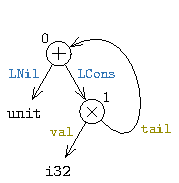
\includegraphics[scale=1.3]{chapters/figures/figTypeTreeList1.pdf}
\end{center}
\vspace{30px}
\caption{\label{fig:typetreelist1}\cons{List} = \cons{LNil} | \newline \cons{LCons}(\type{i32}, \type{List})}
\end{subfigure}%
&
\begin{subfigure}[b]{0.33\textwidth}
\begin{center}
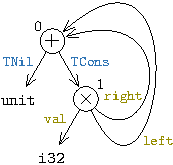
\includegraphics[scale=1.3]{chapters/figures/figTypeTreeTree1.pdf}
\end{center}
\vspace{35px}
\caption{\label{fig:typetreetree1}\cons{Tree} = \cons{TNil} | \newline \cons{TCons}(\type{i32}, \type{Tree}, \type{Tree})}
\end{subfigure}%
&
\begin{subfigure}[b]{0.33\textwidth}
\begin{center}
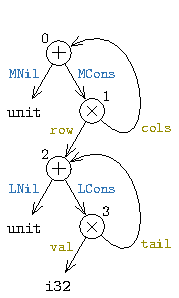
\includegraphics[scale=1.3]{chapters/figures/figTypeTreeMatrix1.pdf}
\end{center}
\caption{\label{fig:typetreematrix1}\cons{Matrix} = \cons{MNil} | \newline \cons{MCons}(\type{List}, \type{Matrix})}
\end{subfigure}%
\\
\end{tabular}
\caption{\label{fig:typetrees}Type trees for the ADTs \type{List}, \type{Tree} and \type{Matrix} respectively.}
\end{figure}

\Cref{fig:typetrees} shows the type trees for three ADTs \type{List}, \type{Tree}, and \type{Matrix} respectively.
In a type tree, each internal node represents either a product (\prodn{}) or a sum (\sumn{}) type constructor.
The leaf nodes are the scalar types.
Each outgoing edge of a \sumn{} node is associated with a data constructor of the corresponding ADT (i.e. \cons{LCons} for \type{List}).
Similarly, each outgoing edge of a \prodn{} node is associated with a field of the corresponding data constructor (i.e. \field{val} for \type{LCons}).
We assign integer indices to the internal nodes and use \ttedge{v}{label}\footnote{
The \ttedge{v}{label} syntax is chosen over $v_1 \rightarrow v_2$ because type trees may have multi-edges, in which case
$v_1 \rightarrow v_2$ no longer represents an unique edge as shown in \cref{fig:typetreetree1}.} to identify the edge outgoing at $v$ associated with {\tt label},
where {\tt label} is either a data constructor or a field name.
The root node is denoted by $v_0$.
The edges going outward from the root node are called {\em tree-edges} e.g., \ttedge{0}{LCons} and \ttedge{1}{val} in \cref{fig:typetreelist1}.
Edges that are not tree-edges, are called {\em back-edges} e.g., \ttedge{1}{cols} in \cref{fig:typetreematrix1}.
Every back-edge induces an unique simple cycle in the type tree representation.

\begin{figure}[H]
\begin{tabular}{@{}c@{}c@{}c@{}}
\begin{subfigure}[b]{0.30\textwidth}
\begin{center}
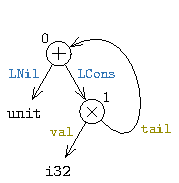
\includegraphics[scale=1.3]{chapters/figures/figTypeTreeList1.pdf}
\end{center}
\vspace{30px}
\caption{\label{fig:typetreelistpeel1} Canonical \type{List} ADT}
\end{subfigure}%
&
\begin{subfigure}[b]{0.33\textwidth}
\begin{center}
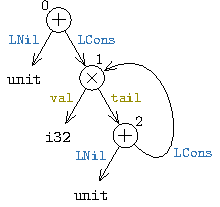
\includegraphics[scale=1.3]{chapters/figures/figTypeTreeList2.pdf}
\end{center}
\vspace{20px}
\caption{\label{fig:typetreelistpeel2} Peeled \type{List} ADT}
\end{subfigure}%
&
\begin{subfigure}[b]{0.33\textwidth}
\begin{center}
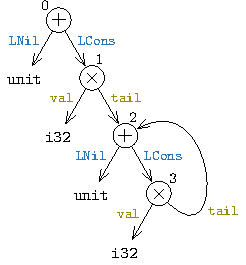
\includegraphics[scale=1.3]{chapters/figures/figTypeTreeList3.pdf}
\end{center}
\caption{\label{fig:typetreelistpeel3} Unrolled \type{List} ADT}
\end{subfigure}%
\\
\end{tabular}
\caption{\label{fig:typetreespeel}Three equivalent graphical representations for \type{List} ADT.
\Cref{fig:typetreelistpeel1} shows the graphical representation of the canonical form of \type{List}.
\Cref{fig:typetreelistpeel2} is obtained by peeling the {\em backedge} [2,1] in \cref{fig:typetreelistpeel1}.
\Cref{fig:typetreelistpeel3} is obtained by unrolling the backedge [2,1] in \cref{fig:typetreelistpeel1} or by
peeling the backedge [4,1] in \cref{fig:typetreelistpeel2} respectively.}
\end{figure}

Recall that types in \SpecL{} (and in IR) follow equirecursive typing rules i.e. types
$\mu \alpha. T$ and $T[\mu \alpha. T/\alpha]$ in \typegrammar{} are {\em equal} types,
where $T[\mu \alpha. T/\alpha]$ represents the new type obtained by substituting all free
instances of $\alpha$ with $\mu \alpha. T$, and is defined as the {\em unfolding} of $\mu \alpha. T$.
In general, under equirecursive typing, two types are equal iff their infinite expansions (through unfolding) are equal.
In the type tree representation, two types are equal iff their infinite expansions are equivalent.
Such type trees are called isomorphic and two types are isomorphic iff they represent the same type.
An unfolding in the term representation corresponds to {\em unrolling} one iteration of a simple cycle in its type tree.
\Cref{fig:typetreespeel} shows three type trees for the \type{List} type.
\Cref{fig:typetreelistpeel1} corresponds to the canonical (intuitively the `smallest') type tree for the \type{List} type.
The type trees \cref{fig:typetreelistpeel2,fig:typetreelistpeel3} are obtained by {\em peeling} and unrolling
the back-edge \ttedge{1}{tail} (in \cref{fig:typetreelistpeel1}) respectively.
Peeling is a form of partial unrolling which only extracts the starting node of the cycle.
In practice, equality of two types (encoded in \typegrammar{}) can be reposed as syntactic
equality of their {\em canonical forms} \cite{canonicalrecursivetypes}.
In general, type trees may contain cycles (due to back-edges) and hence are not quite `trees'.
However, they represent the actual (possibly infinite) trees obtained through repeated unrolling of cycles.

\begin{figure}[H]
\begin{tabular}{cc}
\begin{subfigure}[b]{0.45\textwidth}
\begin{center}
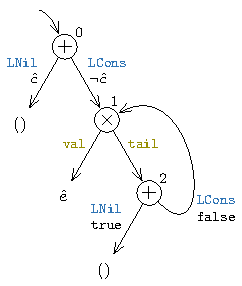
\includegraphics[scale=1.4]{chapters/figures/figValueTreeList1.pdf}
\end{center}
\caption{\label{fig:valuetreelist1}\sumIf{c} \sumThen{\cons{LNil}} \sumElse{\cons{LCons}(e, \cons{LNil})}}
\end{subfigure}%
&
\begin{tabular}{@{}c@{}}
\begin{subfigure}[b]{0.53\textwidth}
\begin{center}
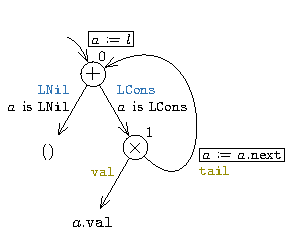
\includegraphics[scale=1.3]{chapters/figures/figValueTreeVarList.pdf}
\end{center}
\caption{\label{fig:valuetreevarlist}$l\ctype{List}$}
\end{subfigure}%
\\
\begin{subfigure}[b]{0.53\textwidth}
\begin{center}
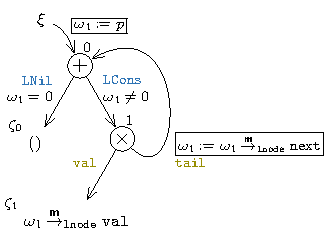
\includegraphics[scale=1.3]{chapters/figures/figValueTreeClist.pdf}
\end{center}
\caption{\label{fig:valuetreeclist}\lifted{list}{\mem{}}{lnode}{p}}
\end{subfigure}%
\\
\end{tabular}
\\
\end{tabular}
\caption{\label{fig:valuetrees}Value trees for three \type{List}-typed expressions.}
\end{figure}

With type trees out of the way, we are ready to present their value analogue called `value trees'.
\Cref{fig:valuetrees} shows the value trees for three \type{List} expressions.
Note that, all three value trees are isomorphic to one of the
\type{List} type trees shown in \cref{fig:typetreespeel}, e.g.,
\cref{fig:valuetreelist2} is isomorphic to \cref{fig:typetreelistpeel2}.
In general, for an expression $e$ of type $\tau$, its value tree $\mathcal{V}(e)$ resembles
its type tree with the following distinctions:

\begin{enumerate}
\item Similar to a type tree, each internal node is either a \sumn{} or a \prodn{} node.
\item Instead of a scalar type $\tau_s$, each leaf node in $\mathcal{V}(e)$ contains an expression
of type $\tau_s$.
\item Similar to the Control-Flow Graph representation (presented in \cref{sec:cfg}), each node $v$
is associated with a symbolic state $\Omega_v$.
\item In addition to a data constructor, each edge originating at a \sumn{} node $v$ also contains
an edge condition expression (a boolean valued function over $\Omega_v$).
We identify such an edge with \vtedge{v}{\mathnormal{V}}{c}, where $v$ is the sum node,
$V$ is a data constructor and $c$ is the edge condition.
The set of edge conditions for all outgoing edges at a \sumn{} node must be mutually exclusive and exhaustive.
\item In addition to a field name, each edge $v \rightarrow v'$ originating at a \prodn{} node $v$ also contains
a transfer function ($\Omega_{v'}$ as a function of $\Omega_v$).
We identify such an edge with \vtedge{v}{fi}{\xfer{}}, where $v$ is the product node,
\field{fi} is a field name and \xfer{} is the transfer function.
\item Additionally, a value tree also contains a special node (called the {\em entry node}), and a special edge
(called the {\em entry edge}) from the entry node to $v_0$ (i.e. the root of the tree).
We use $\xi$ to denote the entry node.
The entry edge is associated with a transfer function $\xfer{}_\xi$.
We often omit the entry node in figures for brevity.
\item A value tree $\mathcal{V}(e)$ can be converted to a type tree $\mathcal{T}$ as follows:
(a) remove the entry node and edge pair, (b) remove edge conditions and transfer functions
associated with all edges, and (c) replace each leaf node expression of (scalar) type $\tau_s$
with $\tau_s$ itself.
The resulting type tree $\mathcal{T}$ represents the type $\tau$ of the expression $e$.
\end{enumerate}

Intuitively, a value tree simultaneously represents the value of the expression as well as
the CFG of its {\em abstracted} deconstruction program.
We will subsequently discuss these properties along with their applications in the context
of our proof discharge algorithm.
Next, we give an algorithm to convert an expression $e$ to its value tree representation $\mathcal{V}(e)$.

\subsection{Conversion of Expressions to their Value Trees}
\label{sec:valuetreeconv}
In this section, we present an algorithm to recursively construct a value tree for any arbitrary expression $e$.
We take a visual approach to align with the graphical nature of value trees.

\begin{figure}[H]
\begin{subfigure}[b]{\textwidth}
\begin{center}
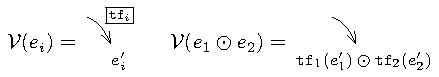
\includegraphics[scale=1.3]{chapters/figures/figValueTreeConvScalar.pdf}
\end{center}
\end{subfigure}
\caption{\label{fig:valuetreeconvscalar} Construction of $\mathcal{V}(e_1 \odot e_2)$ from $\mathcal{V}(e_1)$ and $\mathcal{V}(e_2)$.\\
$\odot$ represents an arbitrary scalar operator.}
\end{figure}

\subsubsection{Scalar Operators}
Given an expression $e = e_1 \odot e_2$,
\cref{fig:valuetreeconvscalar} shows the construction of $\mathcal{V}(e)$
from $\mathcal{V}(e_1)$ and $\mathcal{V}(e_2)$ respectively.
Since $e_1$ and $e_2$ have scalar types, their value trees must have exactly one
node (i.e. the leaf node) containing an expression ($e'_1$ and $e'_2$ respectively) of the same type.
$\odot$ represents an aribtrary scalar operator, i.e. an operator whose arguments
are scalar-typed values (e.g., bitvector arithmatic and relational operators).
Given an expression $s$ and a transfer function \xfer{}, $\xfer{}(s)$
represents the expression obtained by applying \xfer{}, interpreted as a substitution,
to $s$. This is equivalent to the weakest-precondition of $s$ along an edge associated
with the \xfer{}.
The construction shown in \cref{fig:valuetreeconvscalar} can be generalized to
$n$-ary scalar operators for $n>2$.

\begin{figure}[H]
\begin{subfigure}[b]{\textwidth}
\begin{center}
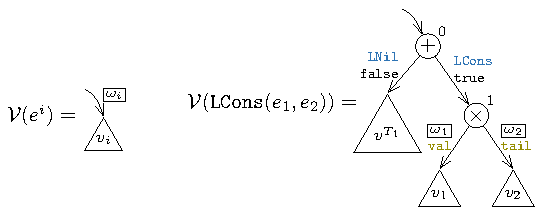
\includegraphics[scale=1.3]{chapters/figures/figValueTreeConvCons.pdf}
\end{center}
\end{subfigure}
\caption{\label{fig:valuetreeconvcons} Construction of $\mathcal{V}(\cons{LCons}(e_1,e_2))$ from $\mathcal{V}(e_1)$ and $\mathcal{V}(e_2)$.\\
$\mathcal{R}_\cons{LNil}$ represents an arbitrary value tree corresponding to the product-type (in \typegrammar{}) associated with \cons{LNil}.}
\end{figure}

\subsubsection{ADT Data Constructors}
Given an expression $e = \cons{LCons}(e_1, e_2)$,
\cref{fig:valuetreeconvcons} depicts the construction of $\mathcal{V}(e)$
from $\mathcal{V}(e_1)$ and $\mathcal{V}(e_2)$ respectively.
In general, for an arbitrary data constructor $V$ of ADT $T$,
the process begins with a \sumn{} node (0 in \cref{fig:valuetreeconvcons})
such that the outgoing edge associated with the value constructor $V$ (\cons{LCons} in \cref{fig:valuetreeconvcons})
has an edge condition of {\tt true} while all other edges are assigned the edge condition {\tt false}.
For each data constructor $V' \neq V$ of $T$, we append a random value tree corresponding to the product-type
associated with $V'$ in \typegrammar{}.
For example, given \type{List} is associated with the sum-type $\mu \alpha. \type{Unit} + (\type{i32} \times \alpha)$,
the product-types associated with \cons{LNil} and \cons{LCons} are:
$\type{Unit}$ and $\mu \alpha. \type{i32} \times (\type{Unit} + \alpha)$ respectively.
We use $\mathcal{R}_\tau$ to denote an arbitrary (i.e. random) value tree of type $\tau$.
For the outgoing edge associated with the data constructor $V$ (\vtedge{0}{LCons}{\tt true} in \cref{fig:valuetreeconvcons}),
we construct a product node (1 in \cref{fig:valuetreeconvcons}) and append the
value trees corresponding to the arguments $e_i$ as children of the product node.
% Interpreted as a program, all random value trees are appended under a {\tt false} edge condition
% (i.e. unreachable) and hence do not change the value represented by $\mathcal{V}(e)$.
% Their only responsibility is to keep the overall structure of $\mathcal{V}(e)$ isomorphic to $\mathcal{T}(\type{List})$.

\begin{figure}[H]
\begin{subfigure}[b]{\textwidth}
\begin{center}
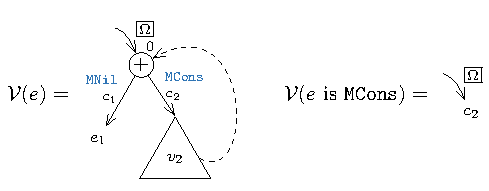
\includegraphics[scale=1.3]{chapters/figures/figValueTreeConvSumIs.pdf}
\end{center}
\end{subfigure}
\caption{\label{fig:valuetreeconvsumis} Construction of $\mathcal{V}(\sumIs{e}{MCons})$ from $\mathcal{V}(e)$.\\
The dashed edge represents the (possibly empty) set of backedges originating in $v_2$ that terminates at 0.}
\end{figure}

\subsubsection{Sum-Is Operator}
Given a {\em sum-is} expression $e' = \sumIs{e}{MCons}$,
\cref{fig:valuetreeconvsumis} shows the construction of $\mathcal{V}(e')$
from $\mathcal{V}(e)$.
The process is rather straightforward and for a general expression $\sumIs{e}{\mathnormal{V}_i}$, entails extracting the
edge condition $c$ ($c_2$ in \cref{fig:valuetreeconvsumis}) from the $\mathcal{V}(\sumIs{e}{\mathnormal{V}_i})$ edge
\vtedge{v_0}{V}{c} (\vtedge{0}{MCons}{c_2} in \cref{fig:valuetreeconvsumis}).
Notice that the entry transfer function $\xfer{}_\xi$ during this conversion.

\begin{figure}[H]
\begin{subfigure}[b]{\textwidth}
\begin{center}
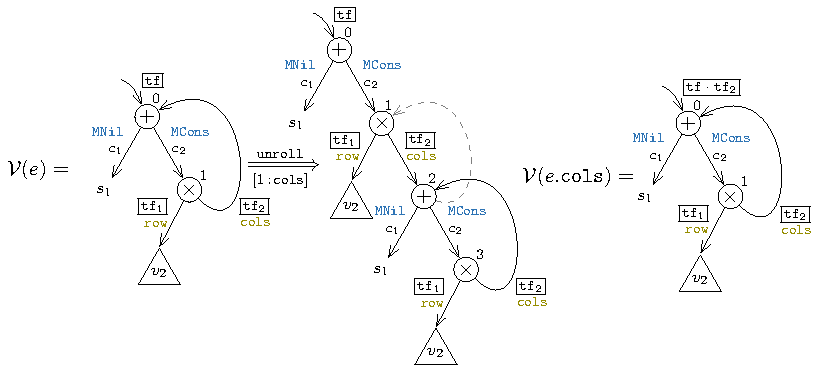
\includegraphics[scale=1.2]{chapters/figures/figValueTreeConvProdAccess.pdf}
\end{center}
\end{subfigure}
\caption{\label{fig:valuetreeconvprodaccess} Construction of $\mathcal{V}(\prodAccess{e}{cols})$ from $\mathcal{V}(e)$.\\
Similar to type trees, {\tt unroll} \ttedge{1}{cols} represents the operation of hoisting one iteration of the cycle \pathset{0,1,0}.}
\end{figure}

\subsubsection{Product-Access Operator}
Given an expression $e' = \prodAccess{e}{cols}$,
\cref{fig:valuetreeconvprodaccess} depicts the construction of $\mathcal{V}(e')$
from $\mathcal{V}(e)$.
Intuitively, $\mathcal{V}(e')$ represents the subtree of $\mathcal{V}(e)$ rooted at the \sumn{} node reached by taking
the edges \vtedge{0}{MCons}{c_2} followed by \vtedge{1}{cols}{\Omega_2}.
However, this path may contain backedges or the subtree itself may contain backedges leaving the subtree.
In such a case, we perform peeling until all such backedges strickly terminate within this subtree.
For example, in \cref{fig:valuetreeconvprodaccess}, the edge \vtedge{1}{cols}{\Omega_2} is a backedge and hence we peel it once.
In the resulting (equivalent) value tree, the subtree (rooted at 2) contains a backedge leaving the subtree which requires
one more peeling operation.
The resulting value tree contains the subtree rooted at the \sumn{} node 2 which satisfies the two conditions above and
hence $\mathcal{V}(e')$ is simply constructed by extracting the subtree rooted at \sumn{} node 2.
Note that we preserve the transfer functions from the entry to the \sumn{} node 2 during extraction.
$\xfer{}_1 \cdot \xfer{}_2$ represents the composition of the transfer functions $\xfer{}_1$ and $\xfer{}_2$ respectively.

\begin{figure}[H]
\begin{subfigure}[b]{\textwidth}
\begin{center}
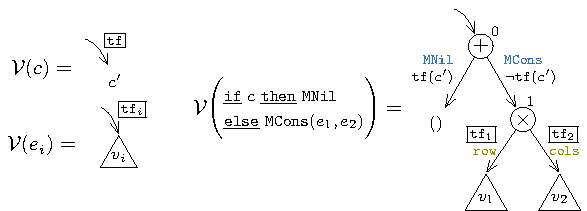
\includegraphics[scale=1.3]{chapters/figures/figValueTreeConvIte.pdf}
\end{center}
\end{subfigure}
\caption{\label{fig:valuetreeconvite} Construction of $\mathcal{V}($ \sumIf{c} \sumThen{\cons{MNil}} \sumElse{\cons{MCons}(e_1,e_2)} $)$ from $\mathcal{V}(c)$, $\mathcal{V}(e_1)$ and $\mathcal{V}(e_2)$.}
\end{figure}

\subsubsection{\underline{If}-\underline{Then}-\underline{Else} Operator}
Given an expression $e =$ \sumIf{c} \sumThen{\cons{MNil}} \sumElse{\cons{MCons}(e_1,e_2)},
\cref{fig:valuetreeconvite} describes the construction of $\mathcal{V}(e)$
using $\mathcal{V}(c)$, $\mathcal{V}(e_1)$ and $\mathcal{V}(e_2)$.
Let us consider a general \sumDtor{} expression $e$ (associated with the ADT $T$ with data constructors $V_1,V_2,\dots,V_n$)
such that the branch associated with $V_i$ is given by $V_i(e_i^1,e_i^2,\dots)$.
We begin with the construction of a \sumn{} root node (0 in \cref{fig:valuetreeconvite})
such that the outgoing edge associated with $V_i$ has the edge condition equal to the
expression path condition of the branch $V_i(e_i^1,e_i^2,\dots)$
($\xfer{}(c')$ and $\neg \xfer{}(c')$ for \cons{MNil} and \cons{MCons} respectively in \cref{fig:valuetreeconvite}).
For each outgoing edge associated with the data constructor $V_i$, we construct a \prodn{} node
(1 for \cons{MCons} in \cref{fig:valuetreeconvite}) and append the value trees corresponding to
the arguments $e_i^j$ as its children.

\begin{figure}[H]
\begin{subfigure}[b]{\textwidth}
\begin{center}
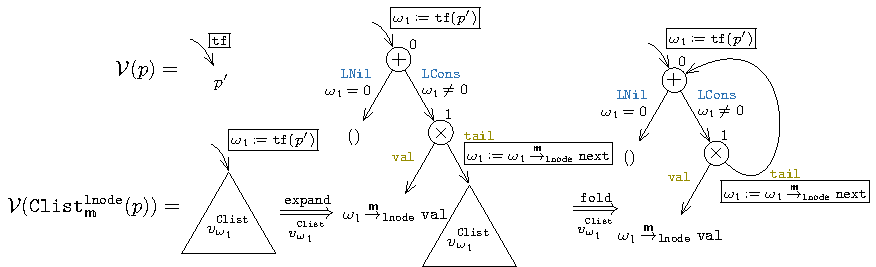
\includegraphics[scale=1.2]{chapters/figures/figValueTreeConvLift.pdf}
\end{center}
\end{subfigure}
\caption{\label{fig:valuetreeconvlift} Construction of $\mathcal{V}(\lifted{list}{\mem{}}{lnode}{p})$ from $\mathcal{V}(p)$.\\
The process involves assuming $v_\vtse{1}^\lift{list}{}{}$ to be the value tree of $\lifted{list}{\mem{}}{lnode}{\vtse{1}}$,
followed by expansion of $v_\vtse{1}^\lift{list}{}{}$ using the definition of \lift{list}{\mem{}}{lnode} (in \cref{eqn:clist})
and, finally folding the tree-edge \ttedge{1}{tail} incident on the self-referencial subtree $v_\vtse{1}^\lift{list}{}{}$ into a backedge.}
\end{figure}

\subsubsection{Lifting Constructor}
Given an expression $e = \lifted{list}{\mem{}}{lnode}{p}$,
\cref{fig:valuetreeconvlift} shows the construction of $\mathcal{V}(e)$
from $\mathcal{V}(p)$.
Recall the recursive definition of the lifting constructor \lift{list}{\mem{}}{lnode} given in
\cref{eqn:clist}.
We start by assuming that $v_\vtse{1}^\lift{list}{}{}$ is the value tree for the lifted expression
\lifted{list}{\mem{}}{lnode}{\vtse{1}}.
Hence, the value tree of \lifted{list}{\mem{}}{lnode}{p} is identical to $v_\vtse{1}^\lift{list}{}{}$
except we assign the actual argument (i.e. $\xfer{}(p')$) to the formal argument $\vtse{1}$ along the
entry edge.
Next, we expand the subtree $v_\vtse{1}^\lift{list}{}{}$ based on the unrolling procedure of \lift{list}{\mem{}}{lnode}
(defined in \cref{eqn:clist}) until the entire value tree becomes a self-referencial structure.
For example, after expanding through \cref{eqn:clist} once in \cref{fig:valuetreeconvlift},
the value tree contains an tree-edge \ttedge{1}{tail} incident on the self-referencial subtree $v_\vtse{1}^\lift{list}{}{}$.
In the last step, we fold all self-referencial tree-edges (\ttedge{1}{tail} in \cref{fig:valuetreeconvlift})
by converting them into backedges terminating at the root of the subtree being referenced
(0 for $v_\vtse{1}^\lift{list}{}{}$ in \cref{fig:valuetreeconvlift}).

\begin{figure}[H]
\begin{subfigure}[b]{\textwidth}
\begin{center}
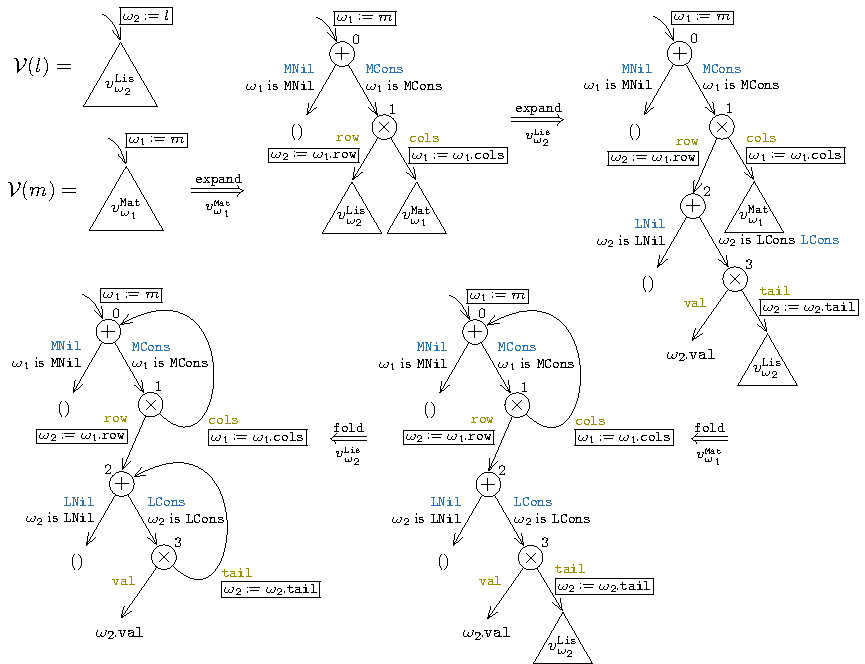
\includegraphics[scale=1.2]{chapters/figures/figValueTreeConvVar.pdf}
\end{center}
\end{subfigure}
\caption{\label{fig:valuetreeconvvar} Construction of $\mathcal{V}(m)$ for a \type{Matrix} variable $m$.
The process is identical to the construction of value trees for lifted expressions as shown in \cref{fig:valuetreeconvlift}.}
\end{figure}

\subsubsection{Variables}
Finally, we are interested in constructing the value tree for a variable.
Recall that, every ADT (pseudo-)variable is associated with an unrolling procedure
characterized by the ADT itself. e.g. \cref{eqn:specDeconstruct}
for the \type{List} variable $l$.
The \type{Matrix} ADT is defined as:
$\type{Matrix} = \cons{MNil} \ | \ \cons{MCons}(\type{List},\type{Matrix})$,
and thus the unrolling procedure for a \type{Matrix} variable $m$ is given by:

\begin{equation}
\label{matrixunrollingprocedure}
m = \sumIf{\sumIs{m}{MNil}} \  \sumThen{\cons{MNil}} \  \sumElse{\cons{MCons}(\prodAccess{m}{row}, \prodAccess{m}{cols})}
\end{equation}

\Cref{fig:valuetreeconvvar} illustrates the construction $\mathcal{V}(m)$ for the \type{Matrix} variable $m$.
The process consists of the same three steps used to construct the value tree
for a lifted expression -- assume, expand and fold.
First, we assume that $v_\vtse{1}^\type{Mat}$ and $v_\vtse{2}^\type{Lis}$ are the value trees
corresponding to the pseudo-variables \vtse{1} and \vtse{2} of \type{Matrix} and \type{List}
types respectively.
Thus, $\mathcal{V}(m)$ is equal to $v_\vtse{1}^\type{Mat}$ with the entry edge transfer function
$\{ \vtse{1} \mapsfrom m \}$.
We expand the definitions of $v_\vtse{1}^\type{Mat}$ and $v_\vtse{2}^\type{Lis}$ once each before
the value tree becomes self-referencial.
Finally, we fold the treeedges \ttedge{1}{cols} and \ttedge{3}{tail} into the back-edges
terminating at the roots of the subtrees representing $v_\vtse{1}^\type{Mat}$ and $v_\vtse{2}^\type{Lis}$
respectively (nodes 0 and 3 in \cref{fig:valuetreeconvvar}).

\subsection{Applications of Value Trees}
\label{sec:valuetreeapps}
With the conversion algorithm out of the way, we next discuss a handful of properties of value trees along with
their applications, in the context of our proof discharge algorithm.

\subsubsection{Program Interpretation of Value Trees}
\label{sec:valuetreeasprog}
A value tree $\mathcal{V}$ can be interpreted as a {\em non-deterministic} Control-Flow Graph corresponding to a program.
Similar to the CFG representation, every node $v$ is associated with a symbolic state $\Omega_n$.
In this interpretation, edges without an edge condition (e.g., outgoing at a \prodn{} node) are assigned the {\tt true}
edge condition. Similarly, edges without a transfer function (e.g., outgoing at a \sumn{} node) are assigned an
identity transfer function.
The entry node $\xi$ is the start node and each leaf node $\zeta$ represents an exit node.
An edge incident on a leaf node $\zeta$ (containing an expression $e$) is called an exit edge and is associated
with an observable action that returns $e$.

\begin{figure}[t!]
\begin{tabular}{@{\hskip 2mm}c@{}c@{}}
\begin{subfigure}[b]{0.5\textwidth}
\begin{center}
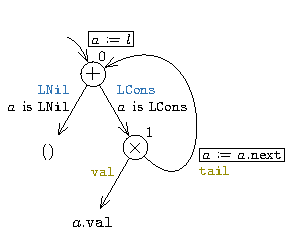
\includegraphics[scale=1.35]{chapters/figures/figValueTreeVarList.pdf}
\end{center}
\vspace{4px}
\caption{\label{fig:valuetreevar}$\mathcal{V}(l)$}
\end{subfigure}%
&
\begin{subfigure}[b]{0.5\textwidth}
\begin{center}
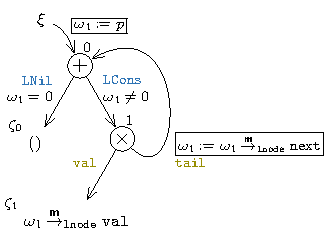
\includegraphics[scale=1.35]{chapters/figures/figValueTreeClist.pdf}
\end{center}
\caption{\label{fig:valuetreelifted}$\mathcal{V}(\lifted{list}{\mem{}}{lnode}{p})$}
\end{subfigure}%
\\
\end{tabular}
\caption{\label{fig:valuetreeapproxeg}Value trees for a \type{List} variable $l$ and a lifted expression \lifted{list}{\mem{}}{lnode}{p} respectively.}
\end{figure}

\subsubsection{Canonical Deconstruction Property}
\label{sec:valuetreecanonicaldecons}
A path originating at the entry node $\xi$ and terminating at an exit node $\zeta$ is called an
{\em execution path} and is denoted by $\execpath{}$.
Generalizing the edge syntax, $\ttedge{v}{label_1,label_2,\dots ,label_n}$ represents the path
starting at $v$ such that its $n$ consecutive edges are associated with the labels ${\tt label}_i \forall i \in [1,n]$.
Hence, an execution path \execpath{} can be written as $\xi \rightarrow \ttedge{v_0}{label_1,label_2,\dots ,label_n}$,
or $\execpath{}[{\tt label_1,label_2,\dots,label_n}]$ in short.
Recall that, edges leaving a \prodn{} node are associated with field names.
The {\em field trace of \execpath{}}, $\ftrace{\execpath{}}$ is defiend as the ordered list of field names associated with edges in the path \execpath{}.
For an execution path $\execpath{}[\cons{LCons},\field{tail},\cons{LCons},\field{val}]$ in the value tree shown in \cref{fig:valuetreevar},
$\ftrace{\execpath{}}$ is given by $[\field{tail},\field{val}]$.
Given a value tree $\mathcal{V}(e)$ and an execution path $\execpath{}$ with a field trace $[{\tt a_1,a_2,\dots,a_n}]$,
$\prodAccess{e}{a_1,a_2,.,a_n}$ is defined as the component of $e$ with respect to $\execpath{}$, denoted by $\comp{e}{\execpath{}}$.
The {\em canonical deconstruction property} for a value tree ensures that:

\begin{enumerate}
\item The condition under which $\comp{e}{\execpath{}}$ is accessible (i.e. is well-formed as discussed in \cref{sec:irconv})
is equal to the path condition of $\execpath{}$, denoted by $\pathcond{\execpath{}}$.
\item The value of $\comp{e}{\execpath{}}$ is equal to the value returned by $\mathcal{V}(e)$ (interpreted as a program) along the
execution path $\execpath{}$. This is equivalent to the weakest-precondition of the value returned along the path $\execpath{}$
and is denoted by $\retval{\execpath{}}$.
\item Both $\pathcond{\execpath{}}$ and $\retval{\execpath{}}$ are in the canonical form (\cref{sec:canonicalalgo}).
\end{enumerate}

Consider the value tree corresponding to the lifted expression $e=\lifted{list}{\mem{}}{lnode}{p}$ as shown in \cref{fig:valuetreelifted}.
The execution path $\execpath{}[\cons{LCons},\field{val}]$ corresponds to the component $\comp{e}{\execpath{}} = \prodAccess{\lifted{list}{\mem{}}{lnode}{p}}{val}$.
The path condition and the value returned along $\execpath{}$ are given by $\pathcond{\execpath{}} = (p \neq 0)$ and
$\retval{\execpath{}} = \structPointer{p}{\mem{}}{lnode}{val}$ respectively.
Note that $\comp{e}{\execpath{}}$ is well-formed iff $\pathcond{\execpath{}}$ is true and
$\comp{e}{\execpath{}} = \retval{\execpath{}}$.
Furthermore, both are in canonical forms.

\subsubsection{Reduction of Approximate Recursive Relations}
\label{sec:valuetreeapprox}
Since an ADT represents a `sum of product' type, each level of an ADT value
(in its expression tree as shown in \cref{sec:adtdepth}) corresponds to two levels -- \sumn{} and \prodn{}
in the value tree representation.
Combining the above observation with the value tree properties discussed above (\cref{sec:valuetreeasprog,sec:valuetreecanonicaldecons})
allow us reformulate approximate \recursiveRelations{} between $l_1$ and $l_2$ as {\em bounded} equivalence \cite{boundedmodelchecking}
between $\mathcal{V}(l_1)$ and $\mathcal{V}(l_2)$.
The $d$-depth over-approximation $l_1 \indEqDepth{d} l_2$ asserts that $\mathcal{V}(l_1)$ and $\mathcal{V}(l_2)$ are equivalent
for all execution paths up to a depth\footnote{
The depth of an execution path \execpath{} is defined as the depth of the exit node in the unrolled (executable) value tree.
If \execpath{} contains $n$ edges (including the entry edge), then its depth is equal to $(n-1)$.} of $2 \cdot d$ .
Clearly, this is a weaker condition because $\mathcal{V}(l_1)$ and $\mathcal{V}(l_2)$ may behave differently for longer execution paths.
The $d$-depth under-approximation $l_1 \indEqUapprox{d} l_2$ asserts that $\mathcal{V}(l_1)$ and $\mathcal{V}(l_2)$ are equivalent for
all execution paths up to a depth of $2 \cdot d$ and all other execution paths are unreachable.
This is a stronger condition than general equivalence because paths deeper than $2 \cdot d$ may indeed be reachable.
Let $\execpaths{\delta}{l_1}{l_2}$ be the set of all execution path pairs $\langle \execpath{}_1, \execpath{}_2 \rangle$
such that $\ftrace{\execpath{}_1} = \ftrace{\execpath{}_2}$ and depth of $\execpath{}_1$ and $\execpath{}_2$ is $\delta$.
For example, consider the value trees shown in \cref{fig:valuetreeapproxeg} corresponding to the \type{List} values
$e_1 = l$ and $e_2 = \lifted{list}{\mem{}}{clnode}{p}$ respectively.
Then, $\execpaths{0}{e_1}{e_2} = \emptyset$, $\execpaths{1}{e_1}{e_2} = \{ \langle \pathset{\xi,0,\zeta_0},\pathset{\xi,0,\zeta_0} \rangle \}$
and $\execpaths{2}{e_1}{e_2} = \{ \langle \pathset{\xi,0,1,\zeta_1},\pathset{\xi,0,1,\zeta_1} \rangle \}$.
Finally, the $d$-depth approximations of $l_1 \indEq{} l_2$ are given by:

\begin{equation}
\label{eqn:valuetreeapprox}
\begin{footnotesize}
\begin{aligned}
l_1 \indEqDepth{d} l_2 &= \sum_{\delta=0}^{2 \cdot d} \Bigg( \bigwedge_{\substack{\langle \execpath{}_1, \execpath{}_2 \rangle \\ \in \execpaths{\delta}{l_1}{l_2}}} \begin{array}{@{}c@{}} \pathcond{\execpath{}_1} = \pathcond{\execpath{}} \\ \retval{\execpath{}_1} = \retval{\execpath{}_2} \end{array} \Bigg) \\
l_1 \indEqUapprox{d} l_2 &= \sum_{\delta=0}^{2 \cdot d} \Bigg( \bigwedge_{\substack{\langle \execpath{}_1, \execpath{}_2 \rangle \\ \in \execpaths{\delta}{l_1}{l_2}}} \begin{array}{@{}c@{}} \pathcond{\execpath{}_1} = \pathcond{\execpath{}} \\ \retval{\execpath{}_1} = \retval{\execpath{}_2} \end{array} \Bigg) \land \Bigg( \bigwedge_{\substack{\langle \execpath{}_1, \execpath{}_2 \rangle \\ \in \execpaths{2 \cdot d + 1}{l_1}{l_2}}} \begin{array}{@{}c@{}} \neg \pathcond{\execpath{}_1} \\ \neg \pathcond{\execpath{}_2} \end{array} \Bigg)
\end{aligned}
\end{footnotesize}
\end{equation}

Recall that the canonical deconstruction property ensures that the reductions in \cref{eqn:valuetreeapprox} are in the canonical form.
The value trees $\mathcal{V}(l_1 \indEqDepth{d} l_2)$ and $\mathcal{V}(l_1 \indEqUapprox{d} l_2)$ contains a single (leaf) node with the boolean
expressions given in \cref{eqn:valuetreeapprox}.
The conversion algorithm presented in \cref{sec:valuetreeconv} together with the handling of approximate \recursiveRelations{} described above
enables the reduction of a proof obligation $P$ without \recursiveRelations{} directly to its canonical form by --
(a) constructing $\mathcal{V}(P)$ and (b) extracting the boolean expression at its root.

\subsubsection{Bisimilarity of Value Trees}
\label{sec:valuetreebisim}
Unlike its approximations, a \recursiveRelation{} $l_1 \indEq{} l_2$ asserts complete equivalence between
$\mathcal{V}(l_1)$ and $\mathcal{V}(l_2)$ respectively.
Similar to our top-level equivalence check between \sprog{} and \cprog{},
we attempt to prove that $\mathcal{V}(l_1)$ and $\mathcal{V}(l_2)$ are bisimilar.
To make the search for a bisimulation relation easier, we peel $\mathcal{V}(l_1)$ and $\mathcal{V}(l_2)$
to unify their static structures.
Once unified, the bisimulation relation requires the inference of inductive invariants at correlated nodes such that
under the precondition at $(\xi\!:\!\xi)$, inductive invariants hold and both $\mathcal{V}(l_1)$ and $\mathcal{V}(l_2)$
have equal observables at correlated exit nodes $(\zeta_i\!:\!\zeta_i)$.

\begin{figure}[t!]
\begin{tabular}{@{}c@{}}
\begin{subfigure}[b]{0.5\textwidth}
\begin{center}
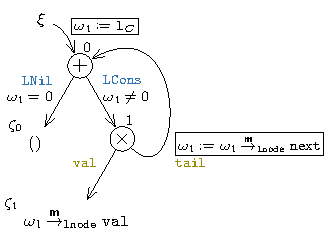
\includegraphics[scale=1.25]{chapters/figures/figValueTreeClistm.pdf}
\end{center}
\caption{\label{fig:valuetreeclistm}$\mathcal{V}(\lifted{list}{\mem{}}{lnode}{\cv{l}})$}
\end{subfigure}%
\begin{subfigure}[b]{0.5\textwidth}
\begin{center}
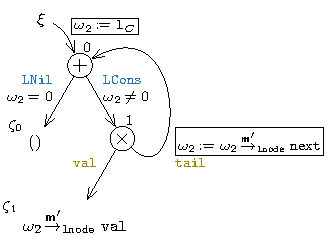
\includegraphics[scale=1.25]{chapters/figures/figValueTreeClistmdash.pdf}
\end{center}
\caption{\label{fig:valuetreeclistmdash}$\mathcal{V}(\lifted{list}{\mem{}'}{lnode}{\cv{l}})$}
\end{subfigure}%
\\
\begin{subfigure}[b]{\textwidth}
\begin{center}
\begin{footnotesize}
\begin{tabular}{@{\hskip 5mm}cl@{\hskip 8mm}l@{\hskip 8mm}l@{\hskip 3mm}}
\toprule
{\bf Node Pair} & \multicolumn{3}{c}{\bf Invariants} \\
\toprule
$(\xi \!:\! \xi)$ & \multicolumn{3}{l}{$\circled{\small P} \  \lhs{}$ in \cref{eqn:cat3revisit}} \\
\midrule
\multirow{3}{*}{\makecell[c]{$(0 \!:\! 0)$ \\ $(1 \!:\! 1)$ }} & $\circled{\footnotesize I1} \  \vtse{1} = \vtse{2}$ & $\circled{\footnotesize I2} \  \vtse{1} \pointsTo{} \{ \mlrs{\cpc{4}}, \heapr \}$ & $\circled{\footnotesize I3} \  \vtse{2} \pointsTo{} \{ \mlrs{\cpc{4}}, \heapr \}$ \\
& $\circled{\footnotesize I4} \ \cv{p} \pointsTo{} \{ \mlrs{\cpc{4}} \}$ & $\circled{\footnotesize I5} \  \cv{l} \pointsTo{} \{ \mlrs{\cpc{4}} \}$ \\
& $\circled{\footnotesize I6} \ \mlrf{\cpc{4}} \pointsTo{} \{ \mlrs{\cpc{4}} \}$ & $\circled{\footnotesize I7} \  \mlrs{\cpc{4}} \pointsTo{} \{ \mlrs{\cpc{4}}, \heapr{} \}$ & $\circled{\footnotesize I8} \ \heapr{} \pointsTo{} \{ \mlrs{\cpc{4}}, \heapr{} \}$ \\
\midrule
$(\zeta_0 \!:\! \zeta_0)$ & \multicolumn{3}{l}{$\circled{\scriptsize E1} \  () = ()$} \\
\midrule
$(\zeta_1 \!:\! \zeta_1)$ & \multicolumn{3}{l}{$\circled{\scriptsize E2} \  \structPointer{\vtse{1}}{\mem{}}{lnode}{val} = \structPointer{\vtse{2}}{\mem{}'}{lnode}{val}$} \\
\bottomrule
\end{tabular}
\end{footnotesize}
\end{center}
\caption{\label{fig:valuetreeinvs}Invariants table for bisimulation relation between \cref{fig:valuetreeclistm} and \cref{fig:valuetreeclistmdash}.}
\end{subfigure}
\end{tabular}
\caption{\label{fig:valuetreebisim}Value trees of \lifted{list}{\mem{}}{lnode}{\cv{l}} and \lifted{list}{\mem{}'}{lnode}{\cv{l}} along with
their associated node invariants at correlated node pairs.}
\vspace{-10px}
\end{figure}

Recall the type III proof obligation illustrated in \cref{sec:cat3}:
\begin{equation}
\label{eqn:cat3revisit}
\lhs{} \Rightarrow \lifted{list}{\mem{}}{lnode}{\cv{l}} \indEq{} \lifted{list}{\mem{}'}{lnode}{\cv{l}}
\end{equation}
Also recall the points-to invariants available at \cpc{5} (showing only the relevant ones):
$\cv{p} \pointsTo{} \{ \mlrf{\cpc{4}} \}$
$\cv{l} \pointsTo{} \{ \mlrs{\cpc{4}} \}$, $\mlrf{\cpc{4}} \pointsTo{} \{ \mlrs{\cpc{4}} \}$,
$\mlrs{\cpc{4}} \pointsTo{} \{ \mlrs{\cpc{4}}, \heapr{} \}$, and
$\heapr{} \pointsTo{} \{ \mlrs{\cpc{4}}, \heapr{} \}$.
Similar to a deconstruction program, we run our points-to analysis on the value trees to identify
potentially beneficial points-to invariants at all correlated nodes.
\Cref{fig:valuetreebisim} shows the value trees of $\lifted{list}{\mem{}}{lnode}{\cv{l}}$
and $\lifted{list}{\mem{}'}{lnode}{\cv{l}}$ along with the table of invariants
required for a successful bisimulation check.

\section{Evaluation}
\label{sec:eval}

We have implemented \toolName{} on top of the Counter tool \cite{oopsla20}.
We use {\em four} SMT solvers running in parallel for solving
SMT proof obligations discharged by our proof discharge algorithm:
{\tt z3-4.8.7}, {\tt z3-4.8.14} \cite{z3}, {\tt Yices2-45e38fc} \cite{yices}, and {\tt cvc4-1.7} \cite{cvc4solver}.
An unroll factor of {\em four} is used to handle loop unrolling in the C implementation.
We use a default value of {\em eight} for over- and under-approximation depths ($d_o$ and $d_u$).
The default value of our unrolling parameter $k$ (used for categorization of proof obligations) is {\em five}.
We use a value of {\em five} for $\eta$ (used by {\em StrongestInvCover()} during weakening of \recursiveRelation{} invariants).

\toolName{} requires the user to provide a \SpecL{} program $S$ (specification), a C implementation $C$,
and a file that contains their input-output specifications.
An equivalence check requires the identification of lifting constructors to relate C
values to the ADT values in \SpecL{} through  \recursiveRelations{}.
Such relations may be required at the entry of both programs (i.e. in the precondition $Pre$),
in the middle of both programs (i.e., in the invariants at intermediate product-CFG nodes),
and at the exit of both programs (i.e., in the postcondition $Post$).
$Pre$ and $Post$ are user-specified, whereas the inductive invariants are
inferred automatically by our algorithm.
During invariant inference, \toolName{} derives the candidate lifting constructors
from the user-specified $Pre$ and $Post$.
More sophisticated approaches to finding lifting constructors are left as future work.

\subsection{Experiments}
We consider programs involving four distinct ADTs, namely,
\inv{\small T1} \type{String}, \inv{\small T2} \type{List}, \inv{\small T3} \type{Tree}
and \inv{\small T4} \type{Matrix}.
For each \SpecL{} program specification, we consider multiple
C implementations that differ in their (a) layout and representation of ADTs, and
(b) algorithmic strategies. For example, a \type{Matrix}, in C, may be laid out
in a two-dimensional array, a one-dimensional array using row or column major
layouts etc. On the other hand, an optimized implementation may choose manual vectorization
of an inner-most loop. Next, we consider each ADT in more detail. For each,
we discuss (a) its corresponding programs, (b) C memory layouts and their lifting
constructors, and (c) varying algorithmic strategies.

\begin{table}[t]
\caption{\label{tab:LiftingConsStr}String lifting constructors and their definitions.}
\vspace{-5px}
\begin{scriptsize}
\begin{center}
\begin{tabular}{|l|l|}
\hline
\multicolumn{1}{|c|}{\Tstrut \Bstrut\footnotesize Lifting Constructor} & \multicolumn{1}{c|}{\Tstrut \Bstrut \footnotesize Definition} \\
\hline
\hline
% \multicolumn{2}{|c|}{\Tstrut \Bstrut \inv{T1} {\tt List = LNil | LCons(i32, List)}} \\
% \hline
% $\mathrm{Clist^{u32[]}_m(p\ i\ n : i32)}$ & \makecell[l]{\Tstrut $\mathrm{\underline{if}\ (i\geq_{u}n)}$ $\mathrm{\underline{then}\ LNil}$ \\ \Bstrut $\mathrm{\underline{else}\ LCons(p[i]^m_{i32}, Clist^{u32[]}_m(p,i+1_{i32},n))}$} \\
% \hline
% $\mathrm{Clist^{lnode(u32)}_m(p:i32)}$ & \makecell[l]{\Tstrut $\mathrm{\underline{if}\ (p==0_{i32})}$ $\mathrm{\underline{then}\ LNil}$ \\ \Bstrut $\mathrm{\underline{else}\ LCons(\structPointer{\tt p}{m}{\tt lnode}{val}, Clist^{lnode}_m(\structPointer{\tt p}{m}{\tt lnode}{next})}$} \\
% \hline
% $\mathrm{Clist^{clnode(u32)}_m(p:i32,i:i2)}$ & \makecell[l]{\Tstrut $\mathrm{\underline{if}\ (p==0_{i32})}$ $\mathrm{\underline{then}\ LNil}$ \\ \Bstrut $\mathrm{\underline{else}\ LCons(\structPointer{\tt p}{m}{\tt clnode}{chunk}[i]^m_{i32}, Clist^{clnode}_m((ite(i==3_{i2}, \structPointer{\tt p}{m}{\tt clnode}{next},p), i+1_{i2}))}$} \\
% \hline
% $\mathrm{Clist^{u32[r]}_m(p\ i\ j\ u\ v:i32)}$ & \makecell[l]{\Tstrut $\mathrm{\underline{if}\ (j\geq_{u}v)}$ $\mathrm{\underline{then}\ LNil}$ \\ \Bstrut $\mathrm{\underline{else}\ LCons(p[i*v+j]^m_{i32}, Clist^{u32[r]}_m(p,i,j+1_{i32},u,v))}$} \\
% \hline
% $\mathrm{Clist^{u32[c]}_m(p\ i\ j\ u\ v:i32)}$ & \makecell[l]{\Tstrut $\mathrm{\underline{if}\ (j\geq_{u}v)}$ $\mathrm{\underline{then}\ LNil}$ \\ \Bstrut $\mathrm{\underline{else}\ LCons(p[i+j*u]^m_{i32}, Clist^{u32[c]}_m(p,i,j+1_{i32},u,v))}$} \\
% \hline
% \hline
% \multicolumn{2}{|c|}{\Tstrut \Bstrut \inv{T2} {\tt Tree = TNil | TCons(i32, Tree, Tree)}} \\
% \hline
% $\mathrm{Ctree^{u32[]}_m(p\ i\ n : i32)}$ & \makecell[l]{\Tstrut $\mathrm{\underline{if}\ (i \geq_{u} n)}$ $\mathrm{\underline{then}\ TNil}$ \\ \Bstrut $\mathrm{\underline{else}\ TCons(p[i]^{i32}_m, Ctree^{u32[]}_m(p,2_{i32}*i+1_{i32},n), Ctree^{u32[]}_m(p,2_{i32}*i+2_{i32},n))}$ } \\
% \hline
% $\mathrm{Ctree^{tnode(u32)}_m(p:i32)}$ & \makecell[l]{\Tstrut $\mathrm{\underline{if}\ (p==0_{i32})}$ $\mathrm{\underline{then}\ TNil}$ \\ \Bstrut $\mathrm{\underline{else}\ TCons(\structPointer{\tt p}{m}{\tt tnode}{val}, Ctree^{tnode}_m(\structPointer{\tt p}{m}{\tt tnode}{left}), Ctree^{tnode}_m(\structPointer{\tt p}{m}{\tt tnode}{right}))}$ } \\
% \hline
% \hline
\multicolumn{2}{|c|}{\Tstrut \Bstrut \inv{T1} {\tt Str = SInvalid | SNil | SCons(i8, Str)}} \\
\hline
$\mathrm{Cstr^{u8[]}_m(p:i32)}$ & \makecell[l]{\Tstrut $\mathrm{\underline{if}\ (p==0_{i32})}$ $\mathrm{\underline{then}\ SInvalid}$ \\ \Tstrut $\mathrm{\underline{else\ if}\ (p[0_{i32}]^m_{i8}==0_{i8})\ \underline{then}\ SNil}$ \\ \Bstrut $\mathrm{\underline{else}\ SCons(p[0_{i32}]^m_{i8}, Cstr^{u8[]}_m(p+1_{i32}))}$} \\
\hline
$\mathrm{Cstr^{lnode(u8)}_m(p:i32)}$ & \makecell[l]{\Tstrut $\mathrm{\underline{if}\ (p==0_{i32})}$ $\mathrm{\underline{then}\ SInvalid}$ \\ \Tstrut $\mathrm{\underline{else\ if}\ (\structPointer{\tt p}{m}{\tt lnode}{val} == 0_{i8})\ \underline{then}\ SNil}$ \\ \Bstrut $\mathrm{\underline{else}\ SCons(\structPointer{\tt p}{m}{\tt lnode}{val}, Cstr^{lnode(u8)}_m(\structPointer{\tt p}{m}{\tt lnode}{next}))}$} \\
\hline
$\mathrm{Cstr^{clnode(u8)}_m(p:i32,i:i2)}$ & \makecell[l]{\Tstrut $\mathrm{\underline{if}\ (p==0_{i32})}$ $\mathrm{\underline{then}\ SInvalid}$ \\ \Tstrut $\mathrm{\underline{else\ if}\ (\structPointer{\tt p}{m}{\tt clnode}{chunk} [i]^m_{i8} == 0_{i8})\ \underline{then}\ SNil}$ \\ \Bstrut $\mathrm{\underline{else}\ SCons(\structPointer{\tt p}{m}{\tt clnode}{chunk} [i]^m_{i8},}$ \\ \qquad \qquad \quad $\mathrm{Cstr^{clnode(u8)}_m((i==3_{i2}\ ?\ \structPointer{\tt p}{m}{\tt clnode}{next}\ :\ p), i+1_{i2}))}$} \\
\hline
% \hline
% \multicolumn{2}{|c|}{\Tstrut \Bstrut \inv{T4} {\tt Matrix = MNil | MCons(List, Matrix)}} \\
% \hline
% $\mathrm{Cmat^{u32[][]}_m(p\ i\ u\ v:i32)}$ & \makecell[l]{\Tstrut $\mathrm{\underline{if}\ (i \geq_{u} u)}$ $\mathrm{\underline{then}\ MNil}$ \\ \Bstrut $\mathrm{\underline{else}\ MCons(Clist^{u32[]}_m(p[i]^m_{i32},0_{i32},v), Cmat^{u32[][]}_m(p,i+1_{i32},u,v))}$} \\
% \hline
% $\mathrm{Cmat^{u32[r]}_m(p\ i\ u\ v:i32)}$ & \makecell[l]{\Tstrut $\mathrm{\underline{if}\ (i \geq_{u} u)}$ $\mathrm{\underline{then}\ MNil}$ \\ \Bstrut $\mathrm{\underline{else}\ MCons(Clist^{u32[r]}_m(p,i,0_{i32},u,v), Cmat^{u32[r]}_m(p,i+1_{i32},u,v))}$} \\
% \hline
% $\mathrm{Cmat^{u32[c]}_m(p\ i\ u\ v:i32)}$ & \makecell[l]{\Tstrut $\mathrm{\underline{if}\ (i \geq_{u} u)}$ $\mathrm{\underline{then}\ MNil}$ \\ \Bstrut $\mathrm{\underline{else}\ MCons(Clist^{u32[c]}_m(p,i,0_{i32},u,v), Cmat^{u32[c]}_m(p,i+1_{i32},u,v))}$} \\
% \hline
% $\mathrm{Cmat^{lnode(u32[])}_m(p\ v:i32)}$ & \makecell[l]{\Tstrut $\mathrm{\underline{if}\ (p==0_{i32})}$ $\mathrm{\underline{then}\ MNil}$ \\ \Bstrut $\mathrm{\underline{else}\ MCons(Clist^{u32[]}_m(\structPointer{\tt p}{m}{\tt lnode}{val},0_{i32},v),Cmat^{lnode(u32[])}_m(\structPointer{\tt p}{m}{\tt lnode}{next},v))}$} \\
% \hline
% $\mathrm{Cmat^{lnode(u32)[]}_m(p\ i\ u:i32)}$ & \makecell[l]{\Tstrut $\mathrm{\underline{if}\ (i \geq u)}$ $\mathrm{\underline{then}\ MNil}$ \\ \Bstrut $\mathrm{\underline{else}\ MCons(Clist^{lnode(u32)}_m(p[i]^m_{i32}), Cmat^{lnode(u32)[]}_m(p,i+1_{i32},u))}$} \\
% \hline
% $\mathrm{Cmat^{clnode(u32)[]}_m(p\ i\ u:i32)}$ & \makecell[l]{\Tstrut $\mathrm{\underline{if}\ (i \geq u)}$ $\mathrm{\underline{then}\ MNil}$ \\ \Bstrut $\mathrm{\underline{else}\ MCons(Clist^{clnode(u32)}_m(p[i]^m_{i32},0_{i2}), Cmat^{clnode(u32)[]}_m(p,i+1_{i32},u))}$} \\
% \hline
\end{tabular}
\end{center}
\end{scriptsize}
\end{table}

\subsubsection{String}
We wrote a single specification in \SpecL{} for each of the following
common string library functions: {\tt strlen}, {\tt strchr}, {\tt strcmp}, {\tt strspn},
{\tt strcspn}, and {\tt strpbrk}.  For each specification
program, we took multiple C implementations of that program, drawn from popular
libraries like {\tt glibc} \cite{glibc}, {\tt klibc} \cite{klibc}, {\tt newlib} \cite{newlib},
{\tt openbsd} \cite{openbsdlibc}, {\tt uClibc} \cite{uclibc},
{\tt dietlibc} \cite{dietlibc}, {\tt musl} \cite{musl}, and {\tt netbsd} \cite{netbsd}.
Some of these libraries implement the same function in two ways: one that is optimized
for code size and another that is optimized for runtime.
All these library implementations use a {\em null character} terminated array to represent
a string, and the
corresponding lifting constructor is \lift{str}{\mem{}}{u8[]}.
\type{u<N>} represents the N-bit unsigned integer type in C.
For example, \type{u8} represents \type{unsigned char} type.

Further, we implemented
custom C programs for all of these functions that used
linked list
and {\em chunked linked list} data structures
to represent a string.
In a chunked linked list, a single list node (linked
through a {\tt next} pointer)
contains a small array (chunk) of values.
We use a default chunk size of four for our
benchmarks.
The corresponding lifting constructors are \lift{str}{\mem{}}{lnode(u8)}
and \lift{str}{\mem{}}{clnode(u8)} respectively.
These lifting constructors are defined in \cref{tab:LiftingConsStr}.
\lift{str}{\mem{}}{lnode(u8)} requires a single
argument $p$ representing the pointer to the list node.
On the other hand, \lift{str}{\mem{}}{clnode(u8)} requires two arguments $p$
and $i$, where $p$ represents the pointer to the chunked linked list node
and $i$ represents the position of the initial character in the chunk.

\Cref{fig:strlenSpecAndC} shows the {\tt strlen} specification and two vastly
different $C$ implementations. \Cref{fig:llStrlenCArrIR} is a generic implementation
using a null character terminated array to represent a string similar to a C-style string.
The second implementation in \cref{fig:llStrlenCClistIR} differs from \cref{fig:llStrlenCArrIR}
in the following: (a) it uses a chunked linked list data layout for the input string
and (b) it uses specialized bit manipulations to identify a null character in a chunk at a time.
\toolName{} is able to automatically find a bisimulation relation
for both implementations against the unaltered specification.
\Cref{fig:StrlenProductCFGsAndInvs} shows the product-CFG and invariants for each implementation.

Lifting constructors are named based on the C data layout being lifted
and the \SpecL{} ADT type of the lifted value.
For example, \lift{str}{}{u8[]} represents a \type{String} lifting constructor
for an array layout.
In general, we use the following naming convention for different C data layouts:
\type{T[]} represents an array of type \type{T} (e.g., \type{u8[]}).
\type{lnode(T)} represents a linked list node type containing a value of type \type{T}.
Similarly, \type{clnode(T)} and \type{tnode(T)} represent a chunked linked list and a tree node
with values of type \type{T} respectively.

\begin{figure}
\begin{subfigure}[b]{0.5\textwidth}
\begin{center}
\begin{allLangEnvFoot}
~{\tiny \textcolor{mygray}{S0:}}~ i32 strlen (Str s) {
~{\tiny \textcolor{mygray}{S1:}}~   i32 len $\coloneqq$ ${\tt 0_{i32}}$;
~{\tiny \textcolor{mygray}{S2:}}~   while $\neg$(s is SNil):
~{\tiny \textcolor{mygray}{S3:}}~     assume $\neg$(s is SInvalid);
~{\tiny \textcolor{mygray}{S4:}}~     // (s is SCons)
~{\tiny \textcolor{mygray}{S5:}}~     s   $\coloneqq$ s.tail;
~{\tiny \textcolor{mygray}{S6:}}~     len $\coloneqq$ len + ${\tt 1_{i32}}$;
~{\tiny \textcolor{mygray}{S7:}}~   return len;
~{\tiny \textcolor{mygray}{SE:}}~ }
\end{allLangEnvFoot}
\end{center}
\caption{\label{fig:llStrlenSpecIR}Strlen specification}
\end{subfigure}%
\begin{subfigure}[b]{0.5\textwidth}
\begin{center}
\vspace{5px}
\begin{allLangEnvFoot}
~{\tiny \textcolor{mygray}{\ \ \ }}~ size_t strlen(char* s);

~{\tiny \textcolor{mygray}{C0:}}~ i32 strlen (i32 s) {
~{\tiny \textcolor{mygray}{C1:}}~   i32 i $\coloneqq$ ${\tt 0_{i32}}$;
~{\tiny \textcolor{mygray}{C2:}}~   while $\arrIndex{\tt s}{0_{i32}}{\mem{}}{i8} \neq 0_{i8}$:
~{\tiny \textcolor{mygray}{C3:}}~     s $\coloneqq$ s + ${\tt 1_{i32}}$;
~{\tiny \textcolor{mygray}{C4:}}~     i $\coloneqq$ i + ${\tt 1_{i32}}$;
~{\tiny \textcolor{mygray}{C5:}}~   return i;
~{\tiny \textcolor{mygray}{CE:}}~ }
\end{allLangEnvFoot}
\end{center}
\caption{\label{fig:llStrlenCArrIR}Generic strlen implementation using array}
\end{subfigure}
\begin{subfigure}[b]{1\textwidth}
\begin{center}
\begin{allLangEnvFoot}
~{\tiny \textcolor{mygray}{\ \ \ \ }}~ typedef struct clnode {
~{\tiny \textcolor{mygray}{\ \ \ \ }}~   char chunk[4]; struct clnode* next; } clnode;
~{\tiny \textcolor{mygray}{\ \ \ \ }}~ size_t strlen(clnode* cl);

~{\tiny \textcolor{mygray}{C0:\phantom{ }}}~ i32 strlen (i32 cl) {
~{\tiny \textcolor{mygray}{C1:\phantom{ }}}~   i32 hi $\coloneqq$ ${\tt 0x80808080_{i32}}$; i32 lo $\coloneqq$ ${\tt 0x01010101_{i32}}$;
~{\tiny \textcolor{mygray}{C2:\phantom{ }}}~   i32 i  $\coloneqq$ ${\tt 0_{i32}}$;
~{\tiny \textcolor{mygray}{C3:\phantom{ }}}~   while ${\tt true}$:
~{\tiny \textcolor{mygray}{C4:\phantom{ }}}~     i32 dword_ptr $\coloneqq$ addrof($\structPointer{\tt cl}{\mem{}}{clnode}{chunk}$);
~{\tiny \textcolor{mygray}{C5:\phantom{ }}}~     i32 dword     $\coloneqq$ $\arrIndex{\tt dword\_ptr}{0_{i32}}{\mem{}}{i32}$;
~{\tiny \textcolor{mygray}{C6:\phantom{ }}}~     if ${\tt ((dword - lo)\ \&\ (\sim dword)\ \&\ hi) \neq 0_{i32}}$:
~{\tiny \textcolor{mygray}{C7:\phantom{ }}}~       if $\arrIndex{\tt dword\_ptr}{0_{i32}}{\mem{}}{i8} = 0_{i8}$: return i;
~{\tiny \textcolor{mygray}{C8:\phantom{ }}}~       if $\arrIndex{\tt dword\_ptr}{1_{i32}}{\mem{}}{i8} = 0_{i8}$: return ${\tt i + 1_{i32}}$;
~{\tiny \textcolor{mygray}{C9:\phantom{ }}}~       if $\arrIndex{\tt dword\_ptr}{2_{i32}}{\mem{}}{i8} = 0_{i8}$: return ${\tt i + 2_{i32}}$;
~{\tiny \textcolor{mygray}{C10:}}~       if $\arrIndex{\tt dword\_ptr}{3_{i32}}{\mem{}}{i8} = 0_{i8}$: return ${\tt i + 3_{i32}}$;
~{\tiny \textcolor{mygray}{C11:}}~     cl $\coloneqq$ $\structPointer{\tt cl}{\mem{}}{clnode}{next}$; i  $\coloneqq$ ${\tt i + 4_{i32}}$;
~{\tiny \textcolor{mygray}{CE:\phantom{ }}}~ }
\end{allLangEnvFoot}
\end{center}
\caption{\label{fig:llStrlenCClistIR}Optimized strlen implementation using chunked linked list}
\end{subfigure}%
\caption{\label{fig:strlenSpecAndC}\Cref{fig:llStrlenSpecIR} shows the (abstracted) IR for the \SpecL{} specification of {\tt strlen}.
\Cref{fig:llStrlenCArrIR,fig:llStrlenCClistIR} show the (abstracted) IRs for two C implementations of {\tt strlen}.
\Cref{fig:llStrlenCArrIR} is a generic implementation using a nul-terminated array to represent a string, whereas
\cref{fig:llStrlenCClistIR} is an optimized implementation with a chunked linked list memory layout for a string.}
\end{figure}


\begin{figure}[t!]
\begin{tabular}{@{}c@{}c@{}}
\begin{subfigure}[b]{0.50\textwidth}
\begin{center}
{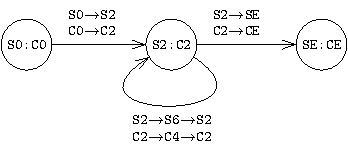
\includegraphics[scale=1.2]{chapters/figures/figStrlenArrProductCfg.pdf}}
\end{center}
\caption{\label{fig:StrlenArrProductCFG}Product-CFG for programs \cref{fig:llStrlenSpecIR,fig:llStrlenCArrIR}}
\end{subfigure}%
&
\begin{subfigure}[b]{0.50\textwidth}
\begin{center}
\begin{scriptsize}
\begin{tabular}{cl}
\toprule
{\bf PC-Pair} & \multicolumn{1}{c} {\bf Invariants} \\
\toprule
(\scpc{0}{0}) &
\Tstrut $\circled{P}\ \sv{s} \indEq{} \lifted{str}{\mem{}}{char[]}{\cv{s}}$ \\
\midrule
\multirow{2}{*}{(\scpc{2}{2})} &
\Tstrut $\circled{\tiny I1} \ \sv{s} \indEq{} \lifted{str}{\mem{}}{char[]}{\cv{s}}$ \\ &
\Tstrut $\circled{\tiny I2} \ \sv{len} = \cv{i}$ \\
\midrule
(\scpc{E}{E}) &
\Tstrut \Bstrut $\circled{E}\ \sv{ret} = \cv{ret}$ \\
\bottomrule
\end{tabular}
\end{scriptsize}
\end{center}
\caption{\label{fig:StrlenArrInvs}Invariants for product-CFG in \cref{fig:StrlenArrProductCFG}}
\end{subfigure}%
\\
\begin{subfigure}[b]{0.50\textwidth}
\begin{center}
{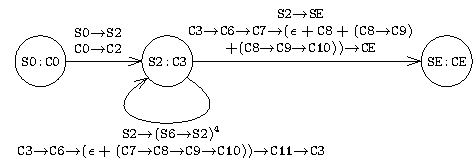
\includegraphics[scale=1.15]{chapters/figures/figStrlenClProductCfg.pdf}}
\end{center}
\caption{\label{fig:StrlenClProductCFG}Product-CFG for programs \cref{fig:llStrlenSpecIR,fig:llStrlenCClistIR}}
\end{subfigure}%
&
\begin{subfigure}[b]{0.50\textwidth}
\begin{center}
\begin{scriptsize}
\begin{tabular}{cl}
\toprule
{\bf PC-Pair} & \multicolumn{1}{c} {\bf Invariants} \\
\toprule
(\scpc{0}{0}) &
\Tstrut $\circled{P}\ \sv{s} \indEq{} \lifted{str}{\mem{}}{clnode}{\cv{cl},0}$ \\
\midrule
\multirow{2}{*}{(\scpc{2}{3})} &
\Tstrut $\circled{\tiny I1} \ \sv{s} \indEq{} \lifted{str}{\mem{}}{clnode}{\cv{cl},0}$ \\ &
\Tstrut $\circled{\tiny I2} \ \sv{len} = \cv{i}$ \\
\midrule
(\scpc{E}{E}) &
\Tstrut \Bstrut $\circled{E} \ \sv{ret} = \cv{ret}$ \\
\bottomrule
\end{tabular}
\end{scriptsize}
\end{center}
\caption{\label{fig:StrlenClInvs}Invariants for product-CFG in \cref{fig:StrlenClProductCFG}}
\end{subfigure}%
\end{tabular}
\caption{\label{fig:StrlenProductCFGsAndInvs}Product-CFGs and their node invariants representing bisimulation relations between the specification \cref{fig:llStrlenSpecIR}
and its two implementations in \cref{fig:llStrlenCArrIR,fig:llStrlenCClistIR} respectively.}
\end{figure}

\begin{center}
\begin{table}[H]
\begin{scriptsize}
\begin{tabular}{|l|l|}
\hline
\multicolumn{1}{|c|}{\Tstrut \Bstrut\footnotesize Lifting Constructor} & \multicolumn{1}{c|}{\Tstrut \Bstrut \footnotesize Definition} \\
\hline
\hline
\multicolumn{2}{|c|}{\Tstrut \Bstrut \inv{T1} {\tt Str = SInvalid | SNil | SCons(ch:i8, tail:Str)}} \\
\hline
$\mathrm{Cstr^{char[]}_m(p:i32)}$ & \makecell[l]{\Tstrut $\mathrm{\underline{if}\ (p==0_{i32})}$ $\mathrm{\underline{then}\ SInvalid}$ \\ \Tstrut $\mathrm{\underline{else\ if}\ (p[0_{i32}]^m_{i8}==0_{i8})\ \underline{then}\ SNil}$ \\ \Bstrut $\mathrm{\underline{else}\ SCons(p[0_{i32}]^m_{i8}, Cstr^{char[]}_m(p+1_{i32}))}$} \\
\hline
$\mathrm{Cstr^{lnode(char)}_m(p:i32)}$ & \makecell[l]{\Tstrut $\mathrm{\underline{if}\ (p==0_{i32})}$ $\mathrm{\underline{then}\ SInvalid}$ \\ \Tstrut $\mathrm{\underline{else\ if}\ (\structPointer{\tt p}{m}{\tt lnode}{val} == 0_{i8})\ \underline{then}\ SNil}$ \\ \Bstrut $\mathrm{\underline{else}\ SCons(\structPointer{\tt p}{m}{\tt lnode}{val}, Cstr^{lnode}_m(\structPointer{\tt p}{m}{\tt lnode}{next}))}$} \\
\hline
$\mathrm{Cstr^{clnode(char)}_m(p:i32,i:i2)}$ & \makecell[l]{\Tstrut $\mathrm{\underline{if}\ (p==0_{i32})}$ $\mathrm{\underline{then}\ SInvalid}$ \\ \Tstrut $\mathrm{\underline{else\ if}\ (\structPointer{\tt p}{m}{\tt clnode}{chunk} [i]^m_{i8} == 0_{i8})\ \underline{then}\ SNil}$ \\ \Bstrut $\mathrm{\underline{else}\ SCons(\structPointer{\tt p}{m}{\tt clnode}{chunk} [i]^m_{i8},}$ \\ \qquad \qquad \quad $\mathrm{Cstr^{clnode}_m((ite(i==3_{i2},\structPointer{\tt p}{m}{\tt clnode}{next} , p), i+1_{i2}))}$} \\
\hline
\end{tabular}
\end{scriptsize}
\caption{\label{tab:LiftingConsStr}Lifting constructors and their definitions for {\tt String} ADT.}
\vspace{-18px}
\end{table}
\end{center}


\subsubsection{List}
We wrote a \SpecL{} program specification that creates a list, a
program that traverses a list to compute the sum of its elements and a program
that computes the dot product of two lists. We use three different
data layouts for a list in C: array (\lift{list}{\mem{}}{u32[]}),
linked list (\lift{list}{\mem{}}{lnode(u32)}), and
a chunked linked list (\lift{list}{\mem{}}{clnode(u32)}).
The lifting constructors are shown in \cref{tab:LiftingConsList}.
Although similar to the String lifting constructors, these lifting
constructors differ widely in their data encoding. For example,
\lifted{list}{\mem{}}{u32[]}{p,i,n} represents a \type{List} value constructed
from a C array $p$ of size $n$ starting at the $i^{th}$ index. The list becomes empty
when we are at the end of the array. (\lift{list}{\mem{}}{lnode(u32)})
and (\lift{list}{\mem{}}{clnode(u32)}), on the other hand, encodes empty
lists (\cons{LNil}) using {\em null pointers}. These layouts are in contrast to the
\type{String} layouts, all of which uses a {\em null character} to
indicate the empty string.

\begin{table}[H]
\begin{center}
\caption{\label{tab:LiftingConsTree}Tree lifting constructors and their definitions.}
\begin{scriptsize}
\begin{tabular}{|l|l|}
\hline
\multicolumn{1}{|c|}{\Tstrut \Bstrut\footnotesize \bf Lifting Constructor} & \multicolumn{1}{c|}{\Tstrut \Bstrut \footnotesize \bf Definition} \\
\hline
\hline
\multicolumn{2}{|c|}{\Tstrut \Bstrut \inv{T3} {\tt Tree = TNil | TCons(i32, Tree, Tree)}} \\
\hline
\lifted{tree}{\mem{}}{u32[]}{p\ i\ n\ctype{i32}} & \makecell[l]{\Tstrut \sumIf{i \geq_u n} \  \sumThen{\cons{TNil}} \\
                                                        \Tstrut \Bstrut \sumElse{\cons{TCons}(\arrIndex{p}{i}{i32}{\mem{}}, \lifted{tree}{\mem{}}{u32[]}{p,2_\type{i32} \times i+1_\type{i32},n}, \lifted{tree}{\mem{}}{u32[]}{p,2_\type{i32} \times i+2_\type{i32},n})}} \\
\hline
\lifted{tree}{\mem{}}{tnode(u32)}{p\ctype{i32}} & \makecell[l]{\Tstrut \sumIf{p = 0_\type{i32}} \  \sumThen{\cons{TNil}} \\
                                                       \Tstrut \Bstrut \sumElse{\cons{TCons}(\structPointer{p\!}{\mem{}}{tnode}{\!\!val},\! \lifted{tree}{\mem{}}{tnode(u32)}{\structPointer{p\!}{\mem{}}{tnode}{\!\!left}},\! \lifted{tree}{\mem{}}{tnode(u32)}{\structPointer{p\!}{\mem{}}{tnode}{\!\!right}})}} \\
\hline
\end{tabular}
\end{scriptsize}
\end{center}
\end{table}

\subsubsection{Tree}
We wrote a \SpecL{} program that sums all the nodes in a tree
through an inorder traversal using recursion. We use two different data layouts for a tree: 
(1) a flat array where a
complete binary tree is laid out in breadth-first search order commonly used for heaps (\lift{tree}{\mem{}}{u32[]}),
and (2) a linked tree node with two pointers for the left and right children (\lift{tree}{\mem{}}{tnode(u32)}) (shown in \cref{tab:LiftingConsTree}).
Both \SpecL{} and C programs contain non-tail recursive procedure calls for left and right children.
\toolName{} is able to correlate these recursive calls using user-provided $Pre$ and $Post$.
At the entry of the recursive calls, \toolName{} is required to prove that $Pre$ holds for the arguments
and at the exit of the recursive calls, \toolName{} assumes $Post$ on the returned states.

\begin{table}[H]
\caption{\label{tab:LiftingConsMatrix}Matrix and auxiliary lifting constructors and their definitions.}
\vspace{-10px}
\begin{scriptsize}
\begin{center}
\begin{tabular}{|l|l|}
\hline
\multicolumn{1}{|c|}{\Tstrut \Bstrut\footnotesize Lifting Constructor} & \multicolumn{1}{c|}{\Tstrut \Bstrut \footnotesize Definition} \\
\hline
\hline
\multicolumn{2}{|c|}{\Tstrut \Bstrut \inv{T4} {\tt Matrix = MNil | MCons(List, Matrix)}} \\
\hline
$\mathrm{Cmat^{u32[][]}_m(p\ i\ u\ v:i32)}$ & \makecell[l]{\Tstrut $\mathrm{\underline{if}\ (i \geq_{u} u)}$ $\mathrm{\underline{then}\ MNil}$ \\ \Bstrut $\mathrm{\underline{else}\ MCons(Clist^{u32[]}_m(p[i]^m_{i32},0_{i32},v), Cmat^{u32[][]}_m(p,i+1_{i32},u,v))}$} \\
\hline
\hline
$\mathrm{Clist^{u32[r]}_m(p\ i\ j\ u\ v:i32)}$ & \makecell[l]{\Tstrut $\mathrm{\underline{if}\ (j\geq_{u}v)}$ $\mathrm{\underline{then}\ LNil}$ \\ \Bstrut $\mathrm{\underline{else}\ LCons(p[i*v+j]^m_{i32}, Clist^{u32[r]}_m(p,i,j+1_{i32},u,v))}$} \\
\hline
$\mathrm{Cmat^{u32[r]}_m(p\ i\ u\ v:i32)}$ & \makecell[l]{\Tstrut $\mathrm{\underline{if}\ (i \geq_{u} u)}$ $\mathrm{\underline{then}\ MNil}$ \\ \Bstrut $\mathrm{\underline{else}\ MCons(Clist^{u32[r]}_m(p,i,0_{i32},u,v), Cmat^{u32[r]}_m(p,i+1_{i32},u,v))}$} \\
\hline
\hline
$\mathrm{Clist^{u32[c]}_m(p\ i\ j\ u\ v:i32)}$ & \makecell[l]{\Tstrut $\mathrm{\underline{if}\ (j\geq_{u}v)}$ $\mathrm{\underline{then}\ LNil}$ \\ \Bstrut $\mathrm{\underline{else}\ LCons(p[i+j*u]^m_{i32}, Clist^{u32[c]}_m(p,i,j+1_{i32},u,v))}$} \\
\hline
$\mathrm{Cmat^{u32[c]}_m(p\ i\ u\ v:i32)}$ & \makecell[l]{\Tstrut $\mathrm{\underline{if}\ (i \geq_{u} u)}$ $\mathrm{\underline{then}\ MNil}$ \\ \Bstrut $\mathrm{\underline{else}\ MCons(Clist^{u32[c]}_m(p,i,0_{i32},u,v), Cmat^{u32[c]}_m(p,i+1_{i32},u,v))}$} \\
\hline
\hline
$\mathrm{Cmat^{lnode(u32[])}_m(p\ v:i32)}$ & \makecell[l]{\Tstrut $\mathrm{\underline{if}\ (p==0_{i32})}$ $\mathrm{\underline{then}\ MNil}$ \\ \Bstrut $\mathrm{\underline{else}\ MCons(Clist^{u32[]}_m(\structPointer{\tt p}{m}{\tt lnode}{val},0_{i32},v),}$ \\ \qquad\qquad\ \ \ \  $\mathrm{Cmat^{lnode(u32[])}_m(\structPointer{\tt p}{m}{\tt lnode}{next},v))}$} \\
\hline
$\mathrm{Cmat^{lnode(u32)[]}_m(p\ i\ u:i32)}$ & \makecell[l]{\Tstrut $\mathrm{\underline{if}\ (i \geq u)}$ $\mathrm{\underline{then}\ MNil}$ \\ \Bstrut $\mathrm{\underline{else}\ MCons(Clist^{lnode(u32)}_m(p[i]^m_{i32}),}$ \\ \qquad\qquad\ \ \ \  $\mathrm{Cmat^{lnode(u32)[]}_m(p,i+1_{i32},u))}$} \\
\hline
$\mathrm{Cmat^{clnode(u32)[]}_m(p\ i\ u:i32)}$ & \makecell[l]{\Tstrut $\mathrm{\underline{if}\ (i \geq u)}$ $\mathrm{\underline{then}\ MNil}$ \\ \Bstrut $\mathrm{\underline{else}\ MCons(Clist^{clnode(u32)}_m(p[i]^m_{i32},0_{i2}),}$ \\ \qquad\qquad\ \ \ \  $\mathrm{Cmat^{clnode(u32)[]}_m(p,i+1_{i32},u))}$} \\
\hline
\end{tabular}
\end{center}
\end{scriptsize}
\end{table}


\subsubsection{Matrix}
We wrote a
\SpecL{} program to count the frequency of a value appearing in a 2D matrix.
A matrix is represented as an ADT that resembles a \type{List} of \type{List}s (\inv{\small T4} in \cref{tab:LiftingConsMatrix}).
The C implementations for a \type{Matrix} object include
(a) a two-dimensional array (\lift{mat}{\mem{}}{u32[][]}), (b) a flattened row-major array (\lift{mat}{\mem{}}{u32[r]}),
(c) a flattened column-major array (\lift{mat}{\mem{}}{u32[c]}), (d) a linked list of 1D arrays (\lift{mat}{\mem{}}{lnode(u32[])}),
(e) a 1D array of linked lists (\lift{mat}{\mem{}}{lnode(u32)[]}) and (f) a 1D array of chunked linked list (\lift{mat}{\mem{}}{clnode(u32)[]})
data layouts. Note that both \type{T[r]} and \type{T[c]} represent a 1D array of type {\tt T}. The {\em r} and {\em c} simply
emphasizes that these arrays are used to represent matrices in row-major and column-major encodings respectively.
We also introduce two auxiliary lifting constructors, \lift{list}{\mem{}}{u32[r]} and \lift{list}{\mem{}}{u32[c]}
for lifting each row of matrices lifted using the corresponding \lift{mat}{\mem{}}{u32[r]} and \lift{mat}{\mem{}}{u32[c]} \type{Matrix} lifting
constructors. These constructors are listed in \cref{tab:LiftingConsMatrix}.

\begin{figure}[H]
\begin{scriptsize}
\begin{tabular}{lllclllc}
\toprule
{\bf Data Layout} & {\bf Variant} & {\bf Time(s)} & {\bf ${\tt \bf ( d_u, d_o )}$} & {\bf Data Layout} & {\bf Variant} & {\bf Time(s)} & {\bf ${\tt \bf ( d_u, d_o )}$} \\
\midrule
\multicolumn{4}{c}{\bf list} &                                              \multicolumn{4}{c}{\bf tree} \\
u32[] & sum naive & 16 & (1,2) &                                           u32[] & sum & 264 & (1,2) \\
      & sum opt & 49 & (4,5) &                                             tnode(u32) & sum & 204 & (1,2) \\
lnode(u32) & sum naive & 8 & (1,2) &                                      \multicolumn{4}{c}{\bf matfreq} \\             
           & sum opt & 54 & (4,5) &                                       char[][] & naive & 974 & (1,3) \\                                      
           & create & 426 & (1,1) &                                                & opt & 1.8k & (4,8) \\                                       
clnode(u32) & sum opt & 39 & (4,5) &                                      char[r] & naive & 958 & (1,3) \\                                       
\multicolumn{4}{c}{\bf strlen}   &                                            & opt & 1.9k & (4,8) \\                                        
char[] & dietlibc$\mathrm{_{small}}$ & 9 & (1,2) &                             char[c] & naive & 984 & (1,3) \\                                       
       & dietlibc$\mathrm{_{fast}}$ & 44 & (3,2) &                                     & opt & 1.9k & (4,6) \\
       & glibc & 52 & (3,2) &                                                  lnode(char[]) & naive & 753 & (1,3) \\
       & klibc & 9 & (1,2) &                                                         & opt & 1.7k & (4,6) \\ 
       & musl & 49 & (3,2) &                                                   lnode(char)[] & naive & 1.5k & (1,2) \\
       & netbsd & 9 & (1,2) &                                                                & opt & 2.3k & (4,6) \\
       & newlib & 50 & (3,2) &                                              clnode(char)[] & opt & 1.8k & (4,6) \\
       & openbsd & 8 & (1,2) &                                                \multicolumn{4}{c}{\bf strpbrk} \\ 
       & uClibc & 8 & (1,2) &                                                 char[], char[] & dietlibc & 398 & (1,2) \\
lnode(char) & naive & 13 & (1,2) &                                                          & opt      & 494 & (4,2) \\
            & opt & 49 & (3,5) &                                              char[], lnode(char) & naive & 392 & (1,2) \\
clnode(char) & opt & 45 & (3,5) &                                                                & opt & 540 & (4,2) \\ 
 \multicolumn{4}{c}{\bf strchr} &                                                 char[], clnode(char) & opt & 523 & (4,2) \\
char[] & dietlibc$\mathrm{_{small}}$ & 16 & (1,1) &                           lnode(char), char[] & naive & 497 & (1,2) \\
       & dietlibc$\mathrm{_{fast}}$ & 89 & (4,1) &                                               & opt & 602 & (4,2) \\ 
       & glibc & 127 & (4,1) &                                                lnode(char), lnode(char) & naive & 345 & (1,2) \\
       & klibc & 23 & (1,1) &                                                                           & opt & 503 & (4,2) \\
       & newlib$\mathrm{_{small}}$ & 15 & (1,1) &                         lnode(char), clnode(char) & opt & 572 & (4,2) \\
       & openbsd & 24 & (1,1) &                                             \multicolumn{4}{c}{\bf strcspn} \\
       & uClibc & 22 & (1,1) &                                              char[], char[] & dietlibc & 462 & (1,2) \\ 
lnode(char) & naive & 19 & (1,1) &                                                        & opt      & 538 & (4,2) \\ 
            & opt & 146 & (4,1) &                                           char[], lnode(char) & naive & 395 & (1,2) \\
\multicolumn{4}{c}{\bf strcmp}   &                                     & opt & 521 & (4,2) \\
char[], char[] & dietlibc$\mathrm{_{small}}$ & 39 & (1,1) &                 char[], clnode(char) & opt & 527 & (4,2) \\
       & freebsd & 39 & (1,1) &                                             lnode(char), char[] & naive & 601 & (1,2) \\
       & glibc & 41 & (1,1) &                                                                  & opt & 660 & (4,2) \\ 
       & klibc & 41 & (1,1) &                                               lnode(char), lnode(char) & naive & 349 & (1,2) \\
       & musl & 41 & (1,1) &                                                                        & opt & 502 & (4,2) \\
       & netbsd & 39 & (1,1) &                                              lnode(char), clnode(char) & opt & 595 & (4,2) \\
       & newlib$\mathrm{_{small}}$ & 42 & (1,1) &                              \multicolumn{4}{c}{\bf strspn} \\
       & newlib$\mathrm{_{fast}}$ & 405 & (4,1) &                              char[], char[] & dietlibc & 277 & (1,2)                   \\
       & openbsd & 40 & (1,1) &                                                              & opt      & 388 & (4,2)                    \\
       & uClibc & 38 & (1,1) &                                                 char[], lnode(char) & naive & 405 & (1,2)                 \\
lnode(char), lnode(char) & naive & 47 & (1,1) &                                                   & opt & 682 & (4,2)                    \\ 
            & opt & 293 & (4,1) &                                              char[], clnode(char) & opt & 535 & (4,2)                  \\
clnode(char), clnode(char) & opt & 254 & (4,1) &                               lnode(char), char[] & naive & 409 & (1,2)           \\
\multicolumn{4}{c}{\bf vecdot} &                                                          & opt & 553 & (4,2)              \\
u32[] & naive & 65 & (1,2) &                                                  lnode(char), lnode(char) & naive & 357 & (1,2)        \\
      & opt & 176 & (4,5)   &                                                                          & opt & 514 & (4,2)        \\
lnode(u32) & naive & 37 & (1,2) &                                              lnode(char), clnode(char) & opt & 616 & (4,2)         \\
           & opt & 120 & (4,5)   &                                               & & & \\
clnode(u32) & opt & 118 & (4,5)   &                                               & & & \\
\bottomrule
\end{tabular}
\end{scriptsize}
\vspace{-5px}
\caption{\label{tab:results}Equivalence checking times and minimum under- and over-approximation depth values at which equivalence checks succeeded.}
\vspace{-5px}
\end{figure}

\subsection{Results}
\label{sec:results}
\Cref{tab:results} lists the various C implementations and the time it took
to compute equivalence with their specifications. For functions that
take two or more data structures as arguments, we show
results for different combinations of data layouts for each argument.
We also show the minimum under-approximation ($d_u$) and over-approximation ($d_o$) depths
at which the equivalence proof completed (keeping all other parameters to their
default values).

During the verification of {\tt strchr} and {\tt strpbrk} implementations,
we identified an interesting subtlety. Since {\tt strchr} and {\tt strpbrk}
return null pointers to signify absence of the required character(s) in the input string,
we additionally need to model the UB assumption that the zero
address does not belong to the null character terminated array representing the string.
We use an explicit constructor \cons{SInvalid} to expose this well-formedness property in a \SpecL{} \type{String}.
Furthermore, we relate \cons{SInvalid} to the condition of C character pointer being null using the
lifting constructors \lifted{str}{\mem{}}{T}{p\ctype{i32},\dots} (as defined in \cref{tab:LiftingConsList}).
These lifting constructors are used as part of $Pre$ to equate $S$ and $C$ input strings.
Finally in $S$, we model the absence of \cons{SInvalid} in the input string as a UB assumption using
the {\tt assuming-do} statement introduced in \cref{sec:speclang}.
Due to the \sdef{} assumption, this constraints the inputs to $S$ as well as $C$ to well-formed strings only.
This is an example where \sdef{} and $Pre$ can be used to model wellformedness of values in $C$.

TODO: add strlen spec atleast, show the strchr also!! maybe some matrix data layouts (only layouts)

\subsection{Limitations}
\label{sec:limitations}
Our proof discharge algorithm is not without limitations.
For a \recursiveRelation{} relating values of a non-linear ADT such as \type{Tree}, a $d$-depth
approximation results in $\sim 2^d$ smaller equalities. This is a major cause of inefficiency due to
generation of large queries which slows down SMT solvers and counterexample-guided algorithms for large values of $d$.

\toolName{} is only interested in finding a bisimulation relation and hence
equivalence of non-bisimilar programs is beyond our scope.
\toolName{} currently only supports bitvector affine and inequality relations
along with \recursiveRelations{} provided as part of $Pre$ and $Post$.
Consequently, non-linear bitvector invariants (e.g. polynomial invariants)
as well as custom \recursiveRelations{} are not supported.
While our correlation and invariant inference algorithms based on the Counter tool \cite{oopsla20}
are designed for translation validation between (C-like) unoptimized IR and assembly, we found them
to be surprisingly good for \SpecL{} to (C-like) IR as well. Rather unsurprisingly, \toolName{}
suffers from the same limitations of these algorithms. For example, \toolName{} supports path
specializations from \SpecL{} to C, it does not search for path merging correlations.
\section{Conclusion}
\label{sec:conclusion}
As introduced in \cref{sec:syn-intro}, most of the current solutions
to the problem of equivalence checking between a functional specification
and a C program relies heavily on manually provided correlation, inductive
invariants as well as proof assistants for discharging said obligations.
While the size of programs considered in our work is quite small,
we hope the ideas in \toolName{} will help
automate the proofs for such systems to some degree.

Prior work on push-button verification of specific
systems \cite{fscq,hyperkernel,serval,verifiedBPF}
involves a combination of careful system design and
automatic verification tools like SMT solvers.
Constrained Horn Clause (CHC) Solvers \cite{CHCeq}
encode verification conditions of programs containing loops and recursion,
and raise the level of abstraction for automatic proofs.
Comparatively, \toolName{} further raises the level
of abstraction for automatic verification from
SMT queries and CHC queries to automatic discharge of
proof obligations involving \recursiveRelations{}.

A key idea in \toolName{} is the conversion of proof
obligations involving \recursiveRelations{} to
bisimulation checks. Thus, \toolName{} performs {\em nested}
bisimulation checks as part of a `higher-level'
bisimulation search. This approach of
identifying \recursiveRelations{} as invariants and using
bisimulation to discharge the associated
proof obligations may have applications
beyond equivalence checking.


\pagestyle{fancy}
\cleardoublepage
%------------------------------------------------------------------------- 
\addtocontents{toc}{\vspace{1em}} % Add a gap in the Contents, for aesthetics

\cleardoublepage
\addcontentsline{toc}{chapter}{Bibliography}
\bibliographystyle{plain} 
\bibliography{main}

%\cleardoublepage
\pagestyle{plain}
\doublespacing
\cleardoublepage

\addcontentsline{toc}{chapter}{Biography}
\chapter*{Biography}

Indrajit Banerjee is a MS(by research) student of Computer Science and Engineering department at IIT Delhi.
He is a B.Tech. gold medalist in Electronics and Communication Engineering from Institute of Engineering \&
Management (IEM), Kolkata.
During his undergraduate course, he was a summer research intern at
Center for Integrative Biology and Systems medicinE (IBSE) in IIT Madras.
Due to an afinity towards research exposed during this time, he chose to persue
a research-oriented postgraduation program right after his B.Tech.
His research interests include: compilers, formal verification and linear algebra.


\cleardoublepage
\pagestyle{plain}

\end{document}	
